\documentclass[11pt,twoside]{scrreprt}
\usepackage[utf8]{inputenc} 	%package pour le français sous ubuntu : à vous d'adapter
\usepackage[french]{babel}	%pour le français
\usepackage[T1]{fontenc}	%pour les polices
\usepackage{amsmath}		%pour des maths
\usepackage{amsfonts}		%pour des maths
\usepackage{amssymb}		%pour des maths
\usepackage{graphicx}		%pour les inclusions de graphiques
\usepackage{times}		%choix personnel de police : Times New Roman 
\usepackage{lscape}		%si vous voulez des images en paysage
\usepackage{hyperref}		%pour les liens croisés à travers le fichier .pdf
\usepackage{fancyhdr}		%pour les marges
\usepackage{float, caption}	%pour le positionnement et légende des images
\usepackage{color}		%pour la couleur dans le code
\usepackage{listings}		%pour mettre du code, plutôt en Annexe
\usepackage{lastpage}		%pour les références aux pages
\usepackage{epic,eepic}		%pour le positionnement de l'image de garde
\usepackage{wrapfig}		%pour les images sur le coté dans le texte
\usepackage{calc,ifthen,xspace}	%pour redéfinir les espaces et distances
\usepackage{scrlfile}
\usepackage{soul} %surlignance
\PreventPackageFromLoading{fp}
\usepackage[final]{pdfpages} % Pour inclure un pdf
\usepackage[titletoc]{appendix} % Pour les annexes
\usepackage{glossaries} % Pour le lexique
\usepackage{tabularx}
\usepackage{diagbox}
\ResetPreventPackageFromLoading
\usepackage{array}
\pagestyle{fancy}
\AddThinSpaceBeforeFootnotes 
\FrenchFootnotes 
\makeglossaries
\usepackage{lmodern}
\usepackage{textcomp}
\usepackage{xspace}
\usepackage{listingsutf8}
\usepackage{xcolor}
\usepackage{afterpage}
\usepackage{url}
\usepackage[top=2.1cm,bottom=2.3cm,left=2cm,right=2cm]{geometry}
\usepackage{multirow}
\usepackage{verbatim}

% Pour sommaire cliquable 

\hypersetup{
dvips,
backref=true, %permet d'ajouter des liens dans...
pagebackref=true,%...les bibliographies
hyperindex=true, %ajoute des liens dans les index.
colorlinks=false, %colorise les liens
breaklinks=true, %permet le retour à la ligne dans les liens trop longs
urlcolor= blue, %couleur des hyperliens
linkcolor= blue, %couleur des liens internes
bookmarks=blue, %créé des signets pour Acrobat
bookmarksopen=true} 

\definecolor{hellgelb}{rgb}{1,1,0.8} % couleur pour le code
\definecolor{colKeys}{rgb}{0,0,1}
\definecolor{colIdentifier}{rgb}{0,0,0}
\definecolor{colComments}{rgb}{0,0.5,0}
\definecolor{colString}{rgb}{0.62,0.12,0.94}
\definecolor{INSA_GM}{cmyk}{0.6,0,0,0} % et la page de garde
\definecolor{INSA_GRIS}{cmyk}{0.7,0.6,0.5,0.3}
\definecolor{INSA_BLEU}{cmyk}{1,0.9,0.1,0}
\definecolor{mygreen}{rgb}{0,0.6,0}
\definecolor{mygray}{rgb}{0.5,0.5,0.5}
\definecolor{mymauve}{rgb}{0.58,0,0.82}
\definecolor{mygrayblack}{rgb}{0.32,0.32,0.32}
\colorlet{punct}{red!60!black}
\definecolor{background}{HTML}{EEEEEE}
\definecolor{delim}{RGB}{20,105,176}
\colorlet{numb}{magenta!60!black}

\usepackage{templateINSA}
\initINSA

% Titre centre
\renewcommand\infoBig{Leriche Florian}
\renewcommand\infoSmall{Rapport de stage ingénieur}

% Titre bas 
\title{Transformation digitale des banques}
\renewcommand\soustitre{Sopra Steria Group}

% Auteurs
\author{ 
	\textbf{Étudiant :} \bsc{Leriche} Florian\\
	\textbf{Maîtres de stage :} \bsc{Berthaud} Laurent, \bsc{Sacenda} Cyril \\
	\textbf{Entreprise :} Sopra Steria\\
	\textbf{Clients :} BP1818, Neuflize OBC\\
	\textbf{Date :} 13/02/2017 - 11/08/2017\\
	\textbf{Lieu :} Paris, France\\
}

\begin{document}
\thispagestyle{empty}
% titleINSA : Page de garde 
% #1 : descendre le titre du milieu (en mm)
% #2 : lien de l'image de fond
% #3 : décalage sur X de l'image de fond (en mm)
% #4 : décalage sur Y de l'image de fond (en mm)
% #5 : largeur de l'image de fond de #5 (en mm)
% #6 : Crédit de l'image de fond
\titleINSA{15}{images/fond.jpg}{-20}{60}{250}{Image : \href{http://img.decision-achats.fr/Img/BREVE/2016/1/300834/Digitalisation-opportunite-achats-porteurs-innovation--F.jpg}{\color{white}{http://img.decision-achats.fr/}}}

\thispagestyle{empty}

%-----------------------------------------------------------------------------------------------------------------
%-----------------------------------------------------------------------------------------------------------------
	\tableofcontents
	\addtocontents{toc}{\protect\thispagestyle{empty}}
	\thispagestyle{empty}
%-----------------------------------------------------------------------------------------------------------------
%-----------------------------------------------------------------------------------------------------------------

\newpage

\chapter*{Remerciements}
	\addcontentsline{toc}{chapter}{Remerciements}
	\setcounter{page}{1}
	\setcounter{tocdepth}{1}
\hl{TODO}

%-----------------------------------------------------------------------------------------------------------------
%-----------------------------------------------------------------------------------------------------------------
	\chapter*{Introduction}				% garde la même mise en page qu'un chapitre mais ne le numérote pas
	\addcontentsline{toc}{chapter}{Introduction}	% permet de l'avoir dans le sommaire

\paragraph{}
Le présent rapport détail le travail qui s’inscrit dans le cadre de la réalisation d’un stage ingénieur effectué par les élèves ingénieurs de l’Institut National des Sciences Appliquées de Rouen. Celui-ci s’est déroulé via la participation à deux missions distinctes pour le compte de la société de services \textit{Sopra Steria} du 13 février au 12 juillet 2017; suite à une convention tripartite signée entre le département Architecture des Systèmes d’Information de L’INSA, l’entreprise d’accueil et moi-même. Pendant ce stage, j’ai eu l’occasion de participer à plusieurs projets qui m’ont permis d’appréhender le métier d’ingénieur en informatique, d’acquérir de l’expérience ainsi que de m’épanouir aussi bien dans le plan personnel que professionnel.

\paragraph{}
La première mission à laquelle j'ai pris part s'est déroulée du 13 février 2017 jusqu'à la fin de mon stage, pour le compte du client \textit{Neuflize OBC}. La seconde mission a débuté le 29 mars 2017 pour la banque privée \textit{BP1818} et s'est déroulée en parallèle de la première jusqu'à la fin du stage. La répartition du temps de travail était la suivante :
\begin{itemize}
	\item Lundi, mardi et vendredi chez le client \textit{BP1818}
	\item Mercredi et jeudi chez le client \textit{Neuflize OBC}
\end{itemize}

\paragraph{}
Sopra Steria est une entreprise de services du numérique et l'un des leader européens dans la transformation numérique. Ainsi, l'objectif premier de mon stage a été d'accompagner certains des clients banques privées de Sopra Steria dans leur transformation digital en travaillant à la fois sur la réalisation et l'industrialisation d'une application mobile à destination des clients de la banque Neuflize ainsi que sur la mise en place d'une application web à destination des banquiers travaillant chez BP1818.

\paragraph{}
Dans un premier temps, je présenterai l'entreprise d'accueil et les client pour lesquels j'ai travaillé, leurs domaines d’activités, leurs origines, leurs personnel ainsi que leurs locaux.
Dans un second temps, je détaillerai de manière précise les sujets des missions qui m’ont été confiées au sein des équipes.
Enfin, je décrirai en profondeur le déroulement de mon stage ainsi que les différents travaux que j’ai accompli et les conditions dans lesquelles je les ai réalisé. 

\paragraph{}
Pour des raisons de clarté et de cohérence, ce rapport présentera deux parties distinctes concernant le déroulement du stage, chacune ayant pour objectif de décrire le travail réalisé chez les clients cités plus haut et suivant le même schéma.
%-----------------------------------------------------------------------------------------------------------------
%-----------------------------------------------------------------------------------------------------------------

%-----------------------------------------------------------------------------------------------------------------
%-----------------------------------------------------------------------------------------------------------------	
\chapter{Présentation de l'entreprise}

	\section{Historique}
	\paragraph{}
\textit{Sopra Steria} est une entreprise de services du numérique (ESN) résultant de la fusion, en janvier 2015, de deux des plus anciennes sociétés de services en ingénierie informatique françaises, \textit{Sopra} et \textit{Steria}.

\subsection{1968 - 1985 : Les débuts}

\paragraph{}
Création des sociétés Sopra et Steria respectivement en 1968 et 1969, période marquée par la naissance de l'industrie des services informatiques.\\

La \textbf{SO}ciété de \textbf{PR}ogrammation et d'\textbf{A}nalyses (Sopra), fondée par Pierre Pasquier et François Odin, est avant tout une entreprise de services de conseils technologiques spécialisée dans l'édition de logiciel. Elle signera, quelques années plus tard, son premier grand contrat d'infogérance bancaire qui marquera son initiation au savoir-faire relatif à la banque. Cela aboutira à la création de la première plateforme bancaire de Sopra qui proposera par la suite des logiciels à destination des banques. Par la suite, l'édition de solutions bancaires deviendra son activité phare avec la mise en production de sa première application concernant les crédits.\\

La \textbf{S}ocié\textbf{T}é d'\textbf{E}tude et de \textbf{R}éalisation en \textbf{I}nformatique et \textbf{A}utomatisme (Steria) contrôlée par Jean Carteron est aussi une société de services informatiques. L'informatisation de l'Agence France Presse est désignée comme étant l'une des première prouesse de la société qui participera par la suite au développement du minitel en travaillant sur la conception de son architecture.

\subsection{1985 - 2000 : Croissance et entrée en bourse}

\paragraph{}
Sopra repense sa structure industrielle en décidant de se recentrer sur des activités précises telles que l'intégration de systèmes et l'édition de logiciels et décroche son premier grand projet national avec le ministère de l'intérieur. Elle est introduite en Bourse en 1990 et multiplie les contrats ainsi que les acquisitions avec, par exemple, le rachat de \textit{SG2 ingénierie} marquant une forte croissance. Elle profitera de ses performances pour étendre son expertise à l'échelle internationale en s'implentant dans différents pays tels que le Royaume-Uni ou encore l'Allemagne.\\

De même, Steria étend son influence en dehors de la France, jusqu'en Arabie Saoudite où elle réalisera le système informatique de la banque centrale saoudienne. Elle intégrera le marché des transports à son domaine d'expertise, notamment grâce au projet d'automatisation du RER A en France, à Paris. Ses futures acquisitions lui permettront une entrée en Bourse en 1999.\\

\subsection{2000 - 2014 : Transformation numérique}

\paragraph{}
L'essor des technologies du numériques, à savoir l'informatique et internet, provoque une mutation des marchés qui a pour conséquence d'apporter de nombreux clients potentiels à la recherche de partenaires pouvant les accompagner dans leur transformation numérique. Les deux sociétés répondront à cette problématique et développeront leurs activités de conseil. Sopra crééra sa filiale \textit{Axway} regroupant ses activités dans le domaine du progiciel et qui entrera aussi en Bourse de manière autonome en 2011. Toujours fortement impliquée dans le domaine bancaire, elle décidera de créer sa filiale \textit{Sopra Banking Software} en 2012 et réalisera de nombreux projets avec les grands noms du secteur bancaire français (Crédit agricole, Société général, BNP, etc...)\\

Steria, de son côté, se retrouvera dans un contexte économique difficile et vera le prix de son action chuter. Elle continuera malgré tout de multiplier les acquisitions (\textit{Bull} en Europe, \textit{Mummert Consulting} en Allemagne ou encore \textit{Xansa} au Royaume-Uni). Elle remportera plusieurs des plus gros contrats (notamment SSCL pour la gestion du back office de plusieurs ministères de l'administration britannique) de son histoire avec le gouvernement britannique.

\subsection{2014 - 2016 : Fusion absorption}

\paragraph{}

En 2014, Sopra, forte d'une grande croissance, prend la décision d'absorber Steria en devenant actionnaire majoritaire à plus de 90\%. Il s'agit là d'une excellente opportunité misant sur la complémentarité des deux géants de l'informatique aussi bien sur le plan métier que sur le plan géographique. \\

En effet, comme nous l'avons dit plus haut, Steria est très présente au Royaume-Uni contrairement à Sopra. De plus, Sopra se vera ainsi faire l'acquisition de nombreux centres de compétences qui viendront renforcer son écrasante influence à travers l'europe. Les deux entreprises partagent beaucoup de points communs tels que la taille, les domaines d'activités ou encore les objectifs, ce qui constitue un atout majeur concernant leur fusion et leur projets d'avenir. \\

La fusion des deux groupes donne donc naissance à Sopra Steria, une entreprise possédant un poids écrasant, un capital titanesque permettant de gagner la confiance de nombreux clients ainsi qu'une très grande expertise lui permettant de mener à bien beaucoup de projets emblématiques tels que : \\

\begin{figure}[h]
	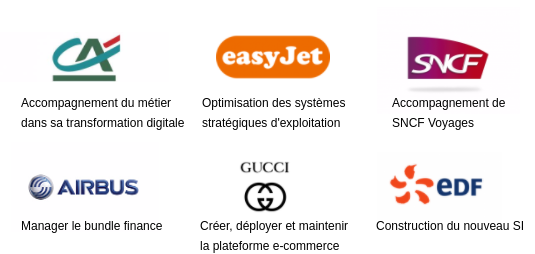
\includegraphics[scale=0.8]{images/projetsEmblematiques.png}
	\centering
	\caption{Projets emblématiques}
	\label{projetsEmblematiques}
\end{figure}
		

\section{Domaine d'activités}
	\begin{figure}[h]
	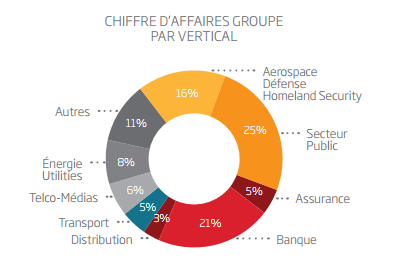
\includegraphics[scale=1]{images/sopraSteriaActivites.png}
	\centering
	\caption{Répartition des activités}
	\label{sopraSteriaActivites}
\end{figure}
		

\section{Quelques chiffres}
	\begin{figure}[h]
	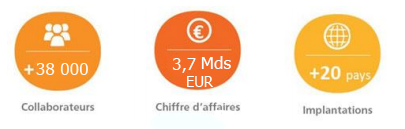
\includegraphics[scale=1]{images/sopraSteriaChiffres.png}
	\centering
	\caption{Quelques chiffres}
	\label{sopraSteriaChiffres}
\end{figure}

\begin{figure}[h]
	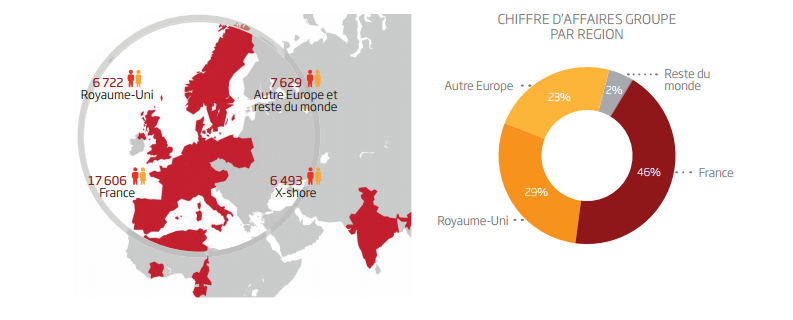
\includegraphics[scale=0.9]{images/sopraSteriaMonde.png}
	\centering
	\caption{Répartition internationale}
	\label{sopraSteriaMonde}
\end{figure}
		
		
	
\section{Organisation}
	\paragraph{}
L'organisation du groupe Sopra Steria est articulée autour de différentes structures opérationnelles et fonctionnelles donc une structure permanente globale décrite sur la figure \ref{sopraSteriaOrganisation}.

\begin{figure}[h]
	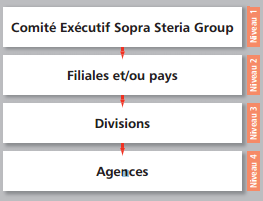
\includegraphics[scale=0.8]{images/sopraSteriaOrganisation.png}
	\centering
	\caption{Organisation du groupe}
	\label{sopraSteriaOrganisation}
\end{figure}
		
\subsubsection{Comité exécutif}
\paragraph{}
Le comité exécutif est composé du directeur général ainsi que de l'ensemble des directeurs adjoints et est en charge de piloter les projets et affaires les plus importantes du groupe. Il gère aussi l'organisation de la société dans son ensemble.

\subsubsection{Filiales et/ou pays}
\paragraph{}
Cette section désigne l'ensemble des grandes entités qui représente soit une partie métier dont nous avons parlé plus haut (conseil, BPS, etc...) soit une zone géographique pouvant faire référence à un pays complet. Ces parties sont alors ensuite découpées en un ensemble de divisions.

\subsubsection{Divisions}
\paragraph{}
Les divisions sont créées en fonction de la géographie ainsi que du secteur économique concerné (bancaire, transport, tertiaire etc...).

\subsubsection{Agences}
\paragraph{}
Enfin, les divisions sont constituées d'agences qui agissent de manière autonome concernant la gestion de leur budget, des ressources humaines ou encore du pilotage des projets.

\paragraph{}
Dans mon cas, j'ai été assigné à l'agence 512 de la division Banque et Finance de Sopra Steria France (TODO: à confirmer). Ainsi, les missions sur lesquelles j'ai été assigné était cohérentes avec la division dont je dépendais et concernaient toutes deux des clients banque privée dont je vais parler plus en détails dans la partie suivante.
		
\section{Partenaires et clients}
	\subsection{Neuflize OBC}

\begin{figure}[h]
	
\includegraphics[scale=0.3]{images/neuflizeOBCLogo.png}
	\centering
%	\caption{Logo Neuflize OBC}
	\label{neuflizeOBCLogo}
\end{figure}

\subsection{BP1818}

\begin{figure}[h]
	
\includegraphics[scale=0.3]{images/bp1818Logo.png}
	\centering
%	\caption{Logo BP1818}
	\label{bp1818Logo}
\end{figure}
		
		
%-----------------------------------------------------------------------------------------------------------------
%-----------------------------------------------------------------------------------------------------------------

%-----------------------------------------------------------------------------------------------------------------
%-----------------------------------------------------------------------------------------------------------------

\chapter{Présentation des sujets}
	
		Le secteur bancaire est actuellement en effervescence, impacté par la venue de nombreux nouveaux acteurs qui viennent bouleverser les règles établies. En effet, le progrès dans le domaine de l'informatique a permis de fournir des services inédits pouvant répondre aux attentes de la nouvelle génération de clients marquée par l'essor des technologies du numérique. Ainsi, de nouveaux acteurs sont apparus : les banques en ligne, c'est-à-dire des banques uniquement disponibles sur internet. Ces dernières ne possèdent pas de locaux physiques et n'ont que très peu de personnel. Néanmoins, elles sont capables de permettre à leurs clients de suivre l'état de leur compte bancaire ou patrimoine financier en temps réel. Il est possible de commander une carte bleue, un chéquier ou encore d'obtenir un rib sans avoir à se déplacer et bien d'autres services sont disponibles selon les banques et cela gratuitement. Les coûts de gestion des ressources humaines, d'organisation ou encore de matériels sont grandement réduits ce qui permet à ces nouvelles banques de pouvoir défier les grands groupes présents à l'échelle internationale. Ces derniers ont donc la nécessité de réagir afin de rester compétitifs sur ce marché en pleine évolution. \\

	On parle ainsi de transformation digitale des banques pour désigner la transition marquée par le processus de dématérialisation de l'économie en faisant appel aux technologies modernes. Neuflize OBC, comme nous l'avons vu dans la partie précédente, est une banque privée. Cette dernière est actuellement en cours de transformation afin de pouvoir répondre aux besoins de ses clients. Un \href{https://www.neuflizeobc.net/portail/portail.jsp}{site web} permettant de proposer les services dits "banque au quotidien" qui regroupe les fonctionnalités classiques à savoir consultation de comptes, impression de rib ou encore réalisation d'une transaction bancaire existe depuis plusieurs années. Cependant, les exigences sont toujours plus élevées, la génération actuelle étant toujours connectée via l'utilisation d'un smartphone, Neuflize a le besoin de produire une application mobile dans le but de permettre à ses clients de pouvoir accéder à leurs informations n'importe où et n'importe quand. \\

	L'équipe de développement constituée par Sopra Steria était en charge de la réalisation de la partie \textit{backend} de l'application, la partie \textit{frontend} ayant été déléguée à l'équipe qui a conçu le site web. Neuflize a décidé d'exposer des API dans le but de permettre la réalisation d'échanges au sein de son SI et vers l'extérieur. Ainsi, une architecture multicouches a été mise en place avec notamment :

\begin{itemize}
	\item Une couche d'API Management
	\item Une couche de microservices
	\item Une couche API Backend \\
\end{itemize} 

	La couche backend a pour objectif d'exposer des services unitaires développés par \textit{Elcimaï Financial Software} (EFS), un éditeur spécialisé dans la dématérialisation des flux financiers, créateur de la solution \textbf{WeBank}. Cette solution logicielle propose des services grandement sécurisés permettant de mettre en place de l'authentification via l'utilisation de tokens, de la gestion de portefeuilles titres ou encore la signature numérique de transactions bancaires. Ces web services sont actuellement utilisés par le site internet de la banque et sont donc réemployés pour l'application mobile afin d'assurer une certaine cohérence. \\

	La couche microservices est au coeur du sujet de ce stage. En effet, j'ai intégré l'équipe de projet en charge du développement de cette couche. Cependant, la phase de développement touchant à sa fin, j'ai principalement participé à la phase d'industrialisation via la réalisation de certains travaux indépendants (automatisation de tests fonctionnels, tests de charges ou encore dashboards pour le client). C'est en majeure partie pour cette raison que j'ai été assigné sur un second projet dont le développement venait tout récemment de commencer.
%-----------------------------------------------------------------------------------------------------------------
%-----------------------------------------------------------------------------------------------------------------
	
%-----------------------------------------------------------------------------------------------------------------
%-----------------------------------------------------------------------------------------------------------------	
\chapter{Neuflize OBC}

	\fancyhead[LE]{
	\begin{picture}(0,0) 
	\put(-30,-8){
\includegraphics[width=49mm]{images/neuflizeOBCLogo.png}}
	\end{picture}
}
\fancyhead[LO]{
	\begin{picture}(0,0) 
	\put(-8,-8){
\includegraphics[width=49mm]{images/neuflizeOBCLogo.png}}
	\end{picture}
}

\section{Présentation de l'application}
		Avant le début de ce projet, la banque Neuflize OBC (nous abrégerons maintenant NOBC) possédait déjà un site web mis à disposition de ses clients comme il est possible de l'observer sur le schéma figure \ref{archiFonc}. Celui-ci a été réalisé par NOBC qui a fait le choix de faire appel à EFS pour construire son backend. Comme nous l'avons déjà dit, EFS est un prestataire et éditeur de la solution \textit{Webank} proposant de nombreux services grandement sécurisés permettant de faire de l'authentification, de la signature de transactions numériques etc... NOBC a donc développé un backend pour le site web pouvant communiquer avec ces services via le transfert de \textit{fichiers} contenant les données à persister. EFS dispose de ses propres bases afin de stocker lesdits fichiers impliquant donc une communication bidirectionnelle entre le backend (au niveau \textit{core banking}) et EFS afin que NOBC puisse maintenir ses bases de données internes à jour. Ainsi, une synchronisation des fichiers a lieu une fois par jour afin d'actualiser les bases et d'assurer la cohérence. \\
	
	Cependant, dans le cadre d'une application mobile, il n'était pas possible d'interroger directement EFS de la même manière que pour le web. En effet, pour des raisons de performances, les conventions préconisent d'essayer de faire correspondre un écran avec un seul service. Cela permet d'améliorer la fluidité lors de la navigation sur l'application et de réduire considérablement les temps de chargement de chaque page. C'est pourquoi une couche d'\textit{API microservices} a été développée afin de réaliser la composition des services EFS afin de répondre à ce besoin. Pour cela, EFS s'est vu attribuer la tâche de mettre en place une \textit{surcouche} afin d'exposer ses services et transmettre les réponses via le format de données JSON et non plus directement via du SQL. La communication entre EFS et l'API microservices étant établie, il fallait maintenant sécuriser l'accès à la couche microservices. Afin de ne pas réinventer la roue et d'obtenir un résultat optimal en fonction du coût du projet, il a été décidé de mettre en place une couche \textit{API Gateway} basée sur l'API d'Axway, une filiale de Sopra Steria. Cette couche permet entre autre d'assurer la sécurité en agissant comme pare-feu et proxy mais aussi comme routeur. Elle sera décrite plus en détails dans la partie \ref{axway}.\\
	
	Enfin, une fois la gateway mise en place, cette dernière est devenue le point d'entrée du projet. Elle reçoit les requêtes depuis la \textit{Rest Layer} mise en place par l'équipe chargée du développement du front end de l'application, à savoir PBI, qui est notre client et qui consomme nos microservices. \\

	L'API microservices est une API REST utilisant la stack Netflix OSS qui permet d'intégrer les patterns classiques aux application distribuées et dont les composants sont intégrés via Spring Cloud. Les microservices proposés par cette couche sont les suivants :\\

\begin{itemize}
			\item Account-service : gérant les informations liées aux comptes des utilisateurs
			\item Profile-service : gérant les informations liées aux profils des utilisateurs
			\item Transaction-service : gérant les informations liées aux transactions bancaires \\
\end{itemize}

	Ces microservices permettent de fournir de nombreuses fonctionnalités de consultation et de transaction en renvoyant des réponses au format JSON. La liste des services associés au microservice correspondant est disponible en annexe \ref{a1}. A partir de maintenant, il sera possible de se référer à cette annexe lorsque qu'un service sera mentionné afin de connaître l'utilité de celui-ci.
	
\begin{figure}[H]
\raggedleft
	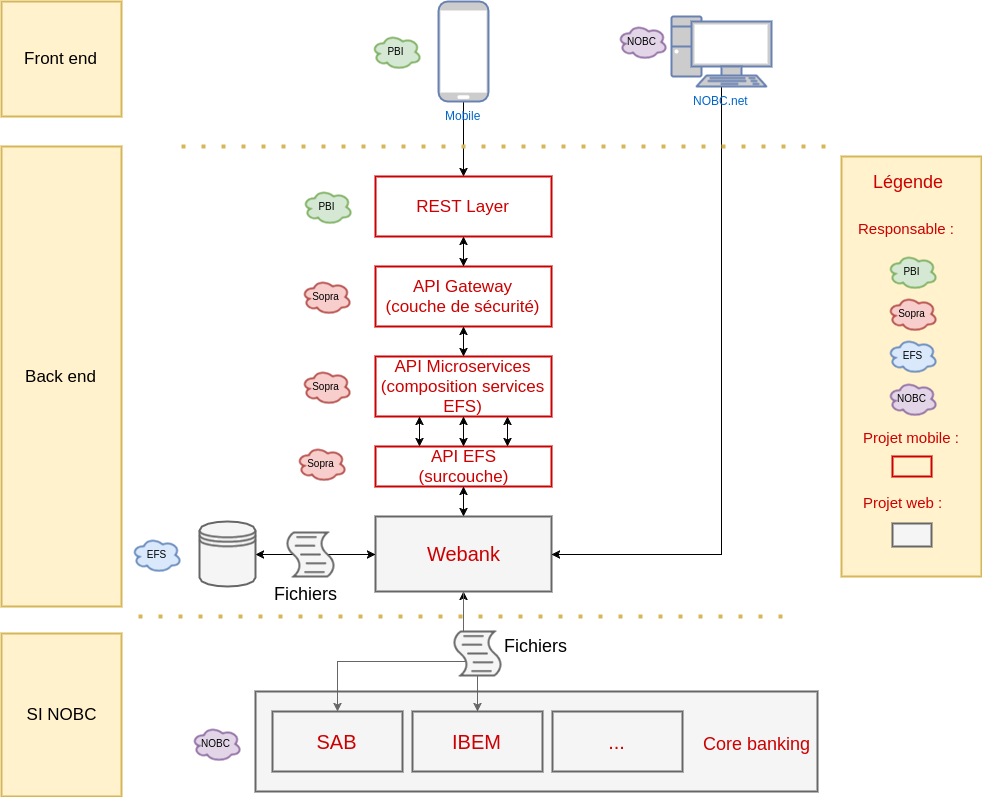
\includegraphics[scale=0.45]{images/travailNeuflizeOBC/architecture/archiFonc.png}
	\centering
	\caption{Présentation du projet et des acteurs}
	\label{archiFonc}
\end{figure}
	
\section{Architecture de l'application}
	\paragraph{}
Dans cette partie nous allons présenter plus en détails l'architecture globale du projet d'application mobile de Neuflize OBC. Comme nous l'avons vu précédemment, ce projet est basé sur une architecture multicouches dont la structure est représentée dans sa globalité en annexe \ref{a2}. Nous allons maintenant décrire chacune des couches afin de comprendre le fonctionnement du projet. Cependant, les technologies employées étant nombreuses, il serait peu pertinent de toutes les expliciter, ainsi seul l'essentiel en lien avec le stage sera ici décrit. Toutefois, il est possible de retrouver toutes les briques en annexe.

\subsection{Axway API Gateway}
\label{axway}

	Deux instances de l'API Gateway d'Axway ont été installées en mode « actif/actif » afin d'assurer la mise en place de la couche \textit{security} et celle de la couche \textit{management}. La répartition de charge est gérée par l'instance positionnée en amont. \\
		
	L'API Gateway de la couche security est le serveur traitant les appels API. Cette dernière est en charge de la sécurité applicative des appels vers la couche API Management. Elle est positionnée dans le tier 1, reçoit les appels « HTTPS » et a principalement pour objectif d’effectuer les actions suivantes : \\
	
	\begin{itemize}
		\item Vérifier la validité des certificats partenaires
		\item Filtrer les requêtes entrantes 
		\item Agir comme un pare-feu applicatif afin de vérifier le contenu des messages REST
		\item Répartir la charge vers les composants en aval
		\item Protéger le SI en limitant le nombre d’appels API via un mécanisme de régulation du traffic et en limitant le nombre d'appels au SI via un mécanisme de cache \\
	\end{itemize}
	
	La couche API management, dans le tier 2, permet de configurer et d’exposer les API. Elle assure les fonctionnalités suivantes : \\
	
	\begin{itemize}
		\item Publier et sécuriser les API
		\item Gérer le cycle de vie des API
		\item Gérer l’authentification et les habilitations (développeurs et administrateurs API)
		\item Embarquer les développeurs d’applications consommatrices d’API
		\item Auditer, suivre la consommation des API, gérer les quotas
		\item Assurer la haute disponibilité \\
	\end{itemize}
	
	Une interface web avait aussi été mise à notre disposition par Axway, nous permettant de traquer toutes les requêtes effectuées. \\
	
	Afin d'assurer la sécurité l'API management utilise \textit{OAuth2} ainsi que \textit{JWT}. OAuth2 est un framework d'authentification permettant d'authentifier plusieurs applications différentes. JWT est un protocole d'authentification permettant de créer et valider des \textit{tokens} (ou jetons) de sécurité. Ces tokens sont ensuite utilisés pour limiter l'accès des utilisateurs aux API. Pour chaque utilisateur qui se connecte, la Rest Layer envoie une assertion SAML. Si cette assertion est vérifiée par l'API management un token est généré contenant les informations permettant à un utilisateur d'accéder aux ressources protégées. Ainsi, toute les requêtes émises vers l'api microservices doivent contenir un token permettant l'authentification sans quoi elles seront rejetées (erreur 401 : Unauthorized). J'ai simplifié ici la procédure et limité les informations à ce qui est nécessaire pour la compréhension du rapport. En effet, celle-ci est extrêmement complexe et dépasse ce qui a été effectué dans le cadre du stage.
	
\subsection{Microservices}

	Avant d'aller plus loin, nous allons expliciter ce qu'est une architecture microservices \cite{bib_microservices} afin de pouvoir comprendre la structure des API. Il s'agit d'un paradigme d'architecture qui jouit actuellement d'une grande popularité aux dépends de celles plus classiques (N-tiers, SOA...), inventée afin de répondre aux problématiques soulevées par les projets de grande ampleur. \\
	
	Cette approche consiste à développer une application sous forme d'un ensemble de services dont la granularité correspond à une fonctionnalité élémentaire en terme métier. Chacun de ces services doit posséder son propre contexte d'exécution et ainsi être testable et déployable indépendemment en favorisant un couplage le plus faible possible. Ils peuvent être écrit dans des langages différents et communiquer entre eux via, par exemple, le protocole HTTP et la mise en place d'une API REST, ce qui est le cas pour ce projet. On parle alors de microservices, terme qui s'oppose aux applications plus classique que l'on dit monolithiques.\\
	
	Les applications d'entreprises classiques sont très souvent construites sur une architecture trois tiers constituées de trois parties majeures :
	\begin{itemize}
		\item Une interface client permettant la présentation des données
		\item Un serveur contenant la logique métier et effectuant le traitements des données
		\item Une couche d'accès aux données permettant de gérer les données persistantes \\
	\end{itemize}
	
\begin{figure}[h!]
	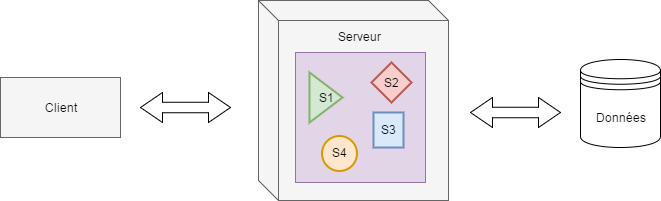
\includegraphics[scale=0.5]{images/travailNeuflizeOBC/architecture/troisTiers.png}
	\centering
	\caption{Architecture trois tiers monolithique}
	\label{troisTiers}
\end{figure}
	
	L'ensemble des services est contenu dans la même application et ces derniers sont donc exécutés dans un même processus. Ainsi, le moindre changement nécessite de rebuild et redéployer l'application entièrement. La scalabilité horizontale (par exemple un ajout de serveur) en est impactée. En effet, l'application entière doit être migrée si l'on souhaite changer de matériels afin d'améliorer les performances. Si un certain module est plus lent, il n'est pas possible de le déplacer indépendemment afin d'améliorer son exécution, il faut répliquer le monolithe entier tandis que du côté des microservices il est possible de répliquer un service en particulier et d'en redéployer un sans avoir à redéployer tout l'ensemble. De plus, dans les gros projets, la quantité de code a tendance à augmenter rapidement impliquant une hausse de la compléxité et rendant ainsi difficile l'ajout de nouvelles fonctionnalités. Le couplage entre ces dernières devient fort et les nombreux effets de bords résultant de chaque modifications rendent alors l'application moins fiable, limitant les perspectives d'évolution.

\begin{figure}[h!]
    \begin{minipage}{.5\textwidth}
    \raggedright
		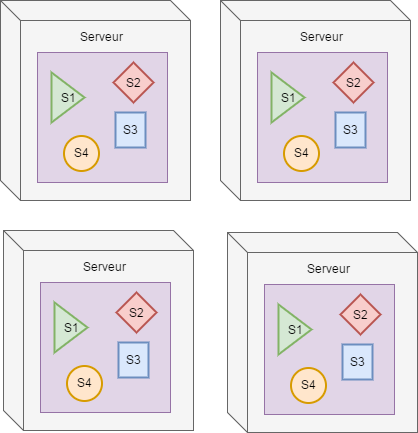
\includegraphics[scale=0.55]{images/travailNeuflizeOBC/architecture/monolithScale.png}
		\caption{Scalabilité horizontale d'une application monolithique \\}
		\label{monolithScale}
    \end{minipage}%
    \hspace{0.5cm}
    \begin{minipage}{.5\textwidth}
        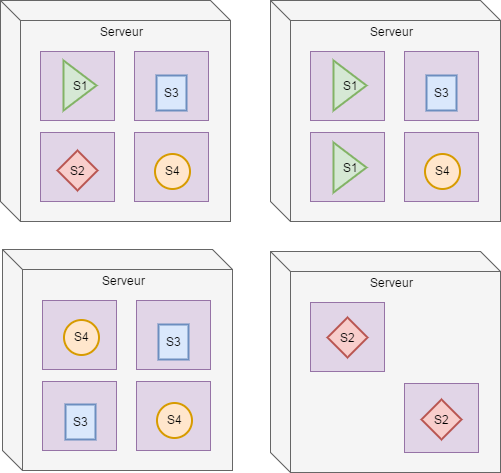
\includegraphics[scale=0.5]{images/travailNeuflizeOBC/architecture/microservicesScale.png}
		\caption{Scalabilité horizontale des microservices \\}
		\label{microservicesScale}
    \end{minipage}
\end{figure}

		Dans notre cas, l'objectif de la couche microservices , située dans le tiers 2, est de réaliser la composition des services métiers exposés par EFS dans le but d'exposer les données pour les applications ou les partenaires (comme PBI dont nous avons parlé dans la partie \ref{prezAppNeuflize}) qui viendront les consommer. Cette dernière est constituée des éléments présents sur la figure \ref{coucheMicroservices}. Les services EFS sont exposés via une surcouche API, située dans le tiers 2. \\

\begin{figure}[h!]
\raggedleft
	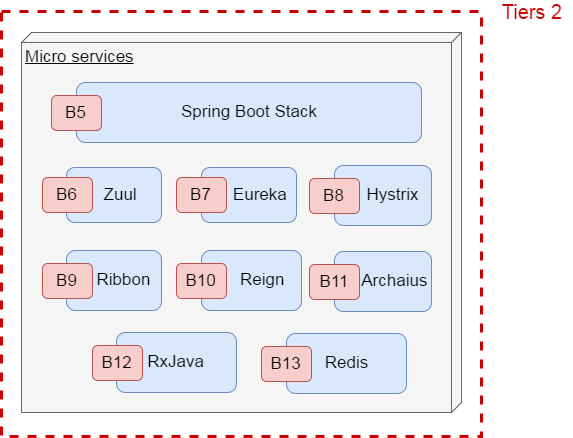
\includegraphics[scale=0.5]{images/travailNeuflizeOBC/architecture/coucheMicroservices.png}
	\centering
	\caption{Couche microservices}
	\label{coucheMicroservices}
\end{figure}
	
	\textit{Spring Boot Stack} est la brique applicative hébergeant les microservices. C’est dans cette dernière que la composition de services EFS est réalisée. Spring boot permet d'utiliser le framework java \textit{Spring} en simplifiant grandement la configuration, le déploiement ou encore la sécurité et en créant des applications cloud-ready.
	Cette brique prend aussi en charge l’implémentation des principaux patterns à savoir : \\
	
\begin{itemize}
	\item Circuit breaker : Capacité du système à être tolérant à la panne. En cas d’erreur successive lors de l’appel d’un sous-composant, le circuit d’appel est coupé « temporairement » en adoptant un comportement par défaut. L'implémentation qui a été choisie pour ce pattern est Hystrix de la stack \textit{Netflix OSS} \cite{bib_hystrix} permettant de contrôler la latence et les erreurs dues à des appels réseaux. L'idée essentielle est d'empêcher les erreurs en cascade dans un environnement distribué. Hystrix permet de \textit{fail-fast} mais de se rétablir rapidement créant ainsi une architecture tolérante aux erreurs capable de se remettre de manière autonome (on parle de self-heal). Ainsi, dès sa conception, le système prévoit les pannes.
	\item Feature toggle : Le principe est d’avoir une branche de développement et de déployer en production en continu. Ensuite, l’activation d’une « feature » est pilotée par le business. Cela permet aussi d’activer une fonctionnalité en fonction d’une population ou une stratégie particulière. \\
\end{itemize}

	Le serveur d'annuaire, essentielle à une architceture distribuée, permet la détection automatique des instances déployées. Les instances des applications sont accédées via leur nom (par exemple account-service) plutôt que par leurs adresses physiques/IPs. Les applications n'ont plus besoin de connaitre les adresses des instances. L'implémentation de l'annuaire de service est Eureka de la stack \textit{Netflix OSS} \cite{bib_eureka}. Les applications clientes peuvent s'enregistrer sur Eureka, via une annotation, qui fournira des metadatas telles que l'URL, le port ou encore le fil de vie (healthcheck) des instances. Eureka reçoit des messages dits "heartbeat" provenant de ces applications, si aucun message n'est reçu, en fonction d'un temps configurable, il supprimera l'instance. \\

	Ensuite, le point d'entrée unique de l'architecture microservices est sa gateway fournissant des services de routage dynamique, surveillance, résilience et sécurité. L'implémentation choisie est Zuul de la stack \textit{Netflix OSS} \cite{bib_zuul}. L'affichage d'une page web ou mobile peut nécessiter l'appel à une dizaine de microservices différents. Il n'est pas envisageable pour l'application cliente de connaitre l'ensemble des adresses physiques des microservices. Pour répondre à cette problématique, la gateway devient la seule adresse à connaitre pour les applications clientes. Zuul est aussi utilisé pour router les requêtes vers les services adéquats. Celui-ci retrouve les adresses des services automatiquement en interrogeant Eureka. Cependant, les services EFS et d'authentification (Axway gateway) sont paramétrés manuellement puisqu'ils ne sont pas enregistrés sur Eureka. La charge sera ensuite répartie grâce à un autre outils de Netflix, Ribbon, qui fourni des fonctionnalités de load-balancing permettant de distribuer la charge de travail. \\
	
\section{Premiers travaux}
	\input{src/travailNeuflizeOBC/premiersTravaux}
	
\section{Tests fonctionnels}
		Nous allons, dans cette partie, décrire les travaux concernant la mise en place d'une procédure complète permettant de gérer et réaliser des tests fonctionnels de manière automatique et fournissant des rapports complets pouvant être remis au client.

\subsection{Enjeux et spécifications}
		Comme nous l'avons vu précédemment, les services de nos API rest sont destinés à être consommés par PBI, en charge du développement de la partie frontend de l'application mobile. Ainsi, nous étions souvent en contact avec ces derniers afin de prendre connaissance des différentes anomalies liées à nos services et de pouvoir répondre à l'évolution de leur besoins. Après correction de celles-ci, il était fréquent que nous soyons amenés à livrer la nouvelle version des services. Ces livraisons permettaient à PBI de pouvoir continuer le développement de l'application dans les meilleures conditions possibles. Elles s'effectuaient sur deux environnements différents à savoir \textit{homo3} et \textit{rgb} comme il est possible de l'observer sur la figure \ref{environnement}. \\
	
	L'environnement homo3 est un serveur d'homologation sur lequel était effectué les recettes avec le client. Celui-ci permet de réaliser des tests afin de s'assurer que le produit est conforme aux spécifications. L'environnement rgb est un serveur de pré-production dont la structure, contrairement à homo3, est identique à celui de la production. Ce serveur permet de réaliser un béta test du produit ainsi que des tests de charge par le client dans des conditions réelles afin de déceler les derniers bug potentiels avant la mise en production. De son côté, PBI, possède la même structure avec un serveur de recette nommé \textit{ST} et un environnement de pré-production nommé \textit{ET} connectés à nos environnements. Ainsi, nous partagions les mêmes données pour réaliser nos tests (identifiants utilisateur, comptes bancaires, portefeuilles, positions, transactions...) Concernant les services EFS nous étions toujours sur leur production ou sur des mocks (objets simulés reproduisant le comportement d’objets réels) en attendant la mise en production des services demandés.\\
	
	Cependant, avant de procéder à la livraison des services sur ces environnements, il est nécessaire d'effectuer une batterie de tests fonctionnels permettant de vérifier que le comportement des API est conforme aux spécifications. Ces tests sont essentiels à la satisfaction client et permettent de gagner un temps précieux en évitant d'attendre les retours avant d'identifier les possibles anomalies. Nous réalisons beaucoup d'évolutions et de corrections de bugs qui parfois impliquent des effets non désirés qui peuvent être décelés par de tels tests. Néanmoins, dans notre cas, peu de ces tests avaient été mis en place et il n'existait aucune procédure à suivre. Les cas de tests était rédiger sous Word et le résultat de leur exécution était consigné dans des fichiers excel, peu lisibles, contenant peu d'informations et difficilement traçables. De cette manière, il est difficile de normaliser l'écriture des tests et la création d'un rapport est chronophage (créer les formules excel, etc...) pour un résultat qui ne sera pas exhaustif. En outre, il est impossible d'avoir une vue d'ensemble sur l'évolution des tests au cours du temps et est compliqué de suivre l'état d'une spécification particulière à différentes dates données. Par ailleurs, le client lui-même a souhaité un autre format plus rigoureux permettant de vérifier le comportement des services dans leur intégralités et de pallier aux inconvénients que nous avons cité. \\	
	
\begin{figure}[h!]
	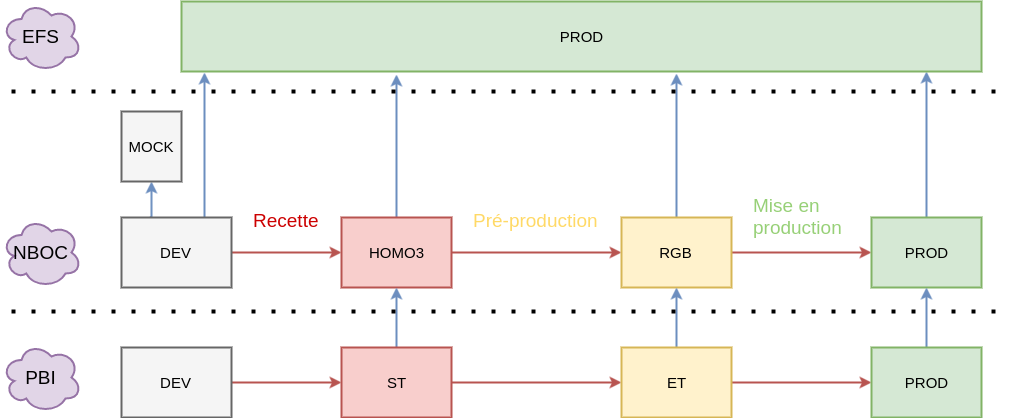
\includegraphics[scale=0.5]{images/travailNeuflizeOBC/testsFonc/environnement.png}
	\center
	\caption{Environnements}
	\label{environnement}
\end{figure}

	Ainsi, j'ai été chargé de mettre en place une procédure pouvant répondre à ce besoin. Cette dernière devait :	
	\begin{itemize}
		\item définir les cas de tests
		\item fournir des rapports d'exécution de tests détaillés
		\item nécessiter peu de développement, il était en effet inutile de réinventer la roue
		\item être gratuite
		\item être accessible à tout moment à n'importe quel membre de l'équipe de développement qui pourrait être amené à effectuer une livraison \\
	\end{itemize}
	\label{testsFonc_01}

\subsection{TestLink : Un gestionnaire de tests}
		Dans le but de répondre aux besoins explicités précedemment, j'ai décidé d'avoir recours à un gestionnaire de tests sous forme d'une application web. En effet, celle-ci pourrait être mise en place sur un seveur interne et rendue disponible pour toute l'équipe, favorisant ainsi le partage d'information et permettant de centraliser toutes les données concernant la réalisation des tests fonctionnels, assurant ainsi un versionning cohérent. De plus, cela répond à la problématique de mise en place rapide et de maintenabilité efficace (pas de mise à jour à gérer sur tous les postes, etc...). \\
	
	Après avoir mené plusieurs recherches, j'ai pu constater qu'il existait différents gestionnaires open-source concurrents sur le marché répondant à nos exigences : \textit{Salomé TMF}, \textit{TestLink} ou encore \textit{Squash TM}. En effet, ces derniers nous offrent tous la possibilité de créer des tests, de les lier aux exigences client ou encore de créer des campagnes de tests puis d'exporter les résultats sous forme de rapport détaillé. Ces outils proposant des fonctionnalités très proches, j'ai décidé d'en choisir un disposant d'une grande flexibilité ainsi que d'une communauté active afin de pouvoir faciliter l'adaptation à nos cas de tests. En effet, les gestionnaires génèrent des rapports regroupant des informations telles que la description des tests, leur temps d'exécution ou leur status. Cependant, dans notre cas, nous souhaitions pouvoir inclure pour chacun des tests des informations supplémentaires telles que le nom du service auquel appartient la fonctionnalité testée, l'identifiant de l'utilisateur utilisé pour le test, le numéro de compte bancaire utilisé et de manière générale, tous les paramètres utilisés pour réaliser la reqûetes testées. PBI partageant les mêmes données que nous sur les environnements d'homologatoin et de pré-production, il leur était alors possible de vérifier de leur côté que les tests passent effectivement. De plus, lorsqu'ils remarquaient une anomalie, ils pouvaient nous transmettre les paramètres qu'ils avaient utilisé afin que nous puissions reproduire celle-ci chez nous. \\
	
	Ainsi, j'ai décidé d'utiliser l'outil \textit{TestLink} dont la communauté avait mis à disposition de tous des templates permettant de modifier le code source afin de customiser la génération des rapports de tests. Celui-ci est une application web développée en PHP et utilisant le système de gestion de base de données MySQL. Il permet de centraliser toute la gestion des tests fonctionnels du projet en les organisant par le biais des structures présentées dans le tableau \ref{structuresTestlink}.

\begin{table}[h!]
	\center
	\begin{tabular}{| c | c |}
     \hline
     Cas de test & Test fonctionnel définissant un scénario spécifique \\ \hline
     Suite de tests & Collection de cas de test validant une même fonctionnalité \\ \hline
     Plan de tests & Collection de suite de tests contenant toutes les informations \\  & telles que la portée, les étapes, la version etc...\\ & Un plan est exécuté pour un build particulier \\ \hline
     Build & Une release spécifique des APIs testées \\
     \hline
	\end{tabular}
	\caption{Structures fournies par TestLink}
	\label{structuresTestlink}
\end{table}

Cet outil présente de nombreux avantages qui m'ont conforté dans mon choix :
\begin{itemize}
	\item Campagnes de tests versionnées dont l'historique est enregistré en base de données.
	\item Export et import de cas de test et de leur résultats
	\item Connection avec \textit{Mantis}, un tracker de bug utilisé dans notre projet
	\item Gestion de rôles sur les tests (qui effectues le test, qui valide etc...)
	\item Rapport complet dans différents formats
	\item Accessible à toute l'équipe n'importe quand 
	\item Simplicité d'utilisation et de mise en place \\
\end{itemize}

	Ensuite, avant de procéder à la création des cas de test sur TestLink, j'ai commencé par définir la structure du futur plan de test qui serait exécuté avant chaque livraison. Ainsi, j'ai décidé de séparer l'ensemble des tests en deux grandes familles : ceux concernant les fonctionnalités de consultation et ceux concernant les fonctionnalités de transaction, ce qui m'amena à la création de deux suites de tests. Après cela, j'ai créé autant de suites de tests qu'il y avait de fonctionnalités décrites dans l'annexe \ref{a2}. Il est possible d'observer sur la figure \ref{testlink} l'organisation d'un plan de test type. Afin de garder le même formalisme tout le long de la réalisation des plans de tests et pour assurer une certaine cohérence, j'ai décidé de mettre en place plusieurs conventions définissant une stratégie de test :
	
	\subsubsection*{Cas de test}
	Les cas de tests doivent avoir un nom de la forme [id]-[titre] où
	\begin{itemize}
		\item id désigne un ID unique permettant de les identifier rapidement et de faciliter leur organisation. Celui-ci est \textit{NOBC-API-XX}, où XX représente le numéro du test. 
		\item titre désigne de manière clair et concise l'objectif du test
	\end{itemize}		
	De plus, chaque cas de test possède en attribut un numéro de version de la forme \textit{vX} où X est incrémenter de 1 chaque fois que le cas de test est modifié.
	
	\subsubsection*{Plan de test}
	Les plans de tests doivent avoir un nom de la forme [scope]-[environnement]-[version] où
	\begin{itemize}
		\item scope désigne la portée du plan de test : "complete" pour tous les tests, "transaction service" pour les tests du service de transaction, "transaction overview" pour les tests de la fonctionnalité transaction overview etc...
		\item environnement désigne le serveur sur lequel sont effectués les tests : homo3 ou rgb
		\item version est de la forme vX.Y.Z où
			\begin{itemize}
				\item X est incrémenté de 1 lorsqu'un nouveau cas de test est ajouté ou supprimé du plan
				\item Y est incrémenté de 1 lorsqu'un cas de test existant du plan a été modifié
				\item Z est incrémenté de 1 à chaque exécution du plan
			\end{itemize}
	\end{itemize}
	
	\subsubsection*{Build}
	Les builds doivent avoir un nom de la forme : [version] où
	\begin{itemize}
		\item version désigne la version de l'API microservices testée \\
	\end{itemize}

	La stratégie de test étant définie, il fallait maintenant déterminer quelles informations devaient être transmises au sein des rapports de tests. Les gestionnaires de tests proposent de remplir des formulaires afin consigner le résultat des tests une fois ceux-ci effectués, ce qui servira par la suite à générer un rapport. Cependant, ces derniers sont plutôt génériques et ne permettent pas de renseigner des données spécifiques à un projet particulier. Comme nous l'avons dit plus haut, nous souhaitions être en mesure de passer des paramètres supplémentaires afin de faciliter nos échanges avec PBI, comme : \\
	
	\begin{itemize}
		\item url et paramètres utilisés pour la requête
		\item service testé
		\item identifiants utilisés
	\end{itemize}
	
	\begin{figure}[h!]
	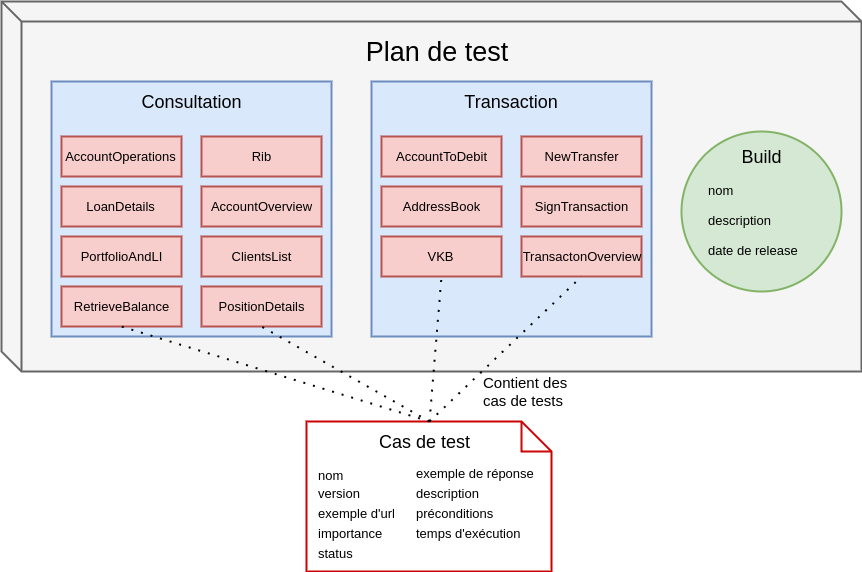
\includegraphics[scale=0.5]{images/travailNeuflizeOBC/architecture/testlink.png}
	\centering
	\caption{Configuration d'un plan de test type}
	\label{testlink}
\end{figure}
	
	Ainsi, j'ai décidé de modifier le code source de TestLink afin de rajouter les champs dont nous avions besoin aux formulaires de tests. J'ai réalisé cette modification en deux étapes dont la première consistait à ajouter les champs aux formulaires puis à gérer la partie front en PHP. La seconde concernait la récupération des données et leur sauvegarde en base de données, ce qui a impliqué la création de nouvelles requêtes SQL. Une fois les champs mis en place, j'ai créé un cas de test puis générer un premier rapport au format PDF en guide de POC (proof of concept). Celui-ci ayant été jugé satisfaisant, j'ai dû étudier l'ensemble des spécifications du projet concernant chacun des services mis en place afin de procéder à l'écriture de tous les cas de tests. Cela m'a permis de mieux comprendre le besoin du client, d'avoir une bien meilleure vision sur le projet dans sa globalité en m'apportant des informations sur l'utilité de chaque service et de pouvoir me former sur le projet en restant productif.
	
	Ces cas de tests permettaient de vérifier que les réponses des requêtes émises vers l'API microservices étaient en accord avec les attentes de PBI. Par exemple, les réponses étant au format JSON, ils permettaient la vérification de la présence de tous les champs obligatoires, la cohérence des valeurs des champs (\hl{TODO exemple a prendre dans la spec}) ou encore la vérification de la cohérence des données de notre backend avec celles de l'application web.
	\label{testsFonc_02}
	
\subsection{Rapports de tests obtenus}
		Une fois tous les cas de tests rédigés, j'ai procédé à la réalisation d'une campagne de tests complète aboutissant à la génération d'un rapport. Afin de procéder à cela, pour chacun des tests j'ai utilisé l'outil \textit{Postman} qui est une plateforme proposant une interface graphique facilitant la construction de requêtes. Cet outil est conçu pour faciliter le développement des APIs en permettant de les intéroger de manière très rapide et simple sans avoir à développer un client pour les consommer. Dans l'optique de mettre à profit les tests effectués, nous avons connecté TestLink à Mantis, une application web permettant d'assurer le suivi des anomalies dans laquelle il est possible d'ouvrir des tickets concernant des bugs qui seront alors pris en charge par les développeurs jusqu'à leur clôture. Ainsi, lorsqu'un test échouait il était possible, d'un simple clique sur TestLink, de générer automatiquement un ticket sur Mantis avec toutes les informations rajoutées précédemment. Les développeurs avaient donc toutes les données (url, service etc...) pour reproduire l'anomalie en locale et la corriger. \\
	
	TestLink permet de personnaliser la génération des rapports de tests après l'exécution d'un plan complet. De plus, il est possible de générer le rapport dans différents formats. Nous avons donc décidé que chaque livraison comporterait un rapport complet contenant toutes les informations au format PDF. Cependant celui-ci pouvant être très conséquent, nous avons choisi de l'accompagner d'un rapport léger généré au format excel ne contenant que le nom des tests et leur statut (succès, echec, bloqué) avec un code couleur permettant a PBI de rapidement repérer les tests en échec et leur nombre. Ces derniers ont déclaré être très satisfait des nouveaux rapports fournis, c'est pourquoi il a été décidé que l'exécution des tests fonctionnels sur la plateforme TestLink serrait obligatoire avant chaque livraison. En attendant l'attribution d'un serveur pour héberger le gestionnaire de test, celui-ci a été mis en place sur le serveur personnel d'un des architecte du projet afin de le rendre accessible à toute l'équipe. \\
	
	La réalisation de ces tests et leur exécution m'a permis de relever certains écarts entre le produit réalisé et les spécifications. Par exemple \hl{TODO : exemple d'ecarts loanDetails}. C'est pourquoi, après avoir centralisé tous les écarts que j'avais relevé, j'ai organisé une réunion avec mon chef de projet ainsi que certains développeurs dans le but de déterminer lesquels pourraient être corriger et lesquels ne le pourraient pas, nécessitant de prendre contact avec le client afin de clarifier la situation. Au terme de cette réunion, j'ai pu créer une nouvelle version des spécifications afin de les mettre à jour puis j'ai fait part de ces modifications à PBI à travers des mails rédigés en anglais. Ensuite, la mise en place de ces outils a permi à l'équipe de pouvoir effectuer les livraisons dans de meilleurs conditions puisque les anomalies pouvaient être détectées avant d'attendre les retours du client. De plus, tous les tests étaient centralisés, organisés et pouvaient être exécutés en parallèle par différentes personnes ce qui permettait un gain de temps à la fois sur l'exécution des tests mais aussi sur leur gestion (archivage, formalisme, perte de documents etc...). \\
	
	Néanmoins, afin d'exécuter les tests, les développeurs utilsaient Postman pour construire et envoyer les requêtes. Si cet outil est extrèmement utile pour développer un nouveau service ou tester un nouveau endpoint lors du développement, il n'est pas conçu pour exécuter un grand nombre de requête les unes après les autres à des fins de tests. En effet, comme nous l'avons expliqué dans la partie \ref{axway} les requêtes doivent posséder un token d'authentification dans leur header pour espérer passer la gateway et atteindre la couche microservices. Or, pour cela, il est nécessaire d'envoyer, toujours avec Postman, une requête de génération de ce token à l'API gateway. Après cela, il faut se connecter sur l'interface web fourni par Axway, retrouver la requête ainsi que sa réponse et copier le token. Cependant, pour accéder à cette interface il faut d'abord être en mesure d'accéder à l'environnement testé, Homo3 ou RGB, qui, rappelons le, n'ont pas les mêmes instances de l'API Gateway et ne sont pas accessibles de l'extérieur. Pour cela, il faut se connecter en RDP sur TSE puis ensuite utiliser les bonnes adresses et identifiants pour accéder à l'interface désirée. De retour sur Postman, il faut coller le token dans le header de la requête que l'on souhaitais tester. Cette démarche est illustrée sur l'annexe \ref{a3} qui décrit la procédure d'authentification gérée par la gateway. Et il faut répéter cette démarche \textbf{à chaque fois que le token expire}, ce qui ne pose pas de problèmes lorsque l'on souhaite envoyer une requête pour tester son code mais devient rapidement très fastidieux lorsque l'on a des centaines de requêtes à envoyer pour exécuter tous les tests. 
	Un exemple classique serait de tester le service de \hl{TODO : exemple avec buloc}
	
	Il résulte de cela une perte considérable de temps qui aurrait pu être mis au profit du développement, de l'amélioration des points jugés sensibles ou encore de la correction des anomalies. En effet, il n'était pas rare que l'ensemble des tests puissent occuper une personne presque \textbf{une demi journée}, ce qui se révèle être énorme sur des sprints de deux ou trois semaines. Il fallait donc trouver le moyen de conserver la procédure de test et la génération de rapports tout en réduisant drastiquement le temps que cela demandait, c'est pourquoi nous avons décidé d'automatiser les tests fonctionnels.
	
	
	\label{testsFonc_03}

\subsection{Automatisation des tests fonctionnels}
		La fin de la phase de développement approchant, l’équipe avait fait ressentir le besoin de procéder à la réalisation de tests de charge afin de vérifier la capacité des APIs à soutenir le trafic attendu. Pour cela, l’un des outils open source les plus performant et rapide à mettre en place du marché est \textbf{Apache JMeter}. Ainsi, afin de centraliser tous les tests et de gagner du temps sur la formation aux outils et leur installation, j’ai décidé d’utiliser JMeter pour aussi automatiser les tests fonctionnels. \\
	
	Ce logiciel, développé en java avec l’API Swing par la fondation Apache, permet de réaliser aussi bien des tests de performance que de charge ou encore fonctionnel compatibles avec un grand nombre de protocoles et technologies. Il permet de créer des requêtes et de les exécuter de manière automatique sur des serveurs web, des base de données via JDBC, sur des LDAP et bien d’autres. Celui-ci exporte le résultat des tests au format XML ce qui permet aisément de les réimporter sous TestLink. En effet, ce dernier nous offre la possibilité d’importer les résultats de tests via des fichiers aussi au format XML. Ainsi, il était possible de jouer les tests automatiquement dans un premier temps sur JMeter puis de générer, dans un second temps,  un rapport à destination du client via TestLink. En outre, JMeter met à notre disposition de nombreux avantages : \\
	
\begin{itemize}
	\item Logiciel open source disponible gratuitement
	\item Interface en Swing très intuitive
	\item Multithreading permettant de simuler la concurrence des requêtes lors des tests de charges via la mise en place de différents groupes de threads représentant des utilisateurs fictifs
	\item Possibilité d’installer de nombreux plugins développés par une communauté active afin de customiser les tests si besoin est \\
\end{itemize}
 
	Il propose de construire les plans de tests de manière interactive en ayant recours à des composants préconçus qui interagiront entre eux. Il en existe différents types pouvant être utilisés comme nous le montre le tableau figure \ref{composantJMeter} : \\

\begin{table}[h!]
	\center
	\begin{tabular}{| c | c |}
     \hline
     Composant & Description \\ \hline
     Moteur d’utilisateurs & Il s’agit de l’élément qui définira le niveau de la charge à appliquer \\ & (nombre d’utilisateurs, d’itération, temps de montée en charge) \\ \hline
     Contrôleur logique & Permet de structurer les tests \\ \hline
     Configuration & Permet de définir les configurations communes à plusieurs éléments \\ \hline
     Compteur de temps & Permet de gérer le temps d’attente avant l’exécution d’un composant \\ \hline
     Echantillons & Réalise les opérations de tests (ici des requêtes HTTP) \\ \hline
     Pré-processeurs & Agi avant les échantillons pour réaliser des opérations \\ \hline
     Post-processeurs & Agi sur le résultat des échantillons \\ \hline
     Récepteurs & Traite et formatent le résultat des tests \\ \hline
     Assertions & Permet de vérifier le résultat des échantillons \\ \hline
	\end{tabular}
	\caption{Composants JMeter}
	\label{composantJMeter}
\end{table}
	
	Les tests étant nombreux, j’ai décidé de les classer par service afin de rapidement en retrouver un en particulier et de pouvoir les jouer selon le microservice désiré. Cela s'est avéré utile par la suite, lorsqu'un service était défaillant, pour pouvoir facilement lancer les tests le concernant, étudier les réponses obtenues et cibler l'origine des anomalies. Il était, en effet, beaucoup plus rapide d'avoir recours à JMeter qui permettait d'envoyer de nombreuses requêtes avec différents paramètres plutôt que d'exécuter des requêtes manuellement via Postman jusqu'à réussir à reproduire un bug pour l'analyser. 
	
	Après cela, j’ai défini la structure du plan de test général qui devais contenir tous les tests fonctionnels en choisissant les composants qui allaient le constituer puis en procédant au paramétrage des différents éléments de configuration. La capture d’écran de JMeter figure \hl{TODO ref} montre la structure que j’ai établi pour le plan de test final et chacun des services. Cet structure est explicitée sous cette figure via une explication du détail de chaque élément employé ainsi que ses intéractions avec les autres. \\
	
	\hl{FIGURE CAPTURE D'ECRAN JMETER}
	
	\paragraph{1 - Moteur d'utilisateur}
	Le moteur d'utilisateurs est l'élément englobant tous les composants, permettant de définir le niveau de charge affecté au plan de tests. Dans notre cas, ces derniers étant fonctionnels, le nombre de threads (utilisateurs) ainsi que le nombre d'itération des requêtes est de 1. De plus, le temps de montée en charge est laissé par défaut afin que les tests soient exécutés dans les meilleures conditions possibles.

	\paragraph{2 - Contrôleur logique}
	Les contrôleurs logiques permettent de définir la structure du plan de tests. Ici, il y en a un par service testé. Ils contiennent tous les tests d'un service particulier, les opérations à effectuer pour les mener à bien et les assertions.
	
	Par exemple, il y a le controleur NewTransfer regroupant les tests du service du même nom permettant de réaliser des transactions bancaires.
	
	\paragraph{2.1 - Echantillon}
	Les échantillons représentent les requêtes HTTP qui seront exécutées par JMeter. Afin de maintenir la cohérence avec TestLink, toutes les requêtes testées portent un nom de la forme NOBC-API-XX, ce qui correspond aux ID des cas de tests défini dans TestLink. Celles-ci sont alors vérifiées grâce à des assertions. Celles dont le nom n'est pas de cette forme ne sont pas vérifiées et n'ont pas d'assertions, elles ne sont exécutées que pour remplir les préconditions nécessaires à l'exécution des tests.
	
	Par exemple, pour pouvoir appeler le service NewTransfer, il faut l'identifiant d'un compte débiteur et créditeur, et comme pour tout service il faut un token d'authentification. Ainsi, il faut donc au minimum appeler les services AccountToDebit, Addessbook et TokenInfo, extraire les informations souhaitées puis les utiliser en paramètre de la requête vers NewTransfer.
	
	De manière générale, toutes les requêtes testées seront toujours au minimum précédée d'une requête de précondition permettant de générer le token d'authentification. Il s'agit de la raison majeure pour laquelle JMeter a permi un gain de temps considérable, il n'y avait en effet plus à se soucier d'aller chercher un token en passant par le TSE à chaque exécution de requête.
	
	\paragraph{2.2 - Json extractor}
	Cet élément est de type post-processeur et permet d'extraire la valeur d'un champ d'une réponse au format JSON en utilisant JsonPath, un langage permettant d'adresser une partie d'un document JSON, puis de la stocker dans une variable globale. Positionné dans un échantillon de type précondition, il permet d'extraire une information qui pourra ensuite être passée en paramètre d'une requpete testée.
	
	Par exemple, après l'appel à AccountToDebit, il permet de récupérer l'identifiant d'un compte débiteur qui sera utilisé comme paramètre dans la requête NOBC-API-28 vers NewTransfer.
	
	Cet élément est aussi utilisé sur les requêtes testées pour extraire les valeurs de tous les champs de la réponse afin qu'ils soient ensuite vérifiés par le biais d'assertions.
	
	\paragraph{2.3 - Beanshell extractor}
	Cet élément a le même objectif que json extractor mais utilise un script Beanshell à la place de JsonPath. Beanshell est un langage de script dont la syntaxe est très proche de Java, interprété et dynamiquement typé. JsonPath permet d'accéder à un champ JSON particulier mais ne permet pas de stipuler des conditions complexes, c'est pourquoi dans certains cas j'ai dû recourir à des scripts Beanshell pour récupérer une valeur bien précise dans un champ d'une réponse.
	
	Par exemple, supposons maintenant que l'on souhaite appeler le service NewTransfer. Il faut dans un premier temps récupérer l'id d'un compte débiteur via un appel à AccountToDebit, ce qui est faisable facilement via JsonPath. Ensuite, il faut récupérer un compte créditeur via un appel à AddressBook. Or, le compte créditeur doit obligatoirement être différent du compte débiteur, condition qu'il n'est pas possible de préciser via JsonPath, c'est pourquoi il faut recourir ici à un script Beanshell pour récupérer une valeur cohérente.
	
	\paragraph{2.4 - Assertion}
	Les éléments assertions sont aussi de type post-processeur et sont des scripts Beanshell dont l'objectif est de vérifier des conditions puis de retourner une réponse qui déterminera le status du test après son exécution (succès ou échec). Lorsque la requête à tester est exécutée, les éléments json extractor stockent les valeurs des champs de la réponse dans des variables qui pourront ensuite être utilisées dans ces scripts. Il ne reste plus qu'à écrire le script et les conditions de son succès/échec.
	
	\paragraph{2.5 - HTTP cookie manager}
	Elément de type pré-processeur permettant de configurer les cookies d'une requête avant son exécution. Ici, chaque requête doit au minimum posséder un cookie contenant le token d'authentification qui est récupéré automatiquement au préalable via l'exécution d'une requête permettant de générer ce dernier.
	
	\paragraph{2.6 - HTTP header manager}
	Elément de type pré-processeur permettant de configurer le header de la requête si besoin est. (par exemple le content-type)
	
	\paragraph{3 - View result tree}
	Elément permettant d'afficher, entre autre, le résultat de l'exécution de toutes les requêtes (succès/échec) ainsi que leur réponse. Celui-ci permet aussi de spécifier si l'on souhaite exporter le résultat du plan de test, les informations à exporter et leur format. J'ai décidé d'exporter les données au format XML afin de pouvoir les réimporter par la suite sous TestLink.
	
	\paragraph{4 - Summary report}
	Rapport permettant de fournir des informations plus détaillées sur l'exécution des tests comme le temps moyen par requête, le nombre de succès/échec, la bande passante consommée etc...
	
	\paragraph{5 - HTTP request defaults}
	Permet de configurer les paramètres HTTP par défaut (nom de domaine, port) ainsi que les informations concernant le proxy interne.
	
	\paragraph{6 - Users variables}
	Permet de définir des variables globales qui pourront être accessible depuis n'importe quel endroit. Une seule variable a été défini, il s'agit du nom de l'environnement sur lequel les tests devaient être effectués (Homo3 ou RGB). En effet, il serait extrêmement fastidieux de devoir changer l'url de toutes les requêtes manuellement à chaque fois que l'on change d'environnement ou de faire un deuxième plan de test, c'est pourquoi le nom de domaine de celui-ci a été externalisé dans une variable pouvant ensuite être appelée dans l'url de chacune des requêtes.
	
	\paragraph{7 - Assertions listener}
	Elément permettant d'afficher le résultat de toutes les assertions appliquées sur les requêtes exécutées dans le plan de tests. \\
	
	La structure du plan de test étant défini, j'ai ensuite procédé à l'écriture de toutes les requêtes, scripts Beanshell et autres assertions afin d'automatiser le plus de cas de test présent sur TestLink possible. Environ une centaine de ces cas ont pu être ainsi automatisés. Après l'exécution du plan de test dans son intégralité sur JMeter, un fichier XML contenant tous les résultats était généré. \\
	
	 Cependant, JMeter et TestLink étant deux outils totalement indépendants, il est évident qu'ils n'attendaient pas de fichiers XML ayant la même structure. Or, modifier ces fichiers manuellement serait contre productif et n'aurait alors aucun intérêt. Dès lors, j'ai décidé d'avoir recours au langage \textit{XSLT} ou \textit{eXtensible Stylesheet Langage Transformation}. Ce dernier, est un langage permettant de transformer un document XML en un autre en modifiant sa structure. Pour cela, il se base sur la manipulation de modèle ou template afin d'altérer le fichier XML source en remplaçant ses éléments d'origines par des éléments donnés. J'ai donc utilisé ce langage afin de construire des feuilles de style XSL dont l'objectif était de décrire les transformations à effectuer pour obtenir un fichier XML prêt à être importé sur TestLink à partir du fichier XML généré par JMeter. Afin d'appliquer cette feuille de style, j'ai mis en place un processeur XSLT nommé \textit{Saxon XSLT}. Celui-ci est un moteur prenant un document XSLT en entrée ainsi qu'un fichier XML source à transformer pour produire en sortie un nouveau document au format souhaité. Pour finir, j'ai mis en place un programme léger en Batch prenant en paramètre tous les documents impliqués ainsi que les données TestLink requises comme le titre du plan de test ou le nom du testeur et générant le fichier de résultat pour l'import.
	\label{testsFonc_04}
		
\subsection{Procédure finale et perspectives}
		Tous les éléments étant mis en place, j'ai rédigé un guide décrivant les actions à effectuer concernant les tests lors d'une livraison afin de générer les rapports à envoyer à PBI. Celui-ci décrit toutes les étapes pour la création ou modification des tests automatiques ainsi que le travail que j'ai effectué. De plus, celui-ci décrit comment installer et configurer l'ensemble des outils utilisés (TestLink, Apache JMeter et Saxon XSLT).
	
J'ai ensuite pu mettre le guide à disposition des développeurs et leur ai exlicité la marche à suivre finale qui est la suivante :
	\begin{itemize}
		\item Lancer les tests automatiques sur JMeter
		\item Récupérer le fichier XML généré contenant les résultats du plan de test
		\item Exécuter le programme Batch pour générer le fichier XML prêt à l'import pour TestLink
		\item Créer un nouveau plan de test sur TestLink
		\item Importer le fichier XML
		\item Repérer les tests en échecs et créer un ticket Mantis pour ces derniers
		\item Générer les rapports PDF et Excel \\
	\end{itemize}

\begin{figure}[h!]
	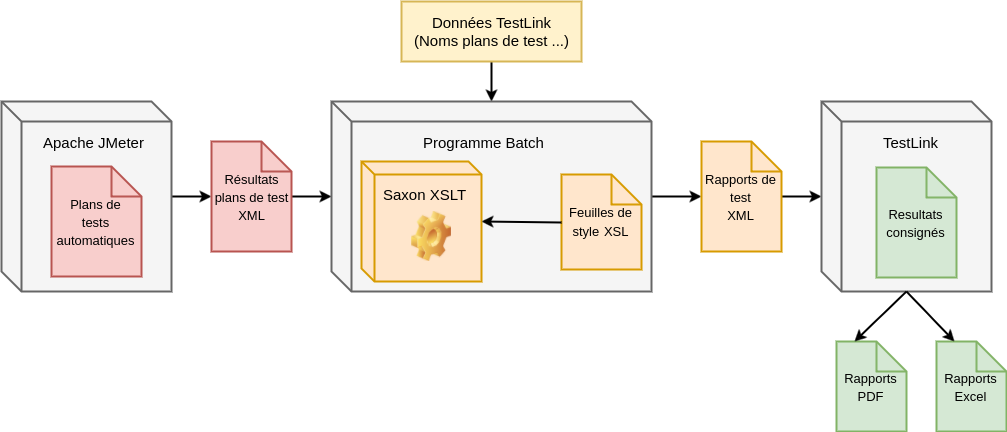
\includegraphics[scale=0.5]{images/travailNeuflizeOBC/testsFonc/testsProcedure.png}
	\centering
	\caption{Procédure de test finale}
	\label{testsProcedure}
\end{figure}

	Lors d'une livraison, une ressource pouvait parfois être occupé jusqu'à une demi-journée rien que pour exécuter l'ensemble des tests et consigner leur résultats, pour les raisons que nous avions évoquées partie \ref{testsFonc_03}. Avec cette nouvelle procédure, la génération des documents à destination du client prenait environ \textbf{10 minutes}, le plus long étant d'attendre la fin de l'exécution des tests automatiques. Ceci représente un gain de temps considérable pour l'équipe et permet d'obtenir des rapports conformes avec les besoins et attentes du client. De plus, cela a permis de soulager les développeurs d'un bon nombre de tâches répétitives et peu intéressantes d'un point de vue technique bien qu'essentielles dans le processus de satisfaction du client, dégageant ainsi du temps supplémentaire dans les sprints pour accomplir les objectifs fixés. \\
	
	Cependant, malgré les bénéfices apportés, certains points restent perfectibles. En effet, l'application web TestLink n'est pas actuellement hébergée sur un serveur dédié. Le projet touchant à sa fin, celui-ci sera repris par une équipe de maintenance qui aura besoin d'accéder à tous les outils et qui devra consigner les résultats de ses tests quotidiens c'est pourquoi il aurait été recommandé de pouvoir procéder à l'installation de TestLink sur un serveur dédié. 
	
	De plus, il aurait pu être intéressant de pousser l'automatisation des tâches à son maximum en ayant recours à Jenkins. En effet, il s'agit d'un outil d'intégration continue permettant d'automatiser différentes procédures. J'ai appris par la suite qu'un Jenkins aurait dû être mis en place au début du projet mais que cela n'avait pas été effectué faute de temps, il est prévu qu'un architecte se charge de cette installation. JMeter et TestLink sont tous deux compatibles avce cet outil tout comme les programmes Batch, il serait ainsi possible par la suite de programmer l'exécution des tests et la création des rapports de manière entièrement automatique à un intervalle de temps souhaité.
	\label{testsFonc_05}
	
\subsection{Aller plus loin : Tests de charge}
		L'équipe avait émis le besoin de mettre en place des tests de charge, JMeter étant installé et y étant formé j'ai pris en charge la réalisation de ces tests. Ces derniers consistent à mesurer le temps de réponse d'un système lorsque celui-ci est soumis à des conditions particulières afin de vérifier s'il est capable de soutenir le traffic attendu. Les conditions regroupent différents paramètres comme le temps de réponse, le volume du traffic, le nombre de requêtes effectuées en parallèle, la configuration du matériel ou encore la stabilité des serveurs. Afin de réaliser de tels tests, il faut dans un premier temps configurer l'environnement sur lequel ils seront exécutés. Dans notre cas, nous avions à notre disposition un environnement de pré-production (RGB) dont les caractéristiques étaient identiques à celles de la production, ce qui était approprié pour réaliser ce genre de tests. De plus, nous avions aussi l'environnement HOMO3 avec des capacités inférieures, idéal pour exécuter les tests dans des conditions un peu plus extrêmes dans le but mesurer la robustesse des APIs. \\
	
	Après cela, j'ai pris soin de définir différents scénarios de tests dont l'objectif étaient de simuler l'activité utilisateur afin de se rapprocher le plus possible des cas d'utilisation réels. Par exemple, un des scénario classique pourrait décrire la procédure suivie pour effectuer une transaction bancaire d'un compte vers un autre. Pour cela, l'utilisateur pourrait se connecter à l'application mobile puis initier sa transaction en choisissant des comptes débiteur et créditeur et il enfin il la signerait numériquement. De plus, celui-ci pourrait d'abord consulter ses comptes avant de prendre la décision de réaliser cette transaction. Les scénarios sont représentés par des diagrammes de cas d'utilisation comme celui présent sur la figure \ref{scenarioTest}, décrivant la réalisation d'une transaction. \\

	On peut ainsi remarquer rapidement les différents services (listés en annexe \ref{a2}) qui seront appelés lors de l'exécution de ce scénario :
	\begin{itemize}
		\item VKB pour générer le clavier virtuel permettant l'authentification et la signature de la transaction
		\item tokenInfo pour générer le token d'authentification
		\item newTransfer pour initier la transaction
		\item accountToDebit pour sélectionner le compte débiteur
		\item addressBook pour sélectionner le compte créditeur
		\item signByVKB pour signer la transaction
		\item clientList pour lister tous les comptes
		\item accountOverview pour consulter un compte particulier \\
	\end{itemize}
	
	Une fois les services identifiés, il ne restait plus qu'à construire le plan de test JMeter permettant de réaliser le scénario. Pour cela, j'ai réemployé la structure mise en place précédemment pour les tests fonctionnels. Cependant, j'ai supprimé l'ensemble des assertions puisque ces dernières peuvent influer sur les temps de réponse calculés par JMeter et n'ont pas d'intérêt dans un test de charge. Il ne restait donc qu'à modifier les scripts Beanshell déjà écrits pour les adapter à la situation. La principale différence réside dans la configuration du moteur d'utilisateur. En effet, sur les tests fonctionnels j'avais placé un tel moteur à la racine des plans afin qu'il englobe tous les composants. Ainsi, pour les tests de charges il suffisait de modifier les paramètres du moteur à savoir le nombre de thread, d'itération et le temps de montée en charge pour adapter les conditions d'exécution des scénarios sans avoir à modifier la structure des plans.
	
	Ces tests de charges ont par la suite été exécutés dans différentes conditions ce qui a permis de déceler certaines anomalies. \hl{TODO : exemple du probleme voir abdel}
	\label{testsFonc_06}
	
\section{Gestion des doubles relations}
	\subsection{Définition du besoin}	
	
	La version 1.0 de l’application mobile est réservée à la clientèle \textit{private} de NOBC, ne possédant que des produits de type PP (Personnes Physiques). Cependant, Neuflize ayant la volonté d'étendre la portée de ses services numériques afin de toucher un public toujours plus large, elle a souhaité rendre l'application disponible pour les PM (Personnes Morales). Ainsi, elle souhaitait inclure très rapidement dans une version 1.1 la clientèle \textit{double relation}, c’est-à-dire la clientèle de type "entreprise" mais qui dispose en même temps dans ses accès des produits "particuliers"; typiquement un entrepreneur qui en plus de ses comptes "entreprises" peut aussi voir/faire de la transaction sur ses comptes "privés". Or, d'un point de vue légal, les abonnés double relation n'ont pas les mêmes droits que les clients simple c'est pourquoi des modifications ont dû être apportées aux API. Les méthodes agiles nous apportant une certaine flexibilité, nous avons organisé une réunion avec les métiers afin d'étudier le besoin en détail et déterminer quelles modifications seraient appropriées. \\
	
	A l'issue de cette réunion avec le client, nous avons émis différentes problématiques afin de déterminer les actions à mettre en place au niveau de la couche microservices. Sur le site internet, un abonné double relation dispose d’un bouton lui permettant de visualiser soit ses comptes "entreprises" soit ses comptes "privés". Néanmoins, il n’est pas prévu à ce jour de tel bouton permettant à l’abonné de passer de ses comptes "entreprises" à ses comptes "privés" et inversement sur la version 1.0 de l'application mobile. En effet, celle-ci est réservée à la clientèle "private". De ce fait les produits (comptes, cartes, crédits, titres, etc.) à présenter doivent être des produits PP. De plus, EFS s’est engagé à fournir toutes les informations dans ses API pour que le niveau API microservices puisse faire la distinction entre les comptes et produits PM et les comptes et produits PP. Ainsi, le besoin au niveau de la couche API microservices consistait donc à mettre en place des filtres pour présenter/filtrer les données de/vers la couche API de PBI.
	
\subsection{Mise en œuvre}
	
	Avant d'aller plus loin, il est nécessaire de définir ce que sont les \textit{racines}. Une racine est en réalité un id client en base de données. Un abonné utilisant l'application peut avoir la main sur plusieurs racines (la sienne et d'autres via mandat par exemple). Elles contiennent l'ensemble des produits qui appartiennent au client (comptes courant, épargne, portefeuille, crédit, position etc...).
	
	La mise en place de la gestion des doubles relations m'a été confiée et je me suis donc chargé de construire la solution. J'ai d'abord présupposé que les actions menées par EFS avaient été réalisées. Afin de les définir de manière précise, j'ai organisé un point avec une personne métier. Cette dernière a donc pu me les expliciter et elles étaient les suivantes :
	\begin{itemize}
		\item Véhiculer l’information <type de racine> au niveau du back office EFS
		\item Enrichir l’API pour ajouter l’information <type de racine>
		\item Modifier l’API pour remonter les abonnés dont le profil est "particulier" ou "particulier bourse" ainsi que les abonnés dont le profil est "entreprise" ou "entreprise bourse" et qui ont des racines typées "privé" \\
	\end{itemize}
	
	De plus, une table de décision a été mise en place côté EFS (en SQL) dans le but de décider si un type de racine est de type entreprise ou de type particulier afin de le remonter ou non depuis EFS et de préciser l’ordre de présentation (colonne "poids") à exploiter le cas échéant. Cette table était de la forme suivante (les termes métiers importent peu pour la compréhension): \\
	
\begin{table}[h!]
	\center
	\begin{tabular}{| c | c | c |}
     \hline
     Type de racine & Entreprise/Particulier & Poids \\ \hline
     PARF & Particulier & 1\\ \hline
     PARH & Particulier & 2\\ \hline
     STE & Entreprise & 10\\ \hline
     ... & ... & ...\\
     \hline
	\end{tabular}
	\caption{Table de décision pour les doubles relations}
	\label{tableDecisionRacine}
\end{table}
	
	Les règles, issues des spécifications, à respecter concernant l'identification du type des racines étaient les suivantes :
	\begin{itemize}
		\item Si une racine est liée à plusieurs produits dont des comptes :
			\begin{itemize}
				\item Son type entreprise/particulier est porté par la nature du compte
				\item Tous les autres produits (crédit, titre, carte bleue, assurance vie) rattachés à cette racine auront la même nature que le compte
			\end{itemize}
		\item Si une racine est liée à plusieurs produits sans comptes :
			\begin{itemize}
				\item L’API côté EFS devra transmettre l’origine : P (particulier), E (entreprise)
				\item Cette API est cependant susceptible de transmettre <blanc> : alors ce sera le type de la racine qui déterminera si l’ensemble de ses produits est de type particulier ou entreprise
			\end{itemize}
		\item Le cas où une racine est liée à un compte entreprise et un compte particulier n’est pas considéré et est traité comme une anomalie à corriger \\
	\end{itemize}
	
	En outre, un cahier des charges m'a été fourni dans lequel il était stipulé toutes les modifications à effectuer concernant l'appel des services EFS. En effet, comme nous l'avons déjà expliqué, nos services consomment ceux d'EFS afin de la faire de la composition. 
	
	Ainsi, il était par exemple expliqué que le service EFS permettant d'obtenir les assurances vie liées à une racine ne devrait être appelé uniquement pour les clients ne possédant que des produits privés (pas entreprises). 
	
	Pour un autre exemple, EFS expose un service permettant de récupérer les informations de toutes les cartes bleues liées à une racines. Aucun changement n'était demandé concernant l'appel de ce service mais il était nécessaire de filtrer les cartes obtenues afin de ne garder que celles liées à un profil privé et non entreprise. 
	
	Mon objectif était de déterminer quels seraient les microservices impactés et dans quelle mesure par la gestion des doubles relations. Après analyse du cahier fourni, j'ai synthétisé l'ensemble des informations dans le diagramme présent sur la figure \ref{doubleRelation}. \\
	
\begin{figure}[h!]
	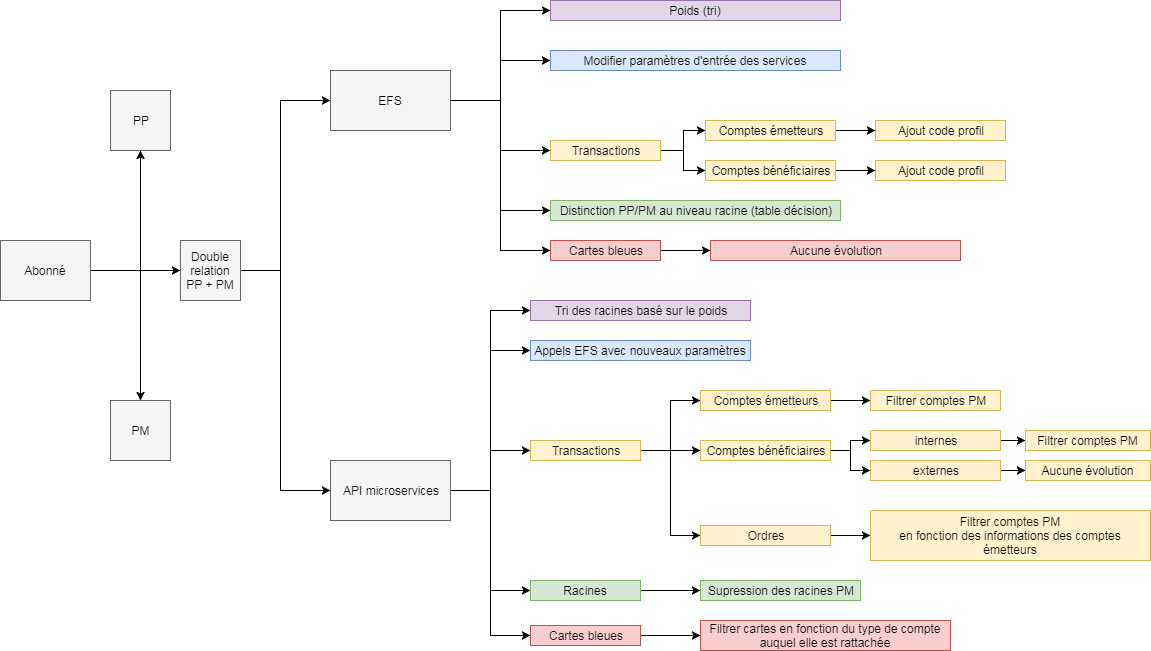
\includegraphics[scale=0.45]{images/travailNeuflizeOBC/doubleRelation/doubleRelation.png}
	\centering
	\caption{Objets impactés par les doubles relations}
	\label{doubleRelation}
\end{figure}

	Il était maintenant possible de déterminer les services qui aurraient besoin de développement supplémentaire. D'après ce schéma, les services concernés étaient ceux présent dans le tableau figure \ref{servicesDoubleRelation}. Une fois cela établi il ne restait plus qu'à procéder au développement et à effectuer les modifications nécessaires afin d'assurer la gestion des doubles relations dans la couche API microservices. \\ 
	
\begin{table}[h!]
	\center
	\begin{tabular}{| c | c | c |}
     \hline
     Service & Raison \\ \hline
     accountToDebit & Créer un filtre sur les comptes émetteurs \\ \hline
     addressBook & Créer un filtre sur les comptes bénéficiaires internes \\ \hline
     transactionOverview & Créer un filtre sur les ordres de transaction\\ \hline
     clientList & Créer un filtre sur les racines récupérées \\ & et les trier selon leur poids\\ \hline
     accountOverview & Créer un filtre sur les cartes bleues \\
     Tous & Rajouter le paramètre "codeProfil=PP" dans les appels aux services EFS \\ 
     \hline
	\end{tabular}
	\caption{Modifications par services pour la gestion des doubles relations}
	\label{servicesDoubleRelation}
\end{table}

\subsection{Résultats}

	Comme nous l'avons vu, les modifications à apporter sont mineures et les nouveaux développements sont loin d'être conséquents, mais ces derniers impactent de très nombreux endroits du code et nécessite d'altérer plusieurs services ce qui aurraient pu gêner les autres développeurs dans leur travail. De plus, EFS n'étant pas prêt de son côté, j'ai travaillé en utilisant \textit{WireMock}, un outil permettant de créer des \textit{mocks} qui sont des objets simulés reproduisant le comportement d'objets réels. Ainsi, cela m'a conforté dans l'idée de créer une nouvelle branche sur le github du projet sur laquelle j'ai poussé le code permettant la gestion des doubles relations. Une fois EFS prêt, il sera alors facile de simplement réaliser un merge de cette branche avec la branche master. \\
	
	Bien que la réalisation de cette tâche ne présentait pas de grandes difficultés d'un point de vue de technique, celle-ci m'a permis de me familiariser avec l'aspect relationnel du projet. En effet, nous travaillons en employant des méthodes agiles ce qui m'a conduit a rencontrer le client c'est-à-dire les métiers travaillant dans le même openspace que nous. Ceci m'a permis d'avoir une première expérience complète, bien qu'à petite échelle, allant de la définition du besoin avec le client jusqu'à la réalisation de la fonctionnalité en accompagnant celui-ci tout au long du processus via diverses réunions afin de fixer les points cruciaux. Ensuite, j'ai pu réaliser cette tâche de manière autonome et donc eu la chance de pouvoir mettre en place mes propres solutions tout comme pour la partie concernant les tests fonctionnels, à ceci prêt que dans ce cas il ne s'agissait pas d'un travail indépendant mais en relation direct avec le code source et une livraison, impliquant une certaine confiance.
	En outre, j'ai été contraint d'apporter des modifications à travers toute l'API ce qui m'a permis de pouvoir mieux m'approprier le code et de monter ainsi en compétence sur la stack utilisée et surtout sur le développement de "microservices".
	
\section{Dashboard}
	\subsection{Cachier des charges}
		La mise en production de l'application mobile approchant, le client a émis le souhait de pouvoir collecter des données sur la manière dont les utilisateurs l'utiliseraient. Il souhaitait avoir à sa disposition un outil lui permettant de monitorer l'application afin de pouvoir évaluer la satisfaction des utilisateurs et de relever les axes d'amélioration. 
	
	Par exemple, pour réaliser une transaction bancaire via l'application mobile, l'utilisateur doit se connecter puis initier la transaction en choisissant des comptes émetteurs/receveurs ainsi qu'un montant. Après cela, un clavier virtuel apparait sur lequel il doit rentrer son code secret, ce qui aura pour effet de \textit{signer} la transaction. Une des requêtes de Neuflize était de pouvoir avoir un ratio entre le nombre de transaction initiée et le nombre de transaction signée afin de déterminer les nombres de transaction abandonnée en cours de création et donc si ce système de signature ne rebutait pas les utilisateurs dans leur démarche. En effet, un grand nombre de transaction initiée mais non signée pourrait indiquer que cette procédure ne plait pas aux clients de la banque parce qu'elle serait trop longue ou peu pratique. De plus, cela permettrait aussi de suivre les potentielles erreurs qui apparaitraient entre l'initiation et la signature afin de prendre des mesures adéquates. \\
	
	Afin de suivre ces informations, Neuflize souhaitait pouvoir disposer d'un \textit{dashboard} (tableau de bord), qui centraliserait l'ensemble des données collectées sous la forme de graphiques. Le dashboard contiendrait alors tous les graphiques et permettrait de naviguer facilement afin de retrouver les informations recherchées, et ce en fonction du temps. En effet, le critère de temps est indispensable dans l'optique de suivre l'évolution de l'applicaton et pour situer les événements.
	
	Ainsi, avant que la réalisation d'un tel dashboard me soit confiée, les outils qui seraient utilisés avaient été décidé suite à une réunion entre l'un des architectes du projet et les métiers. Il m'a donc été demandé de répondre à ce besoin en mettant en place, dans un premier temps, la stack ELK (Elasticsearch, Logstash et Kibana) dont nous parlerons dans la partie suivante puis en créant une première ébauche des graphiques en local à l'aide de données factices. En outre, une deadline avait été fixée puisque le dashboard, ou du moins la collecte des données, devait être prêt pour la mise en production de l'application. En effet, les premières informations sont essentielles pour déterminer les évolution à apporter à l'application et permettent d'avoir une idée de la satisfaction des utilisateurs. \\
	
	Il m'a été remis un document réalisé par Neuflize, dont un extrait est disponible figure \ref{elkBesoin}, dans lequel il était décrit l'ensemble des besoins c'est-à-dire toutes les informations qui étaient souhaitées, comment elles devaient être traitées et la manière dont elles devaient être gérées. Le premier travail à effectuer a été de déterminer quelles informations pouvaient être remontées par l'API microservices et lesquelles ne le pouvaient pas. Par exemple, nous pouvons voir qu'il était demandé le nombre de transaction initiée sur une période donnée, chiffre qu'il est possible pour nous de fournir. Cependant, il est aussi demandé le temps passé sur chaque écran de l'application par l'utilisateur ou encore le nombre de page que celui-ci a visité, ce qui est impossible à fournir de notre côté. En effet, la couche API microservices est bien évidemment situé dans la partie backend du projet et est une API REST exposant des services. Ainsi, il nous est totalement impossible d'obtenir des informations si nos services ne sont pas appelés. Le temps passé sur chaque écran n'est pas calculable puisque certains écrans peuvent ne pas appeler de services, certains en appeleront plusieurs etc... Il a donc fallu analyser l'ensemble des besoins dans le but de déterminer ce qui était réalisable de notre côté, quant au reste, il était possible de l'obtenir du côté frontend via d'autres outils qui avaient été mis en place par l'équipe en charge de cette partie tel qu'\textit{Omniture}.
	
\begin{figure}[h!]
	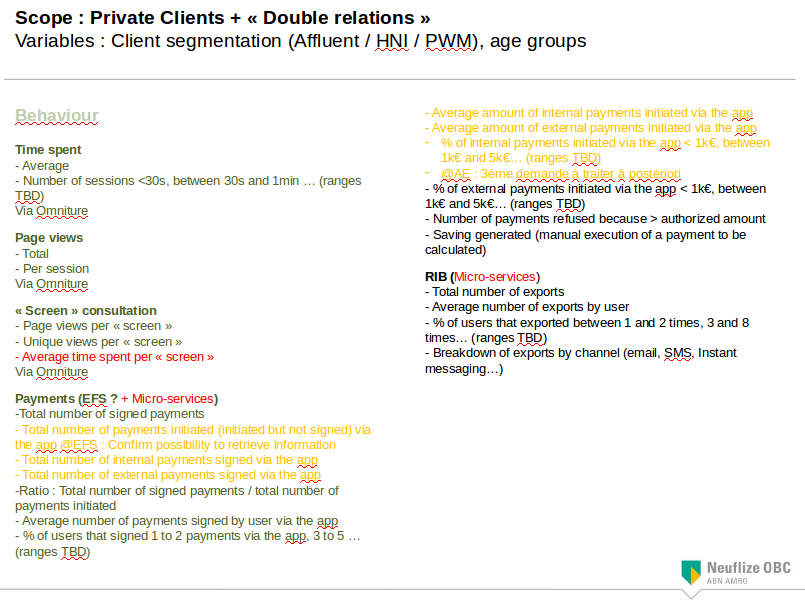
\includegraphics[scale=0.6]{images/travailNeuflizeOBC/dashboard/elkBesoin.png}
	\centering
	\caption{Extrait du besoin client pour le dashboard}
	\label{elkBesoin}
\end{figure}
	
	Une fois cette étude terminée j'ai effectué un rapport auprès d'un architecte du projet qui a validé mon analyse puis j'ai organisé une réunion avec les métiers afin de clarifier la situation et leur faire savoir tout ce qui était faisable par l'API microservices. Au terme de cette réunion et après discussion sur la manière de remplacer certaines informations inaccessibles par d'autres s'en rapprochant ou permettant de les retrouver, j'ai pu me lancer dans la mise en place de la stack ELK et la réalisation du premier jet du dashboard.

\subsection{La stack ELK : ElasticSearch, Logstash et Kibana}
		Comme nous l'avons dit précédemment, pour réaliser le dashboard il a été décidé que la stack ELK serait utilisée. J'ai donc, dans un premier temps, du me former à l'utilisation de cette dernière qui est constituée de trois produits de la société Elastic que sont Elasticsearch, Logstash et Kibana. Son objectif premier est de stocker, d'analyse et de lire les logs générer par un projet tel qu'une API REST dans l'optique de faire du monitoring, de suivre l'activité d'un service ou de prévenir des dysfonctionnements. Nous allons maintenant décrire en quoi chacun des outils est intervenu dans le processus de réalisation du dashboard. Pour cela, il est possible de se référer à la figure \ref{elk} afin de pouvoir situer chaque composant.

	\subsubsection{Elasticsearch}
	La quantité de logs générés par une application de cette ampleur peut rapidement devenir très conséquente et de nombreuses problématiques sont alors soulevées concernant le stockages des messages importants, leur recherche ou leur analyse. Les bases données relationnelles classiques ont montré leurs limites concernant le travail avec de tels volumes de données sur le long terme que ce soit pour le stockage ou les temps de réponse lors d'une recherche, et ce malgré des requêtes bien construites avec des jointures judicieuses entre les tables. Elasticsearch a pour objectif de répondre à cette problématique. \\
	
	Il s'agit d'un moteur d'indexation, de stockage et de recherche de données développé en Java basé sur \textit{Lucene}, une bibliothèque d'indexation et de recherche de texte créée par la fondation Apache. Son principal atout est qu'il permet de stocker de large volume de données tout en permettant aux utilisateurs d'effectuer des recherches en temps réel. Les données sont stockées sous la forme de \textit{document}. Il s'agit d'une unité basique d'information qui peut être indexée. Les index sont des collections de documents possédant des caractéristiques similaires. Les index peuvent aussi posséder un type afin de les diviser en plusieurs parties "logiques". On peut, par exemple, créer un index \textit{api-microservices-2017.07} avec un type \textit{log}. 
	
	On pourra alors récupérer le document d'id 1 avec la requête suivante :	

\begin{lstlisting}[language=json]
 GET api-microservices-2017.07/log/1?pretty
 \end{lstlisting}
	
	La réponse contiendrait ledit document avec les champs définis par nos soins (ici timestamp, logLevel, service et message) :
	
\begin{lstlisting}[language=json]
{
 "_index": "api-microservices-2017.07",
 "_type": "log",
 "_id": "1",
 "_version": 1,
 "found": true,
 "_source" : {
  "timestamp": "2017-07-07T14:15:45",
  "logLevel": "INFO",
  "service": "account-service"
  "message": "elasticsearch example"
 }
}
	\end{lstlisting}
	 
	 Dans notre cas, Elasticsearch est utilisé comme support de stockage qui sera par la suite interrogé par Kibana. Cependant, il peut tout à fait être interroger depuis une API, c'est pourquoi il ne dispose pas de client dédié.
	
	\subsubsection{Logstash}
	Logstash est un \textit{ETL} ou \textit{Extract-transform-load}. Cela désigne les outils capable de synchroniser des volumes de données massif depuis une source précise vers une autre. Ainsi, Logstash agit un peu à la manière d'un pipeline capable de prendre un grand nombre de messages en entrée depuis plusieurs sources pour les traiter, effectuer des transformations ou encore les filtrer avant de les renvoyer vers un support de stockage. Le schéma figure \ref{logstash} explicite son principe de fonctionnement. La liste des technologies mentionnées dans celui-ci n'est pas exhaustive, il s'agit purement d'exemples de ce qu'il est possible de faire à titre démonstratif. \\
	
	\begin{figure}[h!]
		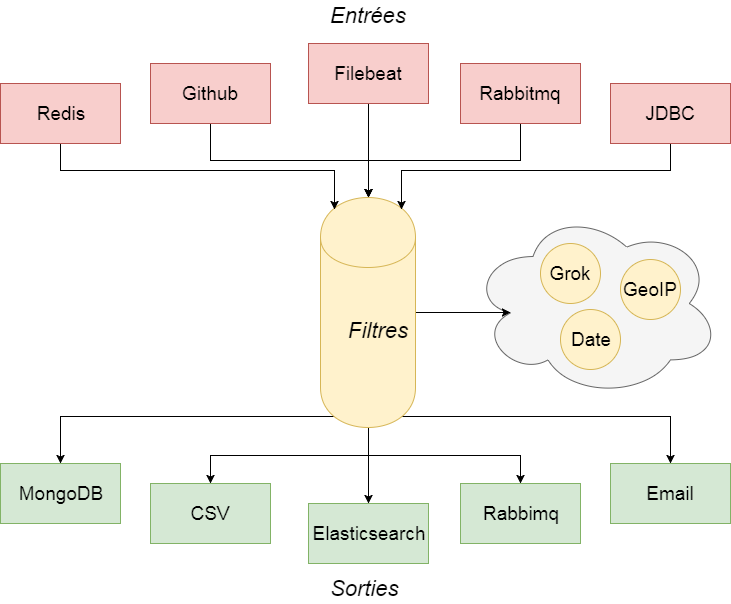
\includegraphics[scale=0.4]{images/travailNeuflizeOBC/dashboard/logstash.png}
		\centering
		\caption{Logstash}
		\label{logstash}
	\end{figure}
	
	Logstash accepte en entrée un nombre impressionnant de formats différents comme tout ce qui est représenté sous forme de chaîne de caractères mais aussi les événements issus de sources différentes et ce de manière simultanée. Dans notre cas, logstash prendra en entrée des fichiers logs fournit par Filebeat dont nous parlerons plus en détails peu après. Ces logs auront été générés au préalable par l'API microservices à l'aide de \textit{Logback}. \\
	
	Une fois les données acquises, celles-ci sont analysées puis transformer par les filtres de Logstash. Il est ainsi possible d'ajouter, modifier ou supprimer de l'information, extraire des valeurs depuis des messages, analyser des événement et bien d'autres. Le filtre le plus puissant mis a disposition par Logstash est \textit{Grok} que nous utiliserons ici et qui permet de transformer dynamiquement des données non structurées en données structurées en découpant une ligne de log en un ensemble de champs prédéfinis. Nous pourrons donc utiliser ce filtre afin de structurer les informations de telle manière qu'elles soient facilement exploitable par Kibana. Par exemple, la ligne de log suivante :
	
\begin{lstlisting}[language=json]
 [2017-07-07T14:15:45] [INFO] [account-service] - elasticsearch example
\end{lstlisting}
	
	peut être transformer sous la forme du document structuré montré en exemple plus haut à l'aide d'un filtre adéquat définissant les champs (comme timestamp ou loglevel). \\
	
	Enfin, une fois les données formatées, il est possible de les envoyer vers la destinaiton de notre choix, et là encore Logstash offre la possibilité de transmettre les données vers un grand nombre de sources différentes. Il sera bien évidemment ici connecté à Elasticsearch et permettra donc de stocker les logs de manière structurée et indexée au sein de la base de données. En outre, il offre une grande flexibilité puisque chacune des entrées/sorties ou mêmes les filtres sont implémentés sous la forme de plugin. Par ailleurs, la société Elastic a mis à disposition une API permettant de faciliter le développement de ces plugins, ce qui permet d'ajouter de nombreuses nouvelles possibilités à Logstash.
	
	\subsubsection{Kibana}
	Avec les outils précédent nous avons de quoi stocker nos logs, les analyser, les transformer pour structurer les informations qu'ils contiennent et rechercher ce que nous souhaitons parmis eux à l'aide de requêtes Elasticsearch. Cependant, cela n'est absolument pas "user friendly" et nécessite des connaissances techniques ce qui ne suffit pas à satisfaire le besoin client. Kibana permet palier cette faiblesse en nous fournissant une interface nous permettant de choisir la mise en forme de nos données. Celui-ci permet de construire des graphiques, nommés \textit{visualisations}, tels que des histogrammes, des camemberts ou encore des tableaux. Ensuite, Kibana permet de choisir une plage de date pour ne traiter que les données situées dans cette dernière. Une fois le dashboard et les visualisations créés, il suffit de changer le temps et tous les graphiques s'actualiseront automatiquement ce qui permet de facilement retrouver des informations. Par exemple, il suffit d'un simple clic pour connaitre le nombre de connexion qu'il y a eu hier, le mois dernier ou entre le 23 juillet et le 15 août. De plus, Kibana vient avec une nouvelle composante nommée \textit{Timelion} permettant d'effectuer des analyses chronologiques approfondies. \\
	
	Ici, Kibana alimentera les visualisations avec les données stockées dans la base d'Elasticsearch et sera l'unique interface homme machine utilisée. En effet, il offre une console développeur permettant de faciliter la construction des requêtes Elasticsearch et permet de visualiser les données stockées en base à l'aide une option \textit{discovery} affichant pour chaque ligne de log brute les champs structurés définis dans logstash.
	
	\subsubsection{Filebeat}	
	Elastic a mis à notre disposition, en plus de la stack ELK, des agents de transfert nommés les \textit{Beats}. Il en existe pour tout type de données mais dans notre cas nous utiliserons Filebeat conçu spécialement pour le transfert des logs et fichiers. Celui-ci permet de collecter l'ensemble des logs, qu'importe où ils se trouvent, pour les envoyer ensuite à Logstash. Il est possible de le configurer pour qu'il ne transfert pas les fichiers de logs entiers mais seulement les lignes qui nous intéressent. Celui-ci ne nécessite aucune intervention humaine une fois qu'il est mis en place, à chaque ligne de log générée il en est informé et effectue le transfert automatiquement. En outre, si Logstash est occupé et possède déjà un gros volume de données à traiter, Filebeat en sera également informé et pourra ralentir son flux d'envoi afin d'éviter tout problème de congestion.

	\subsubsection{Les intéractions en résumé}
	Toutes les intéractions entre les différents composants sont résumées sur le schéma figure \ref{elk}. Pour commencer, les logs sont générés par l'API microservices grâce à Logback qui permet de configurer quelle ligne ira dans quel fichier et où ces derniers seront créés. Dès que des lignes de logs sont générées, Filebeat est averti et va donc lire le fichier de logs concerné, détecter les nouvelles lignes puis les envoie à Logstash si elles remplissent les critères. Ce dernier récupère ces lignes non structurées en entrée et agit comme un pipeline qui produira en sortie des données structurés à l'aide de champs prédéfinis. Ensuite, Elasticsearch reçoit ces données de la part de Logstash, les indexe puis les stocke en base de données. Enfin, Kibana interroge Elasticsearch à l'aide de requêtes en fonction du temps sélectionné pour alimenter les visualisations créées au sein du dashboard. 
	
\begin{figure}[h!]
	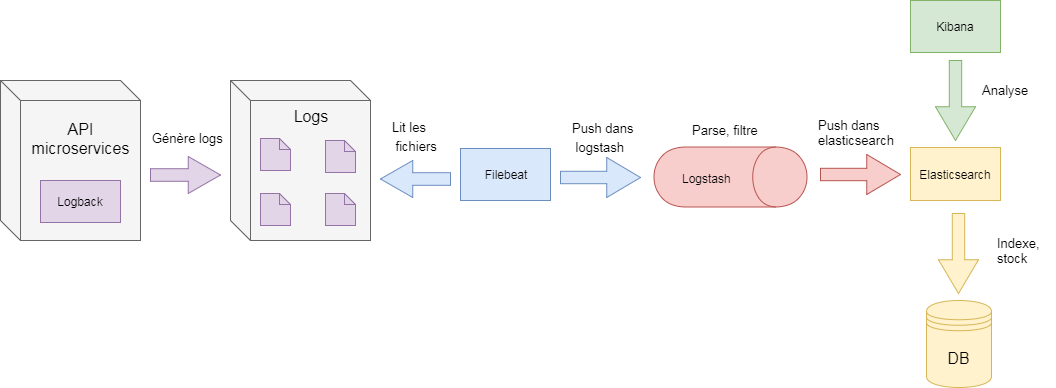
\includegraphics[scale=0.5]{images/travailNeuflizeOBC/dashboard/elk.png}
	\centering
	\caption{Intéractions au sein de la stack ELK}
	\label{elk}
\end{figure}
	
\subsection{Réalisation des graphes}
		Comme nous l'avons vu dans la partie précedente, les données qui seront exploitées sont des logs. Ainsi, après avoir installé et configuré les différents éléments de la stack ELK, mon objectif était de générer des logs afin que puisse tester chacune des composantes entrant en jeu. Cependant, avant d'aller plus loin, il faut savoir que l'API microservices génère déjà de nombreux logs informatifs permettant d'analyser les actions effectuées, l'état des services ou encore les erreurs. De plus, il existe d'autres outils comme RabbitMQ, un message broker, qui génère une grande quantité de logs. Les lignes qui nous intéressent pour construire les visualisations sont donc noyées dans un flot d'information qui ne cesse de croître à mesure que le temps s'écoule. La première étape a donc été de définir un modèle permettant de différencier les lignes de logs qui seraient destinées au dashboard de celles qui ne le sont pas. \\
	
	\subsubsection{Mise en place du modèle}
	
	Grâce à Logback, tous les logs de l'API suivaient le même pattern constitué d'une première partie auto-générée et d'une seconde partie contenant le message effectivement loggé. Par exemple, dans le code la ligne suivante :

\begin{lstlisting}[language=json]
 LOGGER.info("message");
\end{lstlisting}	

 aurait pour effet de générer la ligne de log suivante :

\begin{lstlisting}[language=json]
 [timestamp] [host] [thread] logLevel class@method:line - message
\end{lstlisting}

avec :

\begin{table}[h!]
	\center
	\begin{tabular}{| c | c |}
     \hline
     timestamp & Date d'émission du log \\ \hline
     host & VM sur laquelle le log a été émis \\ \hline
     thread & Thread depuis lequel le log a été émis \\ \hline
     loglevel & Niveau du log (INFO, WARNING, ERROR etc...) \\ \hline
     class & Classe depuis laquelle le log a été émis \\ \hline
     method & Méthode depuis laquelle le log a été émis \\ \hline
     line & Ligne à laquelle le log a été émis \\ \hline
     message & Le contenu du log \\
     \hline
	\end{tabular}
	\caption{Log - première partie}
	\end{table}
	
	J'ai décidé que les logs à destination de Kibana contiendraient un message commençant par le mot-clé \textit{ANALYTICS}. Ainsi, j'ai configuré FileBeat pour qu'il n'envoie que les logs dont le message commençait par ce mot à Logstash et qu'il ignore les autres. La suite du message contiendrait toutes les informations nécessaires pour élaborer les graphiques. Parmi ces informations, les suivantes seraient obligatoires et entourées de crochet :
	
	\begin{table}[h!]
	\center
	\begin{tabular}{| c | c |}
     \hline
     username & Login de l'abonné envoyant les requêtes \\ \hline
     microservice & Microservice depuis lequel le log a été émis \\ \hline
     service & Service depuis lequel le log a été émis \\
     \hline
	\end{tabular}
	\caption{Log - deuxième partie}
	\end{table}
	
	Une ligne finale ressemblerait donc a :
	
\begin{lstlisting}[language=json]
 [timestamp] [host] [application] logLevel class@method:line - [ANALYTICS] [username] [microservice] [service] info1=valeur1 info2=valeur2 ... infoN=valeurN 
\end{lstlisting}
	
	J'ai ensuite placé la génération de log dans tous les services de l'API. Pour le service NewTransfer permettant d'initialiser une transaction bancaire nous pouvions par exemple obtenir :
	
\begin{lstlisting}[language=json]
[2016-06-26 08:11:34.086] [FR7WSPAR54464] [main] INFO c.n.a.m.t.logstash.LogStashTests@testNewTransfer:36 - [ANALYTICS] [COCKZAO72] [Transaction] [NewTransfer] transactionId=13072409724 totalAmount=1000 paymentMode=SINGLE currency=EUR internal=true
\end{lstlisting}

	Les informations optionnels transactionId, totalAmount, paymentMode, currency et internal sont propres au service NewTransfer et ne seront pas présentes dans les logs des autres services. 
	
	\subsubsection{Configuration de Logstash}
	
	Tous ces logs seront envoyé par Filebeat à Logstash qui aura pour objectif de les structurer à l'aide de filtres. Il est possible de définir plusieurs filtres qui seront alors appliquer dans l'ordre les uns après les autres. Ainsi, j'ai créé un premier filtre permettant de parser la première partie des logs depuis le timestamp jusqu'au nom du service. Cette partie étant commune à tous les logs, ce filtre est toujours appliqué et en premier. Celui-ci se présente sous cette forme :
	
\begin{lstlisting}[language=json]
filter {
 grok {
  match => {
   "message" => "(?m)\[%{TIMESTAMP_ISO8601:timestamp}\] \[%{HOSTNAME:host}\] \[%{DATA:thread}\] %{LOGLEVEL:logLevel} %{DATA:class}@%{DATA:method}:%{DATA:line} \- \[ANALYTICS\] \[%{DATA:username}\] \[%{DATA:microservice}\] \[%{DATA:service}\]"
  }
 }

 date {
  match => ["timestamp" , "YYYY-MM-dd HH:mm:ss.SSS"]
  target => "@timestamp"
 }
}
\end{lstlisting}

	Nous pouvons observer la présence d'un filtre Grok avec une instruction \textit{match}. Si ce filtre est placé en premier, il récupère la ligne de log et essaie de la faire matcher avec le pattern défini dans l'instruction match. Les chaînes en majuscule désigne des constantes représentant les types de données supportés par Logstash. Par exemple, la première valeur entre crochet du log sera stockée dans le champ timestamp et sera de type TIMESTAMP\_ISO8601 alors que la dernière sera stockée dans le champ service et sera de type DATA (c'est-à-dire tout type de caractères). Une fois tous les champs créés, un second filtre \textit{date} permet de parser le timestamp précédemment recueilli pour l'utiliser comme date pour l'événement logstash. Kibana se basera par la suite sur cette date pour construire les visualisations. \\
	
	Si nous reprennons notre exemple de log avec NewTransfer, nous pouvons nous apercevoir ici que les informations optionnels ne sont pas encore matchées. Pour ça il faut rajouter un second filtre qui s'en chargera. De manière générale, j'ai créé de nombreux filtres pour chacun des services de l'API. Pour chacun de ceux-là j'ai placé une condition afin qu'ils ne soient appliqués que pour le service correspondant. Ainsi, dans notre exemple, le champ service prend la valeur "NewTransfer" et donc seuls les filtres NewTransfer seront par la suite appliqués. \\
	
	Une fois tous les filtres exécutés, les données sont structurées et sont envoyées à ElasticSearch qui se charge de les indexer sous la forme de document puis de les stocker en base. Il est possible de préciser, juste après les filtres, l'index qui sera utilisé. Ici j'ai choisi : \textit{api-microservices-YYYY.MM} (où YYYY.MM désigne la date). De ce fait, un index sera créé tous les mois afin de faciliter la recherche des informations sur Kibana. 
	
	\subsubsection{Création des visualisations sur Kibana}
	
	A ce stade, la configuration Logstash est terminée et nos logs sont bien envoyés à ElasticSearch. La dernière étape est donc de créer les différents graphiques exploitant nos données sur Kibana. Le client a seulement spécifié les données qu'il souhaitait pouvoir consulter et non la forme sous laquelle elles devaient apparaître c'est pourquoi j'ai à chaque fois essayé de choisir des graphiques adaptés parmi les types qui existaient (table, camembert etc...). Kibana vient avec une interface web sur laquelle il est possible de choisir une visualisation puis d'y associer une requête ElasticSearch afin de l'alimenter. Afin de pouvoir avoir un aperçu des graphiques rapidement j'ai créé des tests unitaires qui ne faisaient que générer des logs. Ensuite, il était possible d'exécuter ces tests via Spring pour générer autant de logs que j'en avais besoin pour construire mes visualisations sans avoir a réellement envoyer des requêtes vers l'API. \\
	
	Lors de la création d'une visualisation, Kibana met à notre disposition des outils permettant de choisir, par exemple, quel type d'opération nous souhaitons effectuer sur les données : les compter, prendre le maximum, les additionner etc... ou encore quel type d'agrégation nous voulons mettre en place. Cela permet de construire les requêtes ElasticSearch qui fourniront les données à afficher. Toujours sur l'exemple de NewTransfer, l'un des besoins était de pouvoir suivre le montant des virements effectués via l'application mobile. Pour cela, j'ai décidé de faire un diagramme de type \textit{donut} dont plusieurs exemples sont disponibles en annexe \ref{c1}. Ce diagramme est construit sur la requête suivante :
	
\begin{lstlisting}[language=json]
{
 "size": 0,
 "query": {
  "match": {
   "service": "NewTransfer"
  }
 },
 "aggs": {
  "aggMontant": {
   "range": {
    "field": "montant",
	"ranges": [{
	 "from": 0,
	 "to": 200
	},
	{
	 "from": 200,
	 "to": 400
	},
	{
	 "to": 600,
	 "from": 400
	},
	{
	 "to": 800,
	 "from": 600
	},
	{
	 "to": 1000,
	 "from": 800
	},
	{
	 "from": 1000
	}
	],
	 "keyed": true
   }
  }
 }
}	
\end{lstlisting}

	Nous commençons par préciser que l'on ne match que les documents dont le champ \textit{service} a pour valeur "NewTransfer". Ensuite, nous réalisons une \textit{agrégation} sur les données récupérées. Les agrégations sont des opérations permettant de résumer les données de manière complexe. Ici, elle est de type \textit{range} et a pour but de classer les données selon des intervalles de valeur défini en dessous. Nous précisons ici que le classement s'effectuera sur la valeur du champ montant. \\
	
	Malheureusement, j'ai rencontré quelques problèmes durant la création des visualisations. En effet, il s'est avéré que certains besoins ne pouvaient finalement pas être satisfaits. Par exemple, les métiers souhaitaient pouvoir suivre le nombre d'abonnés qui s'étaient connectés à l'application et trier cela sur des intervalles (10 abonnés se sont connectés entre 0 et 50 fois, 15 abonnées entre 50 et 100 fois etc...). Si j'ai finalement pu réussir à construire une requête ElasticSearch pour obtenir de telles données, il n'y avait aucune visualisation Kibana qui pouvait l'accueillir ou la reconstituer. Pour pallier cela j'ai essayé de fournir d'autres visualisations répondant à un besoin se rapprochant le plus possible de celui d'origine afin que le client puisse quand même accéder à certaines données même si cela était moins pratique.
	
	Je pense que la principale erreur était que si la stack ELK permet de effectivement de faire du monitoring, elle n'est pas faite pour du monitoring métier mais plutôt pour du monitoring technique. Par exemple, surveiller les temps de réponses, les erreurs au sein des services, observer les performances etc... De plus, je pense aussi que j'aurais du aller un peu plus en profondeur dans mon étude de Kibana avant d'organiser la réunion avec le client au cours de laquelle nous avons défini les besoins qui seraient satisfait. J'ai découvert par la suite que Kibana propose une option avancée sur ses visualisations avec laquelle il est possible de passer des paramètres en JSON qui seront par la suite mergé avec l'agrégation qu'il réalise. Cependant, je n'ai pas pu approfondir cette possibilité faute de temps et de documentation à son sujet. \\
	
	En outre, depuis la création du dashboard, de nouvelles versions de Kibana sont sorties, apportant de nouvelles visualisations ainsi que de nouveaux outils plus performant pour construire les graphiques. Il pourrait être intéressant de vérifier si certains besoins pourraient maintenant être comblés et, le cas échéant, mettre Kibana à jour. Une autre solution, bien que peu envisageable maintenant, aurait pu être d'utiliser un autre outil que Kibana, compatible avec ElasticSearch comme par exemple Grafana.
	
\subsection{Dashboard final}
		Le dashboard étant maintenant terminé, une phase de recette a été organisée avec deux métiers ainsi que mon chef de projet afin que je puisse présenter le travail que j'avais effectué. Tous les graphiques ont été passés en revue et les métiers ont pu vérifier que chacun des besoins que je m'étais engagé à satisfaire était effectivement présent sur ledit dashboard.

\begin{figure}[h!]
	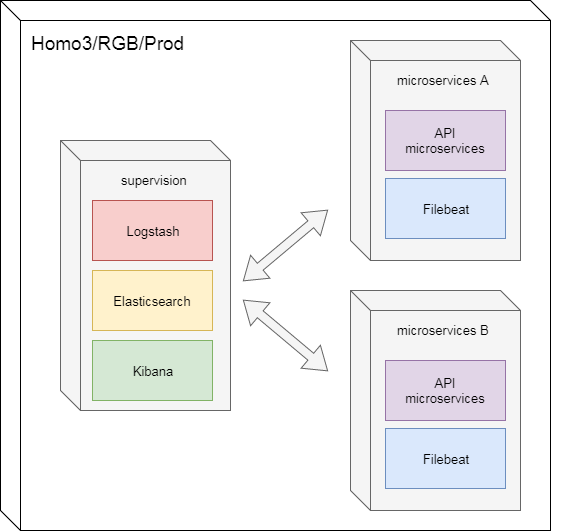
\includegraphics[scale=0.5]{images/travailNeuflizeOBC/dashboard/elkDeploiement.png}
	\centering
	\caption{Architecture de la stack ELK sur tous les environnements}
	\label{elkDeploiement}
\end{figure}
%-----------------------------------------------------------------------------------------------------------------
%-----------------------------------------------------------------------------------------------------------------
	
%-----------------------------------------------------------------------------------------------------------------
%-----------------------------------------------------------------------------------------------------------------

\chapter{BP1818}

	\fancyhead[LE]{
	\begin{picture}(0,0) 
	\put(-30,-5){
\includegraphics[width=37mm]{images/bp1818Logo.png}}
	\end{picture}
}
\fancyhead[LO]{
	\begin{picture}(0,0) 
	\put(-8,-5){
\includegraphics[width=37mm]{images/bp1818Logo.png}}
	\end{picture}
}

\section{Présentation du projet}
	\begin{itemize}
	\item Trois canaux : banquier/selection/cgpi
	\item Entrée en relation, ouverture de comptes titres, souscription AV
	\item La MIF
	\item Méthodes agile (sprint, sprint planning, scrum poker, sprint review, TU, qualif, ateliers)
	\item Daily meeting
\end{itemize}

\section{Architecture logicielle de l'application}
	\paragraph{}
Dans cette partie nous allons présenter plus en détails l'architecture globale du projet d'application mobile de Neuflize OBC. Comme nous l'avons vu précédemment, ce projet est basé sur une architecture multicouches dont la structure est représentée dans sa globalité en annexe \ref{a2}. Nous allons maintenant décrire chacune des couches afin de comprendre le fonctionnement du projet. Cependant, les technologies employées étant nombreuses, il serait peu pertinent de toutes les expliciter, ainsi seul l'essentiel en lien avec le stage sera ici décrit. Toutefois, il est possible de retrouver toutes les briques en annexe.

\subsection{Axway API Gateway}
\label{axway}

	Deux instances de l'API Gateway d'Axway ont été installées en mode « actif/actif » afin d'assurer la mise en place de la couche \textit{security} et celle de la couche \textit{management}. La répartition de charge est gérée par l'instance positionnée en amont. \\
		
	L'API Gateway de la couche security est le serveur traitant les appels API. Cette dernière est en charge de la sécurité applicative des appels vers la couche API Management. Elle est positionnée dans le tier 1, reçoit les appels « HTTPS » et a principalement pour objectif d’effectuer les actions suivantes : \\
	
	\begin{itemize}
		\item Vérifier la validité des certificats partenaires
		\item Filtrer les requêtes entrantes 
		\item Agir comme un pare-feu applicatif afin de vérifier le contenu des messages REST
		\item Répartir la charge vers les composants en aval
		\item Protéger le SI en limitant le nombre d’appels API via un mécanisme de régulation du traffic et en limitant le nombre d'appels au SI via un mécanisme de cache \\
	\end{itemize}
	
	La couche API management, dans le tier 2, permet de configurer et d’exposer les API. Elle assure les fonctionnalités suivantes : \\
	
	\begin{itemize}
		\item Publier et sécuriser les API
		\item Gérer le cycle de vie des API
		\item Gérer l’authentification et les habilitations (développeurs et administrateurs API)
		\item Embarquer les développeurs d’applications consommatrices d’API
		\item Auditer, suivre la consommation des API, gérer les quotas
		\item Assurer la haute disponibilité \\
	\end{itemize}
	
	Une interface web avait aussi été mise à notre disposition par Axway, nous permettant de traquer toutes les requêtes effectuées. \\
	
	Afin d'assurer la sécurité l'API management utilise \textit{OAuth2} ainsi que \textit{JWT}. OAuth2 est un framework d'authentification permettant d'authentifier plusieurs applications différentes. JWT est un protocole d'authentification permettant de créer et valider des \textit{tokens} (ou jetons) de sécurité. Ces tokens sont ensuite utilisés pour limiter l'accès des utilisateurs aux API. Pour chaque utilisateur qui se connecte, la Rest Layer envoie une assertion SAML. Si cette assertion est vérifiée par l'API management un token est généré contenant les informations permettant à un utilisateur d'accéder aux ressources protégées. Ainsi, toute les requêtes émises vers l'api microservices doivent contenir un token permettant l'authentification sans quoi elles seront rejetées (erreur 401 : Unauthorized). J'ai simplifié ici la procédure et limité les informations à ce qui est nécessaire pour la compréhension du rapport. En effet, celle-ci est extrêmement complexe et dépasse ce qui a été effectué dans le cadre du stage.
	
\subsection{Microservices}

	Avant d'aller plus loin, nous allons expliciter ce qu'est une architecture microservices \cite{bib_microservices} afin de pouvoir comprendre la structure des API. Il s'agit d'un paradigme d'architecture qui jouit actuellement d'une grande popularité aux dépends de celles plus classiques (N-tiers, SOA...), inventée afin de répondre aux problématiques soulevées par les projets de grande ampleur. \\
	
	Cette approche consiste à développer une application sous forme d'un ensemble de services dont la granularité correspond à une fonctionnalité élémentaire en terme métier. Chacun de ces services doit posséder son propre contexte d'exécution et ainsi être testable et déployable indépendemment en favorisant un couplage le plus faible possible. Ils peuvent être écrit dans des langages différents et communiquer entre eux via, par exemple, le protocole HTTP et la mise en place d'une API REST, ce qui est le cas pour ce projet. On parle alors de microservices, terme qui s'oppose aux applications plus classique que l'on dit monolithiques.\\
	
	Les applications d'entreprises classiques sont très souvent construites sur une architecture trois tiers constituées de trois parties majeures :
	\begin{itemize}
		\item Une interface client permettant la présentation des données
		\item Un serveur contenant la logique métier et effectuant le traitements des données
		\item Une couche d'accès aux données permettant de gérer les données persistantes \\
	\end{itemize}
	
\begin{figure}[h!]
	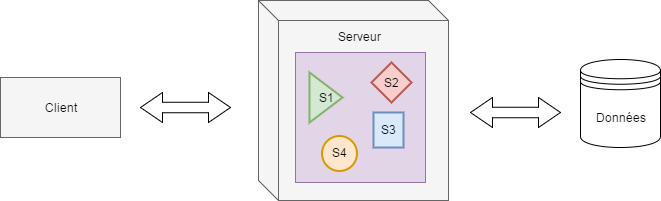
\includegraphics[scale=0.5]{images/travailNeuflizeOBC/architecture/troisTiers.png}
	\centering
	\caption{Architecture trois tiers monolithique}
	\label{troisTiers}
\end{figure}
	
	L'ensemble des services est contenu dans la même application et ces derniers sont donc exécutés dans un même processus. Ainsi, le moindre changement nécessite de rebuild et redéployer l'application entièrement. La scalabilité horizontale (par exemple un ajout de serveur) en est impactée. En effet, l'application entière doit être migrée si l'on souhaite changer de matériels afin d'améliorer les performances. Si un certain module est plus lent, il n'est pas possible de le déplacer indépendemment afin d'améliorer son exécution, il faut répliquer le monolithe entier tandis que du côté des microservices il est possible de répliquer un service en particulier et d'en redéployer un sans avoir à redéployer tout l'ensemble. De plus, dans les gros projets, la quantité de code a tendance à augmenter rapidement impliquant une hausse de la compléxité et rendant ainsi difficile l'ajout de nouvelles fonctionnalités. Le couplage entre ces dernières devient fort et les nombreux effets de bords résultant de chaque modifications rendent alors l'application moins fiable, limitant les perspectives d'évolution.

\begin{figure}[h!]
    \begin{minipage}{.5\textwidth}
    \raggedright
		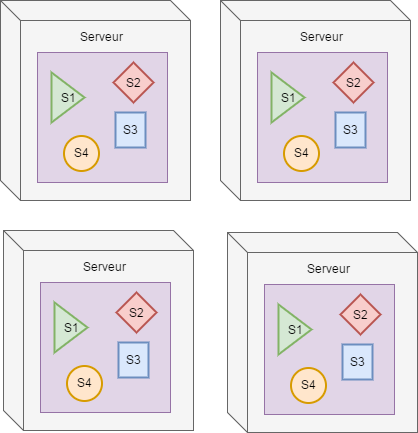
\includegraphics[scale=0.55]{images/travailNeuflizeOBC/architecture/monolithScale.png}
		\caption{Scalabilité horizontale d'une application monolithique \\}
		\label{monolithScale}
    \end{minipage}%
    \hspace{0.5cm}
    \begin{minipage}{.5\textwidth}
        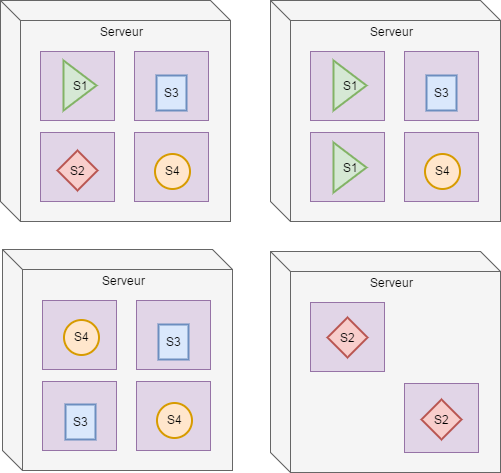
\includegraphics[scale=0.5]{images/travailNeuflizeOBC/architecture/microservicesScale.png}
		\caption{Scalabilité horizontale des microservices \\}
		\label{microservicesScale}
    \end{minipage}
\end{figure}

		Dans notre cas, l'objectif de la couche microservices , située dans le tiers 2, est de réaliser la composition des services métiers exposés par EFS dans le but d'exposer les données pour les applications ou les partenaires (comme PBI dont nous avons parlé dans la partie \ref{prezAppNeuflize}) qui viendront les consommer. Cette dernière est constituée des éléments présents sur la figure \ref{coucheMicroservices}. Les services EFS sont exposés via une surcouche API, située dans le tiers 2. \\

\begin{figure}[h!]
\raggedleft
	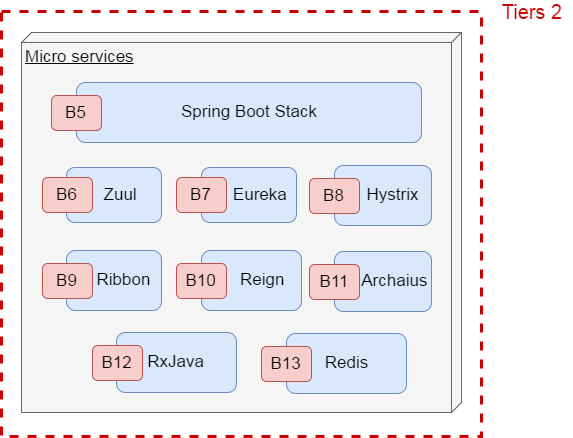
\includegraphics[scale=0.5]{images/travailNeuflizeOBC/architecture/coucheMicroservices.png}
	\centering
	\caption{Couche microservices}
	\label{coucheMicroservices}
\end{figure}
	
	\textit{Spring Boot Stack} est la brique applicative hébergeant les microservices. C’est dans cette dernière que la composition de services EFS est réalisée. Spring boot permet d'utiliser le framework java \textit{Spring} en simplifiant grandement la configuration, le déploiement ou encore la sécurité et en créant des applications cloud-ready.
	Cette brique prend aussi en charge l’implémentation des principaux patterns à savoir : \\
	
\begin{itemize}
	\item Circuit breaker : Capacité du système à être tolérant à la panne. En cas d’erreur successive lors de l’appel d’un sous-composant, le circuit d’appel est coupé « temporairement » en adoptant un comportement par défaut. L'implémentation qui a été choisie pour ce pattern est Hystrix de la stack \textit{Netflix OSS} \cite{bib_hystrix} permettant de contrôler la latence et les erreurs dues à des appels réseaux. L'idée essentielle est d'empêcher les erreurs en cascade dans un environnement distribué. Hystrix permet de \textit{fail-fast} mais de se rétablir rapidement créant ainsi une architecture tolérante aux erreurs capable de se remettre de manière autonome (on parle de self-heal). Ainsi, dès sa conception, le système prévoit les pannes.
	\item Feature toggle : Le principe est d’avoir une branche de développement et de déployer en production en continu. Ensuite, l’activation d’une « feature » est pilotée par le business. Cela permet aussi d’activer une fonctionnalité en fonction d’une population ou une stratégie particulière. \\
\end{itemize}

	Le serveur d'annuaire, essentielle à une architceture distribuée, permet la détection automatique des instances déployées. Les instances des applications sont accédées via leur nom (par exemple account-service) plutôt que par leurs adresses physiques/IPs. Les applications n'ont plus besoin de connaitre les adresses des instances. L'implémentation de l'annuaire de service est Eureka de la stack \textit{Netflix OSS} \cite{bib_eureka}. Les applications clientes peuvent s'enregistrer sur Eureka, via une annotation, qui fournira des metadatas telles que l'URL, le port ou encore le fil de vie (healthcheck) des instances. Eureka reçoit des messages dits "heartbeat" provenant de ces applications, si aucun message n'est reçu, en fonction d'un temps configurable, il supprimera l'instance. \\

	Ensuite, le point d'entrée unique de l'architecture microservices est sa gateway fournissant des services de routage dynamique, surveillance, résilience et sécurité. L'implémentation choisie est Zuul de la stack \textit{Netflix OSS} \cite{bib_zuul}. L'affichage d'une page web ou mobile peut nécessiter l'appel à une dizaine de microservices différents. Il n'est pas envisageable pour l'application cliente de connaitre l'ensemble des adresses physiques des microservices. Pour répondre à cette problématique, la gateway devient la seule adresse à connaitre pour les applications clientes. Zuul est aussi utilisé pour router les requêtes vers les services adéquats. Celui-ci retrouve les adresses des services automatiquement en interrogeant Eureka. Cependant, les services EFS et d'authentification (Axway gateway) sont paramétrés manuellement puisqu'ils ne sont pas enregistrés sur Eureka. La charge sera ensuite répartie grâce à un autre outils de Netflix, Ribbon, qui fourni des fonctionnalités de load-balancing permettant de distribuer la charge de travail. \\

\section{Déroulement du projet}
		Sur ce projet j'ai été positionné en tant que développeur et ai donc travaillé directement avec l'équipe sur le développement du Fronting Digital. Ainsi, contrairement au projet mené chez Neuflize OBC, je n'ai pas réalisé différents travaux indépendants mais j'ai directement participé au développement de l'application. Cependant, nous avons adopté des méthodes agiles \cite{bib_agile} dont je vais parler plus en profondeur ci-dessous c'est pourquoi je ne peux pas détailler l'ensemble des tâches que j'ai effectuées, ces dernières étant nombreuses et toujours réalisées de la même façon au cours des différents sprints. Aussi, je vais plutôt d'abord expliciter le déroulement de ces sprints ainsi que la manière dont nous avons réalisé la conception des fonctionnalités ensuite de quoi je présenterai certaines tâches que j'ai effectuées en autonomie.

\subsection{Méthodes agiles}
	Comme nous l'avons dit plus haut, nous avons recours à un courant agile \cite{bib_agile2} pour la réalisation de ce projet. Il s'agit d'une approche de gestion de projet qui vient s'opposer aux méthodes plus traditionnelles et séquentielles comme le \textit{cycle en V}. Ces pratiques traditionnelles sont le plus souvent dîtes de \textit{projet au forfait} où l'on établi en début de projet l'ensemble des relations commerciales et des obligations de chaque partie. L'intégralité du produit doit être spécifiée et plannifiée dans les détails ce qui aboutit à la création d'un cahier des charges très conséquent qui sera par la suite confié à l'équipe de développement. Après cela, les développeurs s'isolent sur une très grande période afin de déchiffrer ce cahier et de réaliser le produit. Le client doit avoir pensé à absolument tout, de la disposition des pages de son application à la couleur des boutons des formulaires. Les changements nécessites des avenants et sont réalisés souvent trop tard ce qui est contre-productif. De plus, tous les imprévus rencontrés lors de la phase de développement ont tendance à rendre la plannification de départ obsolète. \\
	
	Les méthodes agiles sont centrées sur la satisfaction du besoin client plutôt que sur la conformité d'un contrat et favorise un raisonnement "produit" plutôt qu'un raisonnement "projet". L'objectif est de ne mettre en place que des cycles courts nommés itérations et de découper le projet en plein de petits blocs. Le demandeur commence par exprimer ses exigences qu'il soumet aux développeurs en communicant directement avec eux, ce qui favorise l'entente et les relations et permet de gagner du temps. L'équipe choisit alors une partie des exigences ainsi qu'une courte période de temps pour effectuer les phases de spécification, conception, developpement et test, au terme de laquelle le produit est montré au client. Celui-ci peut alors émettre des feedbacks offrant de la \textbf{visibilité} qui seront pris en compte par l'équipe de développement. Cela favorise grandement l'entente et surtout la satisfaction du client c'est pourquoi il est crucial d'autoriser le changement. Ainsi, il est possible de s'\textbf{adapter} aux souhaits du demandeur, remplacer une fonctionnalité par une autre, modifier des styles, déplacer une page etc... et de réduire considérablement l'effet tunnel des approches classiques. En effet, il est possible d'éviter le surplus, les fonctionnalités qui ne seront finalement pas utilisées, de mettre en place les bonnes idées apparues pendant le projet et donc de véritablement enrichir le produit en mettant en avant la production de valeur pour l'utilisateur final (on parle de \textbf{business value}). Les \textbf{risques} repérés peuvent etre traités beaucoup plus tôt en travaillant directement avec le demandeur. 
	
\begin{figure}[h!]
	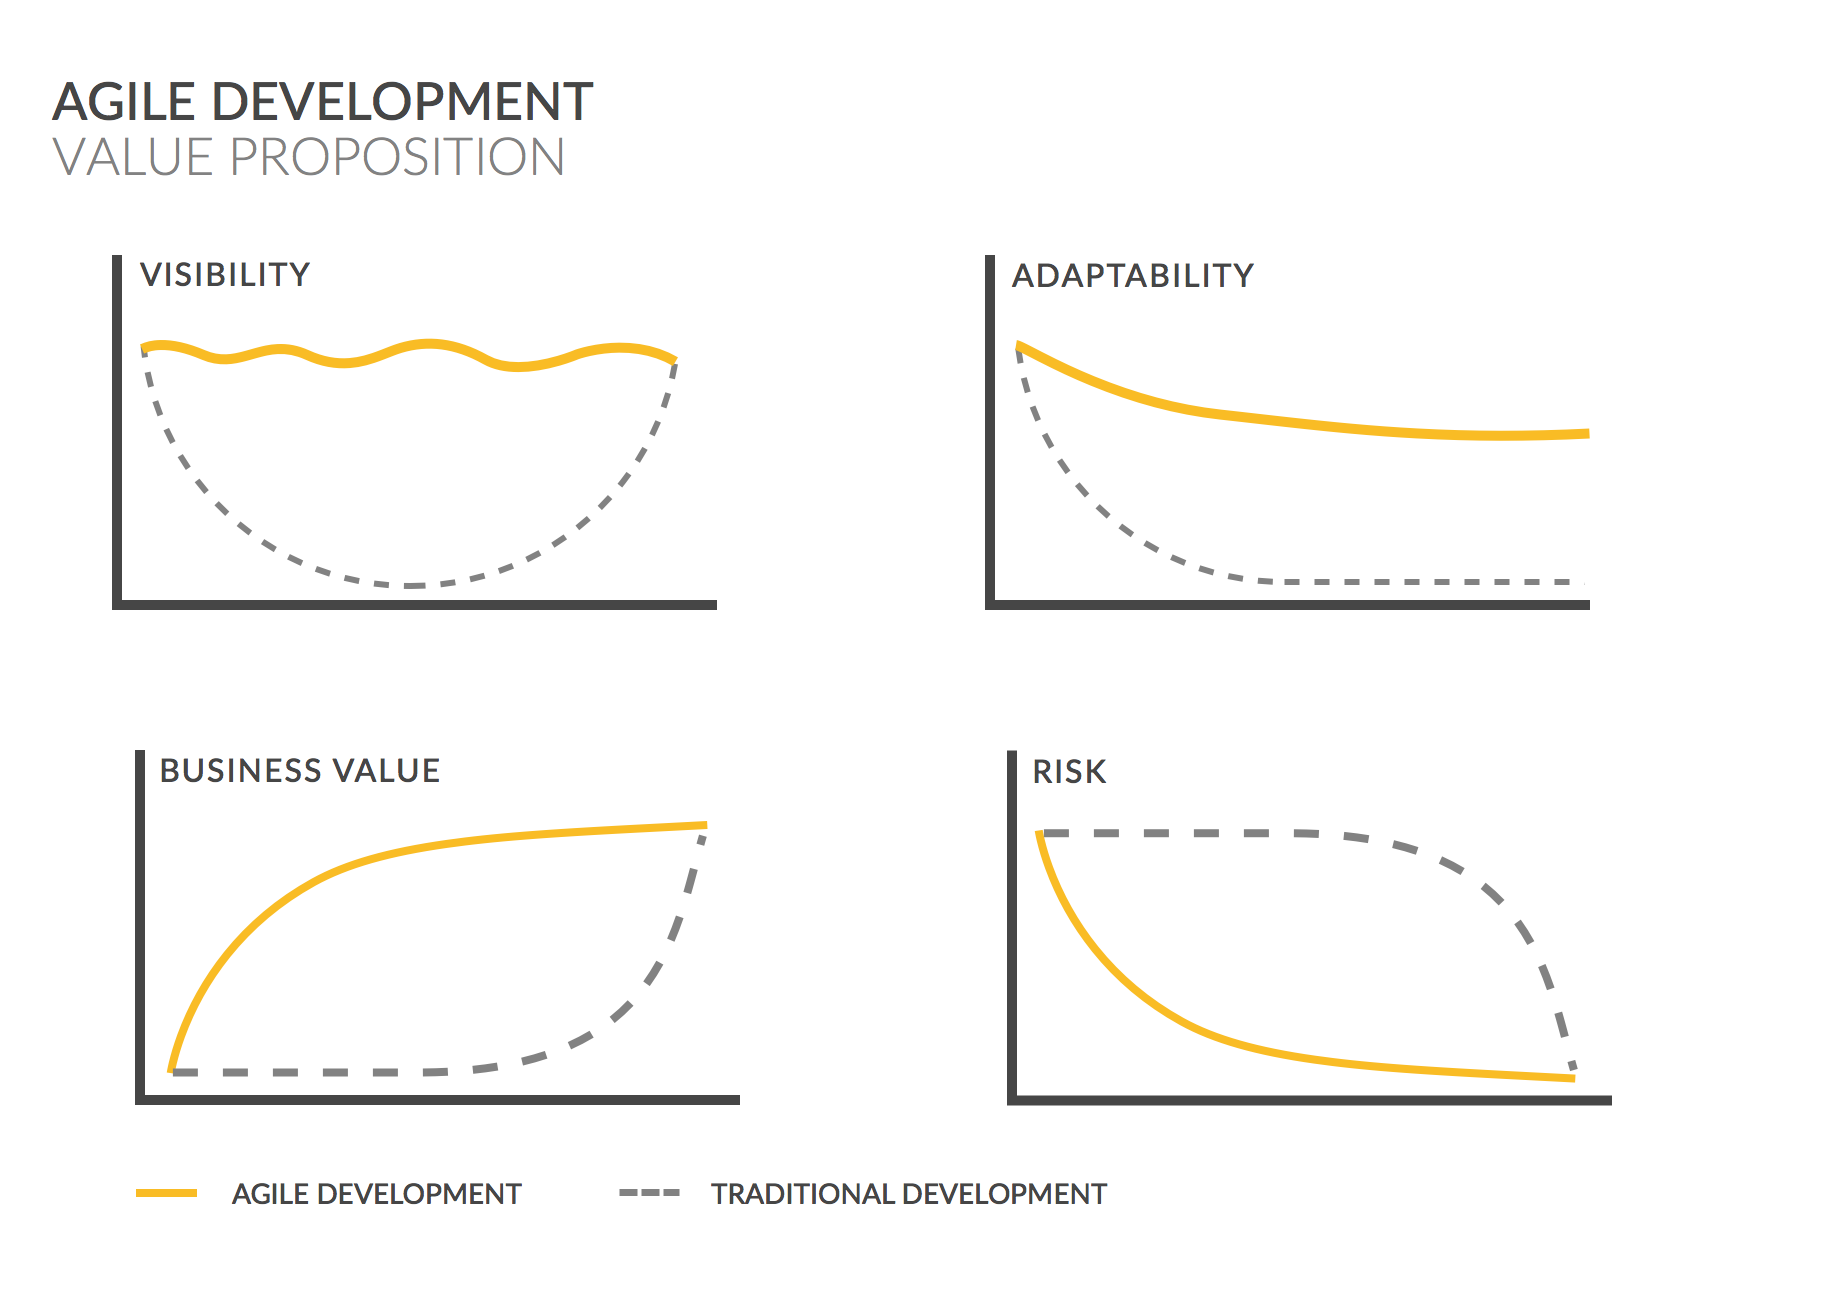
\includegraphics[scale=0.25]{images/travailBP1818/agile.png}
	\centering
	\caption{Comparaison méthodes agiles - traditionnelles}
	\label{agile}
\end{figure}

	Dans notre cas, nous utilisons la méthodologie \textit{Scrum} \cite{bib_agile3}. Il s'agit de l'une des méthodes agiles les plus utilisée dont nous allons maintenant voir le détail.

\subsection{Déroulement des sprints}
\label{deroulementSprint}

	Scrum est une méthode de gestion de projet très répandue et prisée des adeptes de la philosophie Agile. Bien qu'elle soit plutôt simple à comprendre, elle reste néanmoins difficile à mettre en place et à maîtriser dans un projet. \\
	
	\subsubsection{Sprints}
	Nous avons vu plus haut que les méthodes Agiles préconisent de découper la réalisation du projet en un ensemble d'itérations courtes. Ici, ces dernières sont nommées \textbf{sprints} qui sont des périodes de deux semaines (ou parfois trois semaines lorsque des conditions particulières l'imposent comme une diminution des ressources à cause des vacances).
	
	\subsubsection{Le Product Backlog}
	Le product backlog est un référentiel contenant les exigences fonctionnelles et non foncitonnelles initiales définies par le client. Celui-ci est amené à évoluer à mesure que le projet avance.
	
	\subsubsection{User Story}
	Une user story, ou récit utilisateur, est la description d'une fonctionnalité métier à valeur business. Dans notre cas, il s'agit d'un fichier excel décrivant une fonctionnalité du point de vue utilisateur (\textit{En tant que..., je clique sur … dans le but de …}). Elle présente toutes les règles de gestions, prévoit tous les cas d'utilisation et contient aussi des maquettes afin que nous puissions construire l'IHM dans les meilleures conditions possibles.
	
	\subsubsection{Les rôles clés}
	Scrum définit différents rôles clés qui sont les suivants :
	\begin{itemize}
		\item Le \textbf{Product Owner} qui possède une vision globale sur le projet et dont l'objectif est de décrire et prioriser les élements du Product Backlog.
		\item Le \textbf{Scrum Master} dont l'objectif principal est s'assurer que la méthodologie Scrum est correctement appliquée et que ses valeurs sont intégrées par l'équipe.
		\item L'\textbf{équipe} qui se charge de réaliser le produit et donc ici le Fronting Digital
	\end{itemize}
	
	\subsubsection{Déroulement d'un sprint}
	Nos ressources se décomposent en une équipe fonctionnelle, de pilotage ainsi que de développement. Lors d'un sprint, l'équipe fonctionnelle collabore avec les métiers BP1818 et le product owner afin de pouvoir constituer un backlog suffisamment complet et ordonnancé pour plannifier le prochain sprint. Pour cela des \textbf{ateliers} sont régulièrement organisés entre ces deux parties afin de faire constamment évoluer le product backlog. Après cela, cette équipe est en charge de rédiger les \textbf{User Stories}. Une user story représente une exigence ou une fonctionnalité souhaitée par le client et décrit celle-ci de manière détaillée en précisant le comportement attendu, des maquettes pour l'IHM etc... : \textit{Lorsque je vais sur la page ... et que je clique sur le bouton ... l'action ... se déclenchera}. \\
	
	Une fois ces dernières validées, elles nous sont transmises, côté équipe de développement, afin que nous puissions les étudier. Dans un premier temps, l’ensemble de l’user story est découpée en tâches unitaires pouvant être réalisées par une unique ressource, qui seront consignées sous forme d’issue sous Github. Par la suite, une réunion de type \textbf{Sprint Planning} est organisée avec l'ensemble de l'équipe Sopra Steria dans l’optique de valider le contenu du sprint. Lors de ce sprint planning nous présentons l’ensemble des tâches découpées précédemment à l’équipe et exposons brièvement la manière dont nous les développerons afin que chacun puisse s’imprégner du travail qui sera réalisé et que les dernières modifications puissent être apportées. Ensuite, pour chacune des tâches ainsi dévoilées, une estimation de charge est réalisée via la méthode du \textbf{Poker Planning}. Il s’agit d’une pratique permettant d’estimer la complexité des fonctionnalités à développer en faisant interagir de manière ludique l’ensemble des parties prenantes. En effet, chaque participant possède des cartes indiquant différents niveaux de complexité (les niveaux représentent les nombres de la suite de Fibonacci). Lorsqu’une des tâches a été présentée par les développeurs, les participants choisissent la carte correspondant à leur estimation personnelle de la compléxité et la retourne tous en même temps. La discussion reprend tant qu’il n’y a pas l’unanimité sur la valeur de la complexité. Dans notre cas, un point de compléxité correspond à 0.75 jour de travail pour une ressource. Par exemple, si une tâche est validée à 5 points de complexité alors cette dernière devra être réalisée en 3.75 jours. Une fois les estimations terminées, certaines tâches sont choisies en fonction de leur priorité définie avec le product owner et du temps disponible pour le sprint et constituront le \textbf{Sprint Backlog}.\\
	
	A l'issue de cette réunion la phase de développement peut commencer. Elle inclut la conception détaillée des différentes tâches, le développement ainsi que les tests unitaires. Lorsque le développement est terminé le produit partiel est livré et part en phase de qualification. Cette phase est menée par l'équipe fonctionelle qui sera en charge d'effectuer toute une batterie de test afin de vérifier la conformité du produit à l'user story. Tous les bugs relevés sont consignés sous forme d'issue sur Github afin que nous puissions les corriger. Cette phase est en quelque sorte une phase de pré-recette nous permettant de nous affranchir d'un maximum d'anomalies avant de livrer l'application aux métiers.

\begin{figure}[h!]
	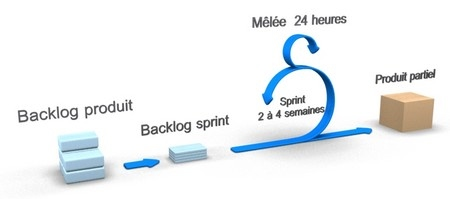
\includegraphics[scale=0.7]{images/travailBP1818/scrum.jpg}
	\centering
	\caption{Méthode Scrum}
	\label{scrum}
\end{figure}

	Une réunion nommée \textit{Daily meeting} a lieue chaque jour dans le but de vérifier que les objectifs seront bien atteints. Lors de cette réunion le but est de répondre aux trois questions suivantes : 
	\begin{itemize}
		\item Qu'est-ce que j'ai fait ?
		\item Qu'est-ce que je vais faire ?
		\item Quels sont les problèmes que je rencontre ?
	\end{itemize}
	Elle regroupe l'ensemble des équipes intervenant sur le projet à savoir Sopra Steria, la DSI ainsi que les métiers et dure 15 minutes. Un second daily meeting a lieu juste après, lui aussi de 15 minutes mais seulement avec l'équipe Sopra Steria. \\

	En outre, une fois par semaine a lieue une réunion nommée \textit{V1} ne concernant elle aussi que l'équipe Sopra Steria et dans laquelle un bilan est effectué concernant l'avancement du projet, les problèmes majeurs rencontrés, les retards possibles, les mesures à prendre etc... Cette dernière est présidée par notre directeur de projet. \\
	
	Personnellement, je trouve que l'ensemble de ces réunions permet de soulever les problèmes et favorise la collaboration en permettant à tout le monde d'invervenir et de proposer ses idées. Cependant, leur trop grand nombre implique une grande perte de temps, temps souvent précieux pour l'équipe de développement. Durant le daily meeting de Sopra Steria nous parlons en détail du développement et de l'application. Or, nous ne pouvons aborder ces points techniques durant celui avec les métiers. Lors du daily métier, il est fréquent que seul les points métiers soient évoqués, points dont l'équipe de développement ne saisi pas forcément le sens. De plus, il n'est pas rare que le temps réglementaire de 15 minutes soit dépassé. \\
	
	Concernant les sprint planning, il s'agit d'une réunion très intéressante permettant d'estimer la charge en faisant, là aussi, intervenir tout le monde. Néanmoins, il est fréquent que le temps alloué à cette dernière soit dépassé, voire parfois nettement dépassé. En effet, le temps peut parfois atteindre jusqu'à 3h. Cela est dû au fait que nous n'avons jamais de \textit{time keeper} ou gardien du temps afin d'aiguiller la réunion. Parfois d'autre points sont abordés lors de la réunion et certaines digressions font perdre du temps. Le temps total passé en réunion est souvent supérieur à ce qu'il aurait dû être et manque à la phase de développement. \\
	
	Enfin, une fois la phase de qualification terminée et le projet partiel livré au client, une réunion \textit{Sprint review} est organisée avec l'ensemble de l'équipe de projet et est dirigée par l'équipe fonctionnelle Sopra Steria. Son objectif est de présenter ce qui a été développé au cours du sprint au client et noter les remarques que celui-ci peut être amené à faire. Ces réunions sont un moyen très efficace de communiquer avec le client et nous permettent de prendre en compte ses remarques et idées sur le projet. Elle s'inscrit bien dans le courant agile en favorisant les intéractions entre les différents collaborateurs, en permettant à chacun de s'intégrer au sein du projet et de se sentir acteur dans le cadre du Fronting Digital. Il s'agit là d'un point que j'ai particulièrement apprécié au sein de l'équipe, balayant les préjugés classiques sur les gros projets tels que la phase d'isolement des développeurs après l'établissement des spécifications. Ici la communication est au coeur de la réussite du projet et permet d'assurer un résultat conforme aux besoins et aux attentes du client, même si ces dernières évoluent au cours du temps.
	
\section{Moteur de scoring MIF}
	\label{moteurScoring}
	\subsection{Etude du besoin}
	\input{src/travailBP1818/moteurScoring/moteurScoring_01}

\subsection{Backend}
	\input{src/travailBP1818/moteurScoring/moteurScoring_02}
	
\subsection{Frontend}
	\input{src/travailBP1818/moteurScoring/moteurScoring_03}
	
\section{Recherche client}
	\input{src/travailBP1818/rechercheClient}
	
\section{Pièces justificatives}
	\subsection{Etude de l'user story}

	Le Fronting Digital est avant tout une application destiné aux banquiers afin de leur permettre de gérer plus efficacement et facilement leurs entrées en relation. Or, lors d'une ouverture de compte ou d'une souscription à une assurance vie il est obligatoire de fournir certains documents comme une pièce d'identité, un relevé d'identité bancaire ou encore un justificatif de domicile. Ici, ces documents sont appelés "pièces justificatives" et ont fait l'objet d'une user story sur laquelle j'ai travaillé de manière autonome, coinjointement avec un autre stagiaire. \\
	
	Le contenu de cette story concernait la mise en place d'un nouvel écran sur l'application depuis lequel il est possible d'uploader/downloader des pièces justificatives. Les pièces obligatoires qui doivent être fournies par le futur client de la banque dépendent de ses données personnelles. Par exemple, un client personne physique mineur ne fournira pas les même pièces qu'un client personne morale. Ainsi, le nouvel écran doit pré-afficher la liste des pièces obligatoires en la calculant au préalable à partir des données saisies par le banquier. La story mettait à notre disposition une matrice définissant l'ensemble des règles de gestion permettant de déterminer, à partir des données, si une pièce était obligatoire ou non. De plus, l'écran doit aussi proposer un menu déroulant permettant de choisir n'importe quel type de pièce afin de l'ajouter manuellement à la liste. Les pièces ajoutées de cette manière sont facultatives et doivent être affichées d'une couleur différente. Il est possible de retrouver en annexe \ref{frontingDigitalPJ} une maquette illustrant ce nouvel écran. \\

	Comme nous l'avons expliqué dans la partie \ref{deroulementSprint}, la première étape pour l'équipe de développement consiste à prendre connaissance de l'user story afin de la découper en tâches unitaires. Ici, nous avons fait le choix de créer 5 tâches qui sont les suivantes :
	
	\subsubsection{Composant pièce justificative}
	Le composant "pièce justificative" est un composant Angular représentant la brique qui contient tous les éléments et options d'une pièce justificative à savoir :
	\begin{itemize}
		\item Le fichier
		\item La date de fin de validité
		\item L'accord dérogatoire
		\item La date d'upload du fichier
		\item La possibilité de supprimer la pièce
		\item La possibilité de visualiser la pièce (ou la télécharger si elle ne peut être visualiser sur le navigateur)
	\end{itemize}
	Cette brique est représentée par un rectangle rouge sur l'annexe \ref{frontingDigitalPJ}
	
	\subsubsection{Composant écran pièce justificative}
	Ce composant est l'écran sur lequel sont affichées les pièces justificatives sous la forme d'une liste dont les éléments sont les composants décrits précédemment. Celui-ci pré-remplie la liste avec les pièces définies comme étant obligatoires. Ainsi, le banquier aura un rapide aperçu des pièces qu'il doit demander à son client et n'aura qu'à uploader les fichiers pour compléter la liste. De plus, un menu déroulant doit être présent, permettant de rajouter des pièces manuellement à la liste, dites facultatives qui apparaissent d'une couleur différente. En outre, le service d'appel front devra être créé afin de pouvoir communiquer avec l'API et consommer les web services. En outre, l'écran doit être accessible depuis la barre de navigation principale de l'application et un compteur indiquant le nombre de pièces obligatoires fournies/totales (par exemple 2/5) doit figurer au-dessus de la barre.
	
	\subsubsection{Référentiel}
	Dans notre application apparait un certain nombre de données métiers constantes comme la liste des pays pour un client, la liste des départements pour la France ou encore la liste des formes juridiques pour une entreprise. Pour toutes ces listes de données un endpoint est ajouté et un service appelé \textit{référentiel} est créé. Ainsi, il est possible de les obtenir de manière simple depuis le front en consommant le service adéquat. Si les métiers ont le besoin de modifier les valeurs, il suffit d'apporter une simple modification rapide et cela permet de garder un code structuré et clair. Dans notre cas, un référentiel devait être créé afin de référencer tous les types de pièces justificatives prises en charge par la banque (carte d'identité, justificatif de domicile, etc... pour un total de 41 différentes).	
	
	\subsubsection{Backend}
	Comme son nom l'indique, cette tâche consiste à développer les services backend destinés à alimenter notre frontend. Cela implique la création du contrôleur et de tous les endpoints, le service dédié ainsi que le modèle permettant de gérer les pièces justificatives. De plus, cela inclut le paramétrage pour la limite de taille des fichiers à uploader ainsi que la validation des données reçues.
	
	\subsubsection{Moteur de calcul}
	Nous avons dit plus haut que l'écran des pièces dévait pré-afficher la liste des pièces obligatoires. Or, le fait qu'une pièce soit obligatoire ou non dépend des données personnelles du client de la banque. Ainsi, le moteur de calcul doit prendre en compte l'ensemble des règles de gestion métiers ainsi que les données entrées jusqu'à présent par le banquier dans l'application afin de définir la liste des pièces obligatoires puis la transmettre au composant écran. \\
	
	Comme je l'ai dit plus haut, j'ai travaillé sur cette story avec un autre stagiaire. Ainsi, nous nous sommes séparé les tâches avant de commencer c'est pourquoi je me suis plutôt occupé de la partie backend et lui de la partie frontend. Ce découpage permettait d'avancer en parallèle sans problèmes. \\
	
\subsection{Sprint planning}
	Après avoir étudier l'user story et définie les différentes tâches à réaliser, une réunion de type sprint planning a eu lieu afin de définir la charge de travail pour effectuer chacune d'entre elles. Au cours de cette réunion nous avons voté et la charge a été réparti de la manière suivante :
	
\begin{table}[h!]
	\center
	\begin{tabular}{| c | c |}
     \hline
     Tâche & Charge (jour) \\ \hline
     Composant pièce justificative & 3.75\\ \hline
     Composant écran justificatifs & 3.75\\ \hline
     Backend & 2.25\\ \hline
     Référentiel & 1.5\\ \hline
     Moteur de calcul & 9.75\\
     \hline
	\end{tabular}
	\caption{Sprint planning pièces justificatives}
	\label{sprintPlanningPJ}
\end{table}

	Une fois le sprint planning terminé nous avons pu passer à la conception de nos tâches respectives ainsi qu'à la phase de développement.

\subsection{Conception backend}

	\subsubsection{Endpoints - couche controller}

	Dans un premier temps, j'ai commencé par définir les différents cas d'utilisation possible d'un banquier qui utiliserait l'écran des pièces justificatives. Il est possible d'observer ces cas sur le diagramme figure \ref{useCasePJ}.

\begin{figure}[h!]
	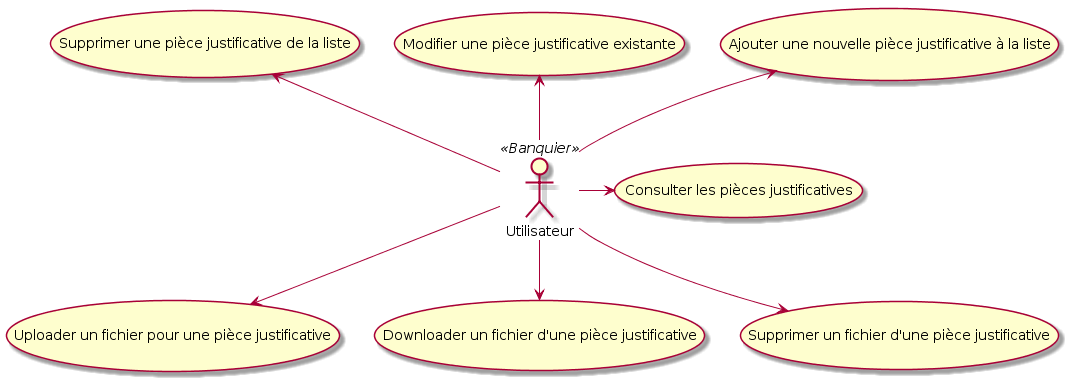
\includegraphics[scale=0.50]{images/travailBP1818/piecesJustif/useCasePJ.png}
	\centering
	\caption{Cas d'utilisation}
	\label{useCasePJ}
\end{figure}

	Pour chacun de ces derniers j'ai décidé de mettre en place un service permettant de répondre au besoin qu'il définissait. J'ai ainsi pu procéder à la création du contrôleur ainsi que des endpoints permettant d'exposer les services répondant aux cas d'utilisation. Pour cela, il a fallu déterminer les méthodes HTTP et l'url associée que notre client pourra intéroger en essayant de rester RESTful. Le tableau suivant décrit les endpoints ainsi créés :
	
\begin{table}[h!]
	\center
	\begin{tabular}{| c | c | c |}
     \hline
     Cas d'utilisation & Méthode HTTP & URL \\ \hline
     Obtenir pièces justificatives & GET & /justificatifs/{idForm}\\ \hline
     Créer pièce justificative & POST & /justificatifs/{idForm}/justificatif\\ \hline
     Modifier pièce justificatives & PUT & /justificatifs/{idForm}/justificatif\\ \hline
     Supprimer pièce justificative & DELETE & /justificatifs/{idForm}/justificatif\\ \hline
     Downloader fichier & GET & /{idForm}/fichier\\ \hline
     Uploader fichier & POST & /{idForm}/fichier\\ \hline
     Supprimer fichier & DELETE & /{idForm}/fichier\\ \hline
	\end{tabular}
	\caption{Sprint planning pièces justificatives}
	\label{sprintPlanningPJ}
\end{table}

	En outre, j'ai créé un endpoint supplémentaire que j'ai placé dans le contrôleur \textit{ReferentielController} dédié aux référentiels. Celui-ci permet d'accéder au référentiel des pièces justificatives et donc d'obtenir la liste des types de pièces qu'il est possible d'utiliser dans l'application.

	\subsubsection{Modèle - couche domain}
	
	Comme nous l'avons vu dans la partie \ref{archiBP1818}, nous avons recours à Couchbase pour notre base de données de type NoSQL. Ainsi, toutes les données sont enregistrées sous la forme de documents au format JSON. Dans notre cas, nous avons généralement un document par formulaire dont le nom est constitué de l'id du client et d'un préfixe permettant d'identifier rapidement le formulaire. Par exemple, nous avons un écran sur lequel il est possible de spécifier les données personnelles du client. Le formulaire est sauvegardé dans un document portant le nom \textit{TIERS\_10001} pour le client d'id 10001. Nous avons un écran déroulant une série de questions sur les patrimoines et revenus du client. Le formulaire regroupe les réponses à toutes les questions et est sauvegardé dans le document \textit{PAT\_10001}, toujours pour le client d'id 10001. Ainsi, dans le cas des pièces justificatives j'ai décidé de sauvegarder l'ensemble du formulaire contenant les pièces dans un nouveau document dont le nom serait \textit{JUST\_ID}. \\
	
	Une fois cela définit, il fallait déterminer quelles données devaient être persistées ainsi que leur structure. J'ai donc commencé par définir le modèle qui serait utilisé en étudiant plus en profondeur l'user story afin de relever toutes les informations à persister. Ce modèle peut être représenter par le diagramme de classe figure \ref{modelePJ}.	
	
\begin{figure}[h!]
	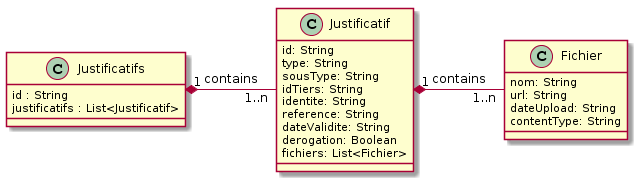
\includegraphics[scale=0.7]{images/travailBP1818/piecesJustif/modelePJ.png}
	\centering
	\caption{Modèle des pièces justificatives}
	\label{modelePJ}
\end{figure}

	La classe \textit{Fichier} représente un fichier uploadé par le banquier et contient ses informations comme son nom, l'url indiquant à quel endroit est enregistré le fichier, la date à laquelle il a été enregistré et son content-type. Celui-ci est une en-tête permettant d'indiquer le type MIME d'une ressource, nécessaire dans notre cas pour visualiser le fichier dans le navigateur. \\
	
	Ensuite, la classe \textit{Justificatif} représente une pièce justificative et toutes les informations qui lui sont associées comme le type ou la date de validité. Elle contient aussi l'id du tiers ("idTiers") à qui elle appartient afin de pouvoir l'identifier ainsi que son identité ("identite") afin de pouvoir afficher le nom de son propriétaire côté frontend (par exemple carte d'identité de M. Jean Dupont). En outre, cette classe contient une liste de fichier ("fichiers") contenant tous les fichiers uploadés pour la pièce justificative (par exemple pour une carte d'identité il peut y avoir deux fichiers : une image pour le recto et une pour le verso). \\
	
	Enfin, la classe \textit{Justificatifs} contenant l'id du document au format JUST\_ID ainsi qu'une liste de pièces justificatives ("justificatifs"). \\
	
	J'ai pu implémenter ce modèle en Java en créant des Beans côté backend. Nous utilisons actuellement Maven comme outil de gestion et d'automatisation de production de logiciel. Nous avons configuré un plugin Maven, nommé \textit{Typescript Generator}, permettant de générer le modèle côté frontend. En effet, une fois le modèle créé côté backend, il suffit de relancer un build Maven afin que ce plugin génère le code Typescript à partir du code Java. Un fichier est créé contenant toutes les interfaces typescript obtenues à partir des Beans java. Cela nous permet d'assurer la cohérence entre nos modèles back et front et nous permet de gagner beaucoup de temps en nous évitant de réécrire une seconde fois le modèle.
	  
	
	\subsubsection{Communication avec Couchbase - couche repository}
	
	Le modèle étant défini, il fallait maintenant mettre en place la communication avec Couchbase afin de persister les données ou les récupérer. Pour cela, j'ai créé un repository pour les pièces justificatives. Comme nous l'avons vu plus haut, il s'agit d'une interface facilitant grandement l'utilisation de requêtes vers notre base de données. Le schéma figure \ref{repository} illustre le fonctionnement du repository des pièces justificatives. \\
	
	J'ai donc créé JustificatifsRepository et fait en sorte que la classe \textit{Justificatifs} implémente l'interface IdentifiableDocument. Pour cette user story aucune autre requête que celles fournies était nécessaire donc aucun développement supplémentaire était requis. \\

\begin{figure}[h!]
	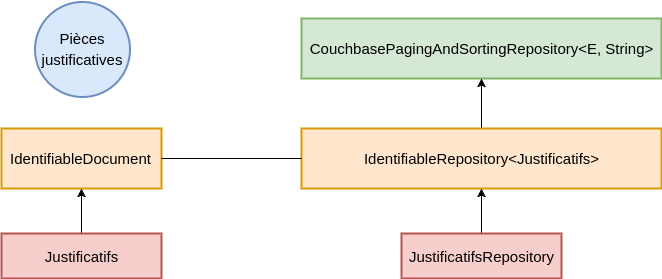
\includegraphics[scale=0.55]{images/travailBP1818/piecesJustif/repositoryPJ.png}
	\centering
	\caption{Repository pièces justificatives}
	\label{repositoryPJ}
\end{figure}
		
	\subsubsection{Service - couche service}
	
	A ce stade, les cas d'utilisation étaient connus, le modèle défini, la communication avec Couchbase établie et les endpoints exposant les services prêts. La prochaine étape consistait à effectivement développer les services permettant de répondre aux différents besoins identifiés sur le diagramme figure \ref{useCasePJ}.
	
\begin{table}[h!]
	\center
	\begin{tabular}{| c | c |}
     \hline
     Services & Description \\ \hline
     findJustificatifs & Permet de retourner le formulaire JUST\_ID contenant toutes les pièces \\ \hline
     createPiece & Permet de créer pièce justificative en l'ajoutant au formulaire \\ \hline
     updatePiece & Permet de mettre à jour une pièce justificative du formulaire \\ \hline
     deletePiece & Permet de supprimer une pièce justificative en la supprimant du formulaire \\ \hline
     uploadFile & Permet d'uploader un fichier \\ \hline
     downloadFile & Permet de downloader un fichier \\ \hline
     deleteFile & Permet de supprimer un fichier\\ \hline
	\end{tabular}
	\caption{Services pièces justificatives}
	\label{servicesPJ}
\end{table}

	Comme nous l'avons expliqué, l'écran des pièces justificatives doit présenter la liste des pièces obligatoires obtenu par le biais du moteur de calcul. Pour chacune de ces pièces il est possible d'ajouter un ou plusieurs fichiers en appelant le service uploadFile. Comme il est possible de l'observer sur le diagramme figure \ref{seqSave} et à la demande des métiers, une pièce est sauvegardée si et seulement si elle possède un fichier. Dans le cas contraire la pièce n'est pas ajoutée au formulaire qui sera envoyé au back par la suite et ne sera donc pas sauvegardée. En effet, si une pièce obligatoire ne possède pas de fichier elle sera simplement ajoutée par le moteur de calcul implémenté côté front. Concernant les pièces facultatives, il est logique qu'elles ne soient pas sauvegardées si aucun fichier n'est ajouté. A chaque fois qu'un fichier est ajouté à une pièce, une requête POST est envoyée via le service createPiece afin de créer la pièce côté back s'il s'agit de son premier fichier sinon une requête PUT est envoyée via le service updatePiece afin de mettre à jour le formulaire des pièces justificatives. \\

\begin{figure}[h!]
	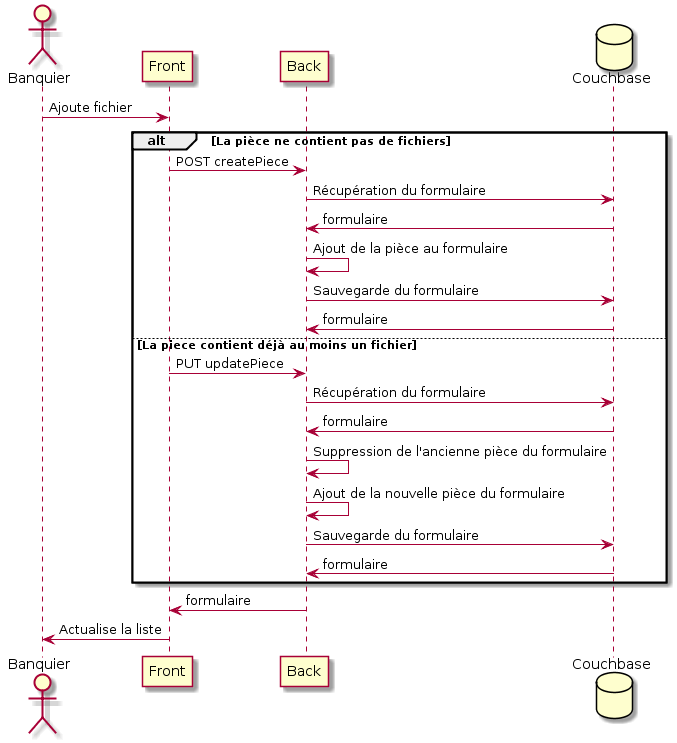
\includegraphics[scale=0.55]{images/travailBP1818/piecesJustif/seqSave.png}
	\centering
	\caption{Sauvegarde des pièces justificatives}
	\label{seqSave}
\end{figure}

	Ensuite, lorsque l'utilisateur souhaite accéder à l'écran des pièces justificatives, le moteur de calcul fourni la liste des pièces obligatoires pendant qu'une requête est envoyée côté back via le service findJustificatifs pour récupérer le formulaire contenant toutes les pièces sauvegardées de manière asynchrone. Une fois les deux listes obtenues, elles sont mergées en une liste finale afin d'éliminer les doublons qui sera affichée sur l'écran. Par exemple, le moteur peut indiquer que la pièce "carte d'identité" est obligatoire. Si les fichier de la carte d'identité du titulaire du compte ont bien été ajouté et sauvegardé alors lors du merge de la liste du moteur et de la liste du back, seule la pièce "carte d'identité" du back sera gardée. Le diagramme de séquence réalisé pour ce cas figure \ref{seqGet} illustre ce principe. En sauvegardant et récupérant les pièces de cette manière nous pouvons maintenir la cohérence des données et limiter le nombre de requêtes envoyées à notre backend. \\
	
	Les autres services comme le téléchargement de fichiers ou la suppression de pièces n'ont pas nécessité de diagrammes et sont utilisés simplement par clic sur un bouton. \\

\begin{figure}[h!]
	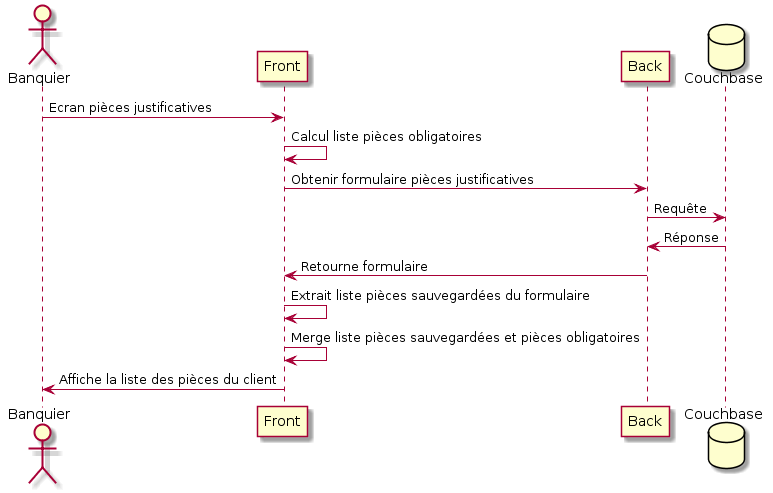
\includegraphics[scale=0.55]{images/travailBP1818/piecesJustif/seqGet.png}
	\centering
	\caption{Affichage des pièces justificatives}
	\label{seqGet}
\end{figure}

\subsection{Conception frontend}
	
	Pour la partie frontend je me suis chargé de mettre en place le moteur de calcul permettant de fournir la liste des pièces obligatoires pour un client de la banque. Pour cela, j'ai mis en place un service uniquement dédié à ce moteur. L'user story contenait une matrice listant toutes les pièces justificatives acceptées par la banque ainsi que les règles de gestion métiers indiquant si la pièce était obligatoire ou non. Que le client de la banque soit une personne physique ou une personne morale, ces règles n'étaient basées que sur les données personnelles de ce client. De ce fait, le service du moteur ne nécessitait que le formulaire des données personnelles dans le but de fournir la liste des pièces obligatoires. \\
	
	Comme je l'ai expliqué dans la partie \ref{frontendArchi}, nous avons mis en place différents resolver car nous avons parfois le besoin de charger certaines données avant l'initialisation d'un composant. Ainis, ici, j'ai utilisé un resolver dont l'objectif est de récupérer le formulaire contenant les données personnelles du client en intérogeant notre backend. Or, calculer la liste des pièces obligatoires ne suffit pas. En effet, il faut aussi afficher les pièces sauvegardées qui auraient déjà été ajoutées par le banquier en évitant les doublons. \\
	
	Par exemple, admettons que le moteur déclare que la pièce d'identité est obligatoire pour un client. Le banquier upload deux fichiers pour cette pièce (recto et verso de la carte d'identité du client en question). Comme nous l'avons vu, lorsqu'une pièce se voit attribuer un fichier, une requête PUT est envoyée côté back et la pièce est persistée sur Couchbase. Lorsque le banquier se rend à nouveau sur l'écran des pièces justificatives sans faire d'autres modifications sur l'application, le moteur déclarera toujours que la pièce d'identité est obligatoire. Or, cette dernière ayant déjà été complétée, il faut afficher la pièce sauvegardée déjà remplie issue de Couchbase et non pas celle issue du moteur qui est vide. \\
	
	Pour cette raison j'ai dû avoir recours à un second resolver permettant de récupérer le formulaire contant toutes les pièces sauvegardées sur Couchbase. Une fois les formulaires obtenus, ceux-ci sont envoyés au composant qui est alors initialisé. Lors de cette initialisation, le service du moteur de calcul est obtenu par injection de dépendance et calcule, dans un premier temps, la liste des pièces obligatoires puis merge cette liste avec la liste des pièces sauvegardées afin d'éliminer les doublons avant de l'afficher. \\
	
	En outre, l'écran doit proposer un menu déroulant permettant au banquier d'ajouter manuellement n'importe quel type de pièce. La pièce ajoutée ainsi sera alors facultative et apparaitra d'une couleur différente. Cependant, comme nous l'avons vu, les types de pièces sont issus d'un référentiel créé au préalable. Ainsi, lors de l'initialisation du composant, il fallait aussi récupérer la liste des types de pièces depuis ce référentiel. J'ai ici pu tirer profit des possibilités offertes par Angular en matière de programmation asynchrone. En effet, pendant que le composant récupère la liste des pièces qui sera affichée dans le menu déroulant, celui-ci appelle le service du moteur de calcul en parallèle. Cela nous permet de gagner un peu en rapidité et de compenser le temps perdu par les resolvers.

\subsection{Résultats et perspectives}

	Une fois le développement des fonctionnalités terminée, j'ai pu passer au développement des différents tests unitaires dont l'objectif premier est d'éviter les régressions de l'application à mesure que le code évolu. Après cela, le projet partiel est passé en phase de qualification où certaines anomalies ont été relevées avant d'être livré au client. C'est alors qu'une sprint review a eu lieu suivie d'une réunion de sprint planning pour le prochain sprint. Lors de cette réunion, nous commençons par effectuer une rétrospective du sprint précédent. Pour le sprint des pièces justificatives nous avons obtenu les résultats présents sur le tableau \ref{retroPJ}.

\begin{table}[h!]
	\center
	\begin{tabular}{| c | c | c |}
     \hline
     Tâche & Charge prévue (jour) & Charge réelle (jour) \\ \hline
     Composant pièce justificative & 3.75 & 6\\ \hline
     Composant écran justificatifs & 3.75 & 5\\ \hline
     Backend & 2.25 & 5\\ \hline
     Référentiel & 1.5 & 1\\ \hline
     Moteur de calcul & 9.75 & 2\\
     \hline
	\end{tabular}
	\caption{Rétrospective pièces justificatives}
	\label{retroPJ}
\end{table}
	
	Comme on peut l'observer, sur ce sprint, la charge réelle est en grand désaccord avec la charge prévue. Cela est en partie dû à une mauvaise estimation de notre part. Par exemple, j'ai réalisé le moteur de calcul bien plus vite que prévu. Nous avions mal estimé la complexité de cette tâche, ce qui peut être causé soit par une mauvaise compréhension de cette dernière soit par une mauvaise étude de l'user story avant le sprint planning. Cette seconde raison n'est pas à rejeter, il est en effet fréquent que l'équipe de développement soit très occupée par manque de ressource et nous ne disposons parfois que peu de temps pour nous imprégner des stories avant le sprint planning. Ce problème sera désormais réglé puisque deux nouveaux développeurs sont attendus pour la fin juillet. \\
	
	Ensuite, je ne pense pas que la faute concerne uniquement une mauvaise estimation. Certes cette dernière était biaisée mais cette user story était la première que j'ai réalisé en autonomie depuis sa lecture à sa réalisation en passant par sa conception. Il est probable qu'il y ait eu un certain manque de recul de ma part, ce qui m'a obligé à retoucher plusieurs mon modèle et donc ma conception initiale. Afin de pallier cela, je me suis chargé d'effectuer certaines tâches de refactoring dans l'application comme la mise en place d'un système de cache dont je vais parler ci-dessous ainsi que des test sur des fonctionnalités qui n'étaient pas testées pendant quelques jours. Cela m'a permi d'avoir une bien meilleure vision de l'application en explorant les parties du code dont je n'avais jamais pris connaissance tout en permettant de sécuriser le code contre les régressions. \\
	
	Enfin, dernier point qui a été pour moi et mon tuteur le principal problème : le manque de communication. En effet, j'ai travaillé avec un autre stagiaire sur cette story. Je me suis chargé du backend, du référentiel et du moteur de calcul pendant que lui s'occupait des composants frontend. Or, celui-ci ignorait que nous possédions un plugin maven générant le modèle frontend à partir du modèle backend et a donc mis en place son propre modèle de son côté. Nous nous sommes rendus compte de cela un peu tard lorsque nous avons commencé à essayer d'intégrer nos travaux et il a donc fallu retoucher le modèle ce qui nous a fait perdre du temps. Aujourd'hui, nous avons une bien meilleure communication et lorsque qu'il est nécessaire de travailler à plusieurs sur une même user story en se séparant les tâches (par exemple un sur le backend et l'autre sur le frontend) nous nous concertons avant et nous parlons dès que le modèle doit évoluer afin que l'autre soit toujours au courant et puisse rester cohérent. \\

	J'ai ici pris le sprint des pièces justificatives en guide d'exemple dans le but d'illustrer l'étude des spécifications, la conception ainsi que la réalisation d'un sprint de manière générale. L'ensemble des sprints se déroule de cette manière sur des périodes de deux à trois semaines selon les conditions et la charge de travail. Je ne décrirais pas plus en profondeur les autres sprints puisque le principe reste le même. Cependant, au cours de ces derniers j'ai parfois été amené à effectuer certaines tâches s'écartant des user stories. Par exemple, nous travaillons le code de manière incrémentale se qui implique des changements et des évolutions. De plus, lors des sprint review nous tenons compte des remarques client c'est pourquoi j'ai parfois été amené à faire du refactoring sur certaines fonctionnalités. \\
	
	Lors de la création d'une personne physique, l'écran affiche une barre de navigation avec les différents onglets disponibles (voir annexe \ref{d1}). Au-dessus de la mention de chacun de ces onglets il faut afficher une "coche" permettant d'indiquer si les données sont bien remplies. L'affichage de la coche doit toujours être calculée, qu'importe l'onglet dans lequel on se trouve. Le calcul se fait à partir de la validité du formulaire présent dans l'onglet en question. Cela implique de récupérer \textbf{l'ensemble} de tous les formulaires à chaque fois que l'on navigue dans l'application ce qui représente un grand nombre de requête vers notre backend et a pour conséquence une baisse de performance. Ainsi, j'ai pu mettre en place un système de cache côté frontend afin de ne plus requêter sans cesse notre API. Il pourrait être intéressant de mettre en place un système de cache côté backend à l'aide de \textit{redis cache manager} afin de diminuer le nombre de requêtes vers Couchbase. \\
	
	De plus, lors de la réalisation de ce refactoring je me suis rendu compte qu'il pourrait être bénéfique de mettre en place du monitoring pour notre application. En effet, certains autres outils de la stack Netflix fournissent de très bons résultats pour cela. \textit{Zipkin} permet de traquer toutes les requêtes effectuées et donc de déceler certains problèmes de parallélisation issus de la programmation réactive. \textit{Hystrix} de son côté propose des dashboards permettant d'effectuer du monitoring et du suivi d'erreur. La gestion des requêtes à destination de notre backend serait simplifier de part l'utilsiation de ces outils. Néanmoins, la mise en place de ces derniers requiert du temps et la mobilisation de certaines ressources, ce que nous ne pouvons pas nous permettre en ce moment. Cependant, pour les projets semblables à venir chez Natixis dont BP1818 est une filiale, ils pourraient être mis en oeuvre dès le début du projet.

%Sprint 5 ----------------------------
%	
%	correction de bugs sur données perso PP et données perso PM
%	front  + back pour la partie objectifs financiers de la mif
%	
%issues :
%\begin{itemize}
%	\item 52
%	\item 24
%	\item 71
%	\item 69
%\end{itemize}	
%
%Sprint 6 ----------------------------
%
%issues :
%\begin{itemize}
%	\item 62
%	\item 66
%\end{itemize}
%
%Sprint 7 ----------------------------
%
%	correction de bugs sur données perso PP et données perso PM	
%	back pour la restitution du scoring mif
%	mock pour l'api de scoring
%	
%issues :
%\begin{itemize}
%	\item 94
%	\item 106
%	\item 74
%\end{itemize}
%
%Sprint 8 ----------------------------
%
%front + back pour la recherche client
%
%issues :
%\begin{itemize}
%	\item 177
%	\item 156
%	\item 153
%	\item 152
%	\item 151
%	\item 149
%	\item 147
%	\item 135
%	\item 134
%\end{itemize}
%
%Sprint 9 ----------------------------
%
%reliquat sprint 8
%back pour les pièces justificatives
%
%issues :
%\begin{itemize}
%	\item 170
%	\item 171
%\end{itemize}
%
%Sprint 10 ----------------------------
%	
%fin backend pièces justificatives \\
%Moteur de calcul des pièces justificatives côtés frontend
	
%-----------------------------------------------------------------------------------------------------------------
%-----------------------------------------------------------------------------------------------------------------
	
%-----------------------------------------------------------------------------------------------------------------
%-----------------------------------------------------------------------------------------------------------------
	
\chapter*{Conclusion et perspectives} %même mise en page chapitre mais numérote pas
	\addcontentsline{toc}{chapter}{Conclusion et perspectives} %ajout au sommaire
	
	\newenvironment{changemargin}[2]{%
\begin{list}{}{%
\setlength{\topsep}{0pt}%
\setlength{\leftmargin}{#1}%
\setlength{\rightmargin}{#2}%
\setlength{\listparindent}{\parindent}%
\setlength{\itemindent}{\parindent}%
\setlength{\parsep}{\parskip}%
}%
\item[]}{\end{list}}

\begin{changemargin}{-1cm}{-1cm}

	Ce stage a été, pour moi, extrêmement enrichissant de par la richesse des tâches que j'ai pu effectuer. En effet, j'ai eu la chance de pouvoir travailler à mi-temps sur deux projets importants de l'agence 512, plus grosse agence sur secteur bancaire de Sopra Steria. Ces projets digitaux sont actuellement des modèles ainsi que des portes d'entrées vers de nouveaux projets et clients voulant franchir le pas de la transformation numérique. Sur ces projets j'ai pu à chaque fois travailler au sein d'équipes de développement dynamiques intégrées dans leur environnement et centrée autour de la collaboration pour la réussite d'un projet digital dans son ensemble et non pas pour la simple réalisation d'un produit à vendre. Aussi, de par l'utilisation des méthodes agiles et des relations ainsi créées j'ai pu sortir du cadre développeur classique afin de m'entretenir directement avec le client, que ce soit pour revoir des spécifications et le conseiller comme sur le sujet des dashboards, pour des recettes ou encore pour que celui-ci m'éclaircisse son point de vue et son besoin. Cela permet d'avoir une idée nettement plus claire de ses attentes mais aussi des contraintes auxquelles il doit faire face et donc d'être force de proposition dans le but de lui venir en aide. Il s'agit là d'une véritable plus-value pour mon insertion professionelle puisque j'ai eu la chance de travailler et d'intéragir non seulement avec des développeurs mais aussi avec des architectes, des équipes fonctionnelles, de pilotage, de conduite du changement, des commerciaux et bien sûr des équipes métiers. \\
	
	Durant mon stage j'ai eu la chance d'être intégré à la "communauté architecture" de la division banque et finance de Sopra Steria dans laquelle une veille technologique est assurée et des brown bag lunch (BBL) sont organisés. Il s'agit de présentations sur des sujets technologiques variés effectuées sur l'heure du repas par des développeurs ou des architectes membres de la communauté. Cela apporte une fois encore un côté humain favorisant les relations tout en permettant de rester centré autour des métiers de l'information. Les architectes essaient de présenter les dernières technologies et n'hésitent pas à les employer dans leurs projets actuels. Par exemple, chez Neuflize OBC, une architecture microservices a été mise en place, une première dans la division bancaire Sopra Steria. Le succès de cette dernière a pu être transmis par le biais de la communauté et une étude est menée en ce moment par des développeurs de chez BForBank pour l'utiliser sur l'un de leur projet. De plus, les outils utilisés sont ceux de la stack Netflix, récents et open-source. Du côté de BP1818, nous avons recours à Angular2 pour construire notre frontend et nous avons même migré sur Angular4 sorti en version stable au mois de mars 2017, puis Angular5 en juillet. \\
	
	Un autre point fort que j'ai pu relever durant ce stage concerne la richesse des travaux que j'ai pu réaliser. Du côté de BP1818 j'ai pu effectuer du développement aussi bien sur la partir backend que sur la partir frontend. Une certaine liberté m'a été laissé puisque j'ai souvent pu réaliser mes tâches de manière autonome tant au niveau conception que développement bien qu'étant sous la supervision de mon tuteur en cas de nécessité. Chez Neuflize OBC, je n'ai effectué que peu de développement mais j'ai pu m'intéresser à la partie tests fonctionnels de par leur réalisation et la mise en place d'outils pour les automatiser et faire gagner du temps à l'équipe. J'ai aussi pu mettre en place du monitoring applicatif, sujet durant lequel je pouvais moi-même organiser des points avec les métiers. De plus, une fois mes sujets terminés et avant mon passage à temps plein chez BP1818 l'un des architectes m'a permi d'effectuer des tâches sur les environnements de pré-production et de production comme l'installation de la stack ELK, la configuration RabbitMQ ou encore la résolution de certains problèmes d'infrastructure. Cela m'a apporté de nombreuses connaissances, une importante stack et m'a encore une fois permi de sortir de la seule vision "développeur". \\
	
	Fort de cette expérience, j'ai accepté l'offre d'emploi que Sopra Steria m'a proposé, les deux projets ayant comblés mes attentes et m'ayant permi de grandement m'épanouir. Le projet chez Neuflize OBC étant en phase de maintenance et l'application étant en production, je suis maintenant passé à temps plein chez BP1818. Comme nous l'avons déjà dit au début de ce rapport, cette banque est une filiale de Natixis Bank qui, étant satisfait du travail effectué, souhaite voir de nouveaux projets fleurir. Ainsi, Natixis Bank Luxembourg souhaite elle aussi mettre en place une application web très semblable au fronting digital de BP1818, projet qui pourrait être réalisé avec l'équipe actuelle qui connait bien le produit.
	
\end{changemargin}
%-----------------------------------------------------------------------------------------------------------------
%-----------------------------------------------------------------------------------------------------------------

%-----------------------------------------------------------------------------------------------------------------
%-----------------------------------------------------------------------------------------------------------------
% BIBLIOGRAPHIE
\begin{thebibliography}{9}
	\addcontentsline{toc}{chapter}{Bibliographie}	% permet de l'avoir dans le sommaire

%	\bibitem{Livre 01}
%		\textsc{Nom}, Prénom
%		\textit{Titre},
%		edition, date.
%
% USE : \cite{Livre 01}

\bibitem{bib_microservices}
		Article de \textsc{Martin Fowler - }\textsf{Explications sur l'architecture microservices} \\
		\url{https://martinfowler.com/articles/microservices.html}
		
\bibitem{bib_netflix}
		\textsc{Netflix OSS - }\textsf{Explications sur la stack Netflix OSS} \\
		\url{https://netflix.github.io/}

\bibitem{bib_zuul}
		Github de \textsc{Zuul - }\textsf{Documentation sur Zuul de la stack Netflix OSS} \\
		\url{https://github.com/Netflix/zuul}
		
\bibitem{bib_eureka}
		Github de \textsc{Eureka - }\textsf{Documentation sur Eureka de la stack Netflix OSS} \\
		\url{https://github.com/Netflix/eureka}

\bibitem{bib_hystrix}
		Github de \textsc{Hystrix - }\textsf{Documentation sur Hystrix de la stack Netflix OSS} \\
		\url{https://github.com/Netflix/hystrix}

\end{thebibliography}
%-----------------------------------------------------------------------------------------------------------------
%-----------------------------------------------------------------------------------------------------------------

%-----------------------------------------------------------------------------------------------------------------
%-----------------------------------------------------------------------------------------------------------------
% ANNEXES
\begin{appendices}

	\chapter{Architecture logicielle - Neuflize OBC}
	\label{a1}
	\fancyhead[LE]{
	\begin{picture}(0,0) 
	\put(-30,-8){
\includegraphics[width=49mm]{images/neuflizeOBCLogo.png}}
	\end{picture}
}
\fancyhead[LO]{
	\begin{picture}(0,0) 
	\put(-8,-8){
\includegraphics[width=49mm]{images/neuflizeOBCLogo.png}}
	\end{picture}
}

\begin{figure}[H]
\raggedleft
	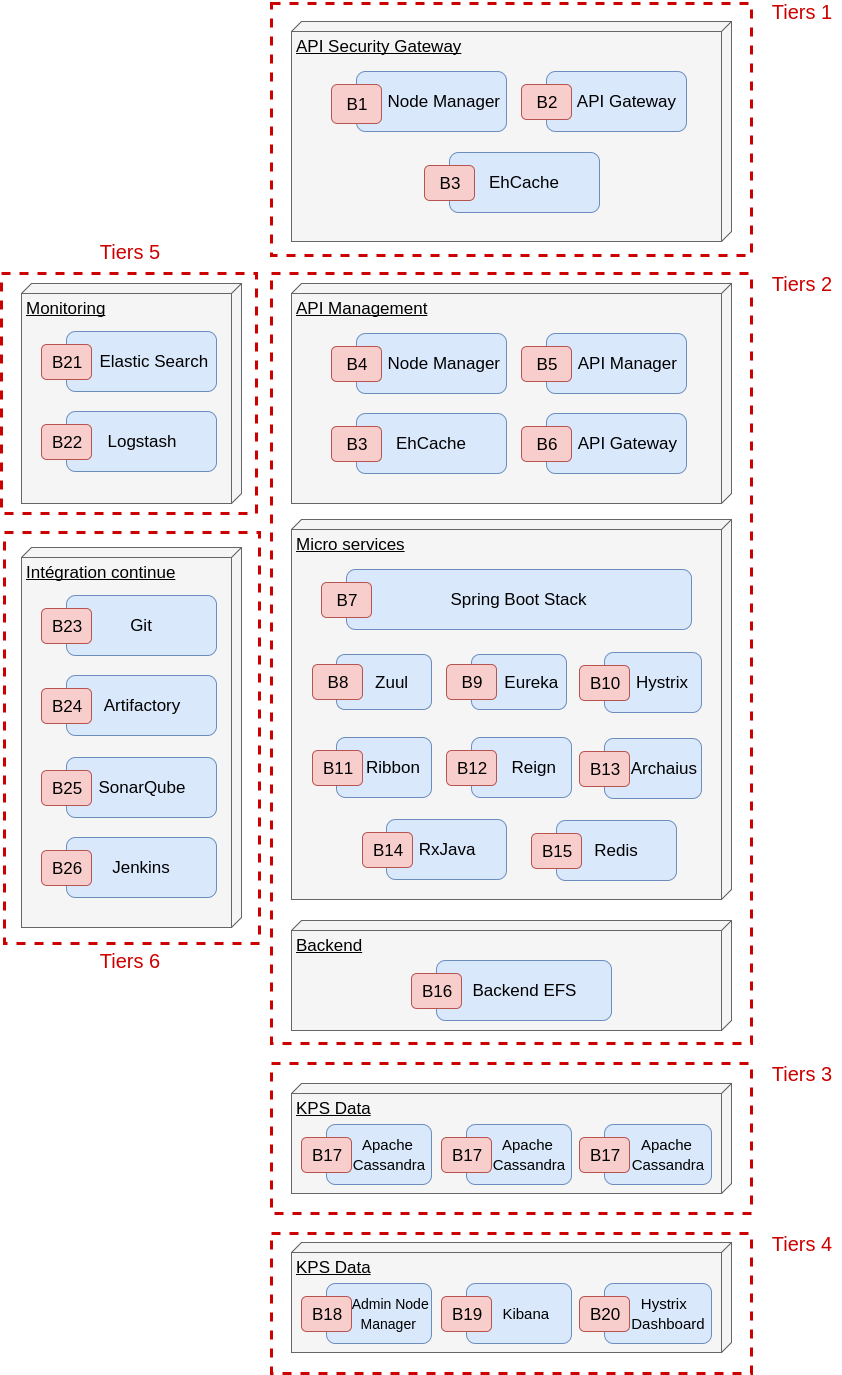
\includegraphics[scale=0.45]{images/travailNeuflizeOBC/architecture/architectureLogicielle.png}
	\centering
	\caption{Architecture logicielle - Neuflize OBC}
	\label{archiLog}
\end{figure}
	
	\chapter{Fonctionnalités clées - Neuflize OBC}
	\label{a2}
	\fancyhead[LE]{
	\begin{picture}(0,0) 
	\put(-30,-8){
\includegraphics[width=49mm]{images/neuflizeOBCLogo.png}}
	\end{picture}
}
\fancyhead[LO]{
	\begin{picture}(0,0) 
	\put(-8,-8){
\includegraphics[width=49mm]{images/neuflizeOBCLogo.png}}
	\end{picture}
}

\begin{figure}[H]
\raggedleft
	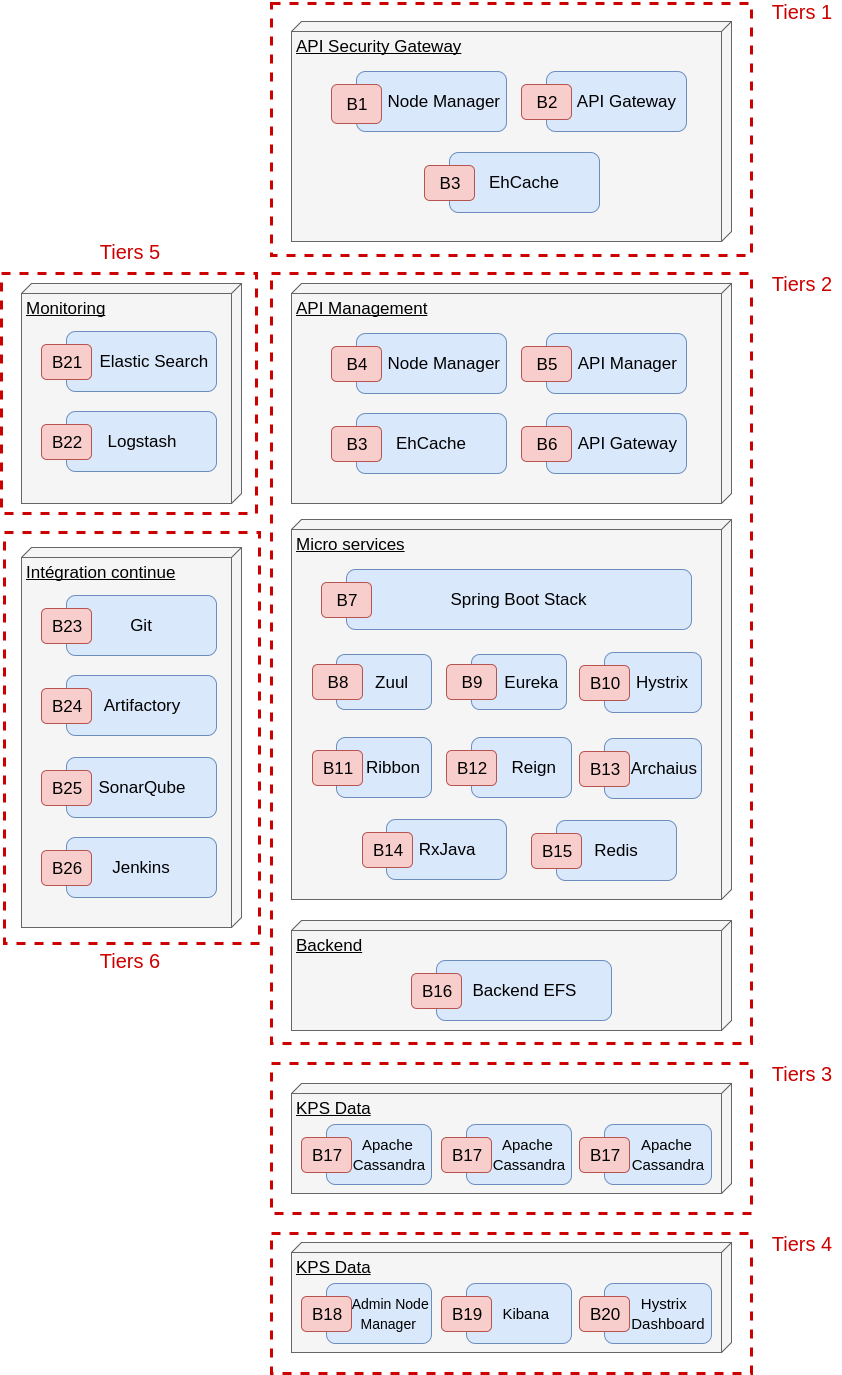
\includegraphics[scale=0.45]{images/travailNeuflizeOBC/architecture/architectureLogicielle.png}
	\centering
	\caption{Architecture logicielle - Neuflize OBC}
	\label{archiLog}
\end{figure}
	
	\chapter{Authentification - Neuflize OBC}
	\label{a3}
	A ke koukou chéma d'otantifikation !

\hl{TODO : voir avec Rudy (et Ali si besoin infos gateway)}
	
\end{appendices}
%-----------------------------------------------------------------------------------------------------------------
%-----------------------------------------------------------------------------------------------------------------
\newpage
\newpage
% Page blanche

\end{document}
